\documentclass{cernrep}
%% Language and font encodings
\usepackage[english]{babel}
\usepackage[utf8x]{inputenc}
\usepackage[T1]{fontenc}
\usepackage{pdflscape}

%% Sets page size and margins
\usepackage[a4paper,top=3cm,bottom=2cm,left=3cm,right=3cm,marginparwidth=1.75cm]{geometry}

%% Useful packages
\usepackage{amsmath}
\usepackage{graphicx}
\usepackage[colorinlistoftodos]{todonotes}
\usepackage[colorlinks=true, allcolors=blue]{hyperref}
\pagestyle{plain}
\newcommand{\Zp}{\ensuremath{Z^{\prime}}}
\newcommand{\ZpSSM}{\ensuremath{Z^{\prime}_{\mathrm{SSM}}}}
\newcommand{\Z}{\ensuremath{Z}}
\newcommand{\ttbar}{\ensuremath{t\bar{t}}}
\newcommand{\ptSub}[1]{\ensuremath{p_{\text{T} #1}}}
\newcommand{\ptSup}[1]{\ensuremath{p_{\text{T}}^{#1}}}
\newcommand{\pt}{\ensuremath{p_{\text{T}}}}
\newcommand{\ptEl}{\ensuremath{p_{\text{T}}^{e}}}
\newcommand{\ptMu}{\ensuremath{p_{\text{T}}^{\mu{}}}}
\newcommand{\ptZp}{\ensuremath{p_{\text{T}}^{\ensuremath{Z^{\prime}}}}}
\newcommand{\mZp}{\ensuremath{M_{\ensuremath{Z^{\prime}}}}}
\newcommand{\mll}{\ensuremath{M_{\ensuremath{ll}}}}

\def\ifb{\mbox{fb$^{-1}$}}%  Inverse femtobarns.
\def\afb{\mbox{ab$^{-1}$}}%  Inverse femtobarns.

\def\TeV{\ifmmode {\mathrm{\ Te\kern -0.1em V}}\else
                   \textrm{Te\kern -0.1em V}\fi}%
\def\GeV{\ifmmode {\mathrm{\ Ge\kern -0.1em V}}\else
                   \textrm{Ge\kern -0.1em V}\fi}%
\def\MeV{\ifmmode {\mathrm{\ Me\kern -0.1em V}}\else
                   \textrm{Me\kern -0.1em V}\fi}%
\def\keV{\ifmmode {\mathrm{\ ke\kern -0.1em V}}\else
                   \textrm{ke\kern -0.1em V}\fi}%
\def\eV{\ifmmode  {\mathrm{\ e\kern -0.1em V}}\else
                   \textrm{e\kern -0.1em V}\fi}%


%%%%%%%% for commenting in the text (editors add your alias here)%%%%%%%%%%
\newcommand{\HG}[1] {\textbf{\textcolor{red}{HG - #1}}}
\newcommand{\FM}[1] {\textbf{\textcolor{blue}{FM - #1}}}
\newcommand{\MS}[1] {\textbf{\textcolor{purple}{MS - #1}}}

\newcommand*{\Zptata}{\ensuremath{Z^{\prime}\rightarrow \tau\tau}}
\newcommand*{\Zpee}{\ensuremath{Z^{\prime}\rightarrow \text{e e}}}
\newcommand*{\Zpmumu}{\ensuremath{Z^{\prime}\rightarrow \mu\mu}}
\newcommand*{\Zpll}{\ensuremath{Z^{\prime}\rightarrow \ell\ell}}
\newcommand*{\Zptt}{\ensuremath{Z^{\prime}\rightarrow \ttbar}}
\newcommand*{\hht}{\ensuremath{H_{\ensuremath{T}}}}
\newcommand*{\met}{\ensuremath{E_{T}^{\rm{miss}}}}
\newcommand*{\intlumifcc}{\ensuremath{\mathcal{L}=30\text{ ab}^{-1}}}
\newcommand*{\intlumihelhc}{\ensuremath{\mathcal{L}=15\text{ ab}^{-1}}}
\newcommand*{\zptt}{\ensuremath{Z^{\prime} \rightarrow \ttbar}}
\newcommand*{\qjj}{\ensuremath{Q^{*} \rightarrow jj}}
\newcommand*{\rsg}{\ensuremath{G_{RS} \rightarrow WW}}
\newcommand*{\vj}{\ensuremath{\text{V + jets}}}
\newcommand*{\metvec}{\vec{\pt}^{\textrm{miss}}}

\begin{document}
\title{FCC Physics: Heavy resonances $\Zp$, RS graviton and $Q^{*}$ at $\sqrt{s} = 100 \TeV$}
\author{Clement Helsens${}^1$,\,
David Jamin${}^2$,\,
Michele Selvaggi${}^1$}
\institute{${}^1$ CERN, Geneva, Switzerland \newline
${}^2$ Academia Sinica, Taipei City, Taïwan}

%di-jet
%https://arxiv.org/pdf/1703.09127.pdf
%ATLAS INT NOTE ttbar res 
%https://cds.cern.ch/record/1640960/files/ATL-COM-PHYS-2014-003.pdf

\begin{abstract}
This paper explores the physics reach of the proton-proton Future Circular Collider (FCC-hh)
for searches of new particles decaying to two high energetic leptons($l^{+}l^{-}$ or $\tau^{+}\tau^{-}$), jets (non-tops), tops and W/Z boson. We discuss the expected exclusion limits and discovery potential for benchmark models 
predicting new massive particles that result in resonant structures in
the invariant mass spectrum. The study is based on the Madgraph5 and Pythia8 Monte Carlo generators using large event statistics for the FCC running conditions. 
Its unprecedented  
This document presents a detailed study on the discovery potential of heavy gauge resonance $\Zp$ and center of mass energy $\sqrt[]{s} =100$~TeV makes it the ultimate machine for such new particles, and are also extremely relevant to discuss the main limitations of the detector to tag high energetic top-quarks or W/Z bosons.
\end{abstract}
\keywords{CERN report; FCC.}
\maketitle
\tableofcontents

\section{Introduction}
The design of a 100 TeV proton-proton collider leads to many challenges for detector design. Detailed optimizations of the detector is needed in order to achieve the required physics goals. The capabilities of such a detector should include the capabilities of measuring multi-TeV leptons, top-quarks and bosons.

%%%%%%%%%%%%%%%%%%%%%%%%%%%%%%%%%%%%%%%%%%%%%%%%%%%%%
%%%%%%%%%%%%%%%%%%%%%%%%%%%%%%%%%%%%%%%%%%%%%%%%%%%%%
\section{FCC work flow}
\label{sec:fccworkflow}

%%%%%%%%%%%%%%%%%%%%%%%%%%%%%%%%%%%%%%%%%%%%%%%%%%%%%
\subsection{Monte-Carlo production}
\label{subsec:mcprod}

All the signal Monte-Carlo events have been produced directly with Pythia 

%%%%%%%%%%%%%%%%%%%%%%%%%%%%%%%%%%%%%%%%%%%%%%%%%%%%%
\subsubsection{Fit model}
Despite the fact that very large amount of Monte-Carlo statistic has been simulated in bins of $\hht$, there are still large statistical fluctuations from high weight events.
In order to reduce this effect, a function is used to fit the background distribution,
\begin{equation}
f(z)=p_1(1-z)^{p_2}z^{p_3}z^{p_{4}logz}
\end{equation}
where $z=m_{jj}/\sqrt{s}$. This fit is used in order to have a smooth shape for the backgrounds, while the normalisation is taken prior to the fit (see figure~\ref{fig:hadronicresonances_nofit}).

\begin{figure}[!htb]\centering
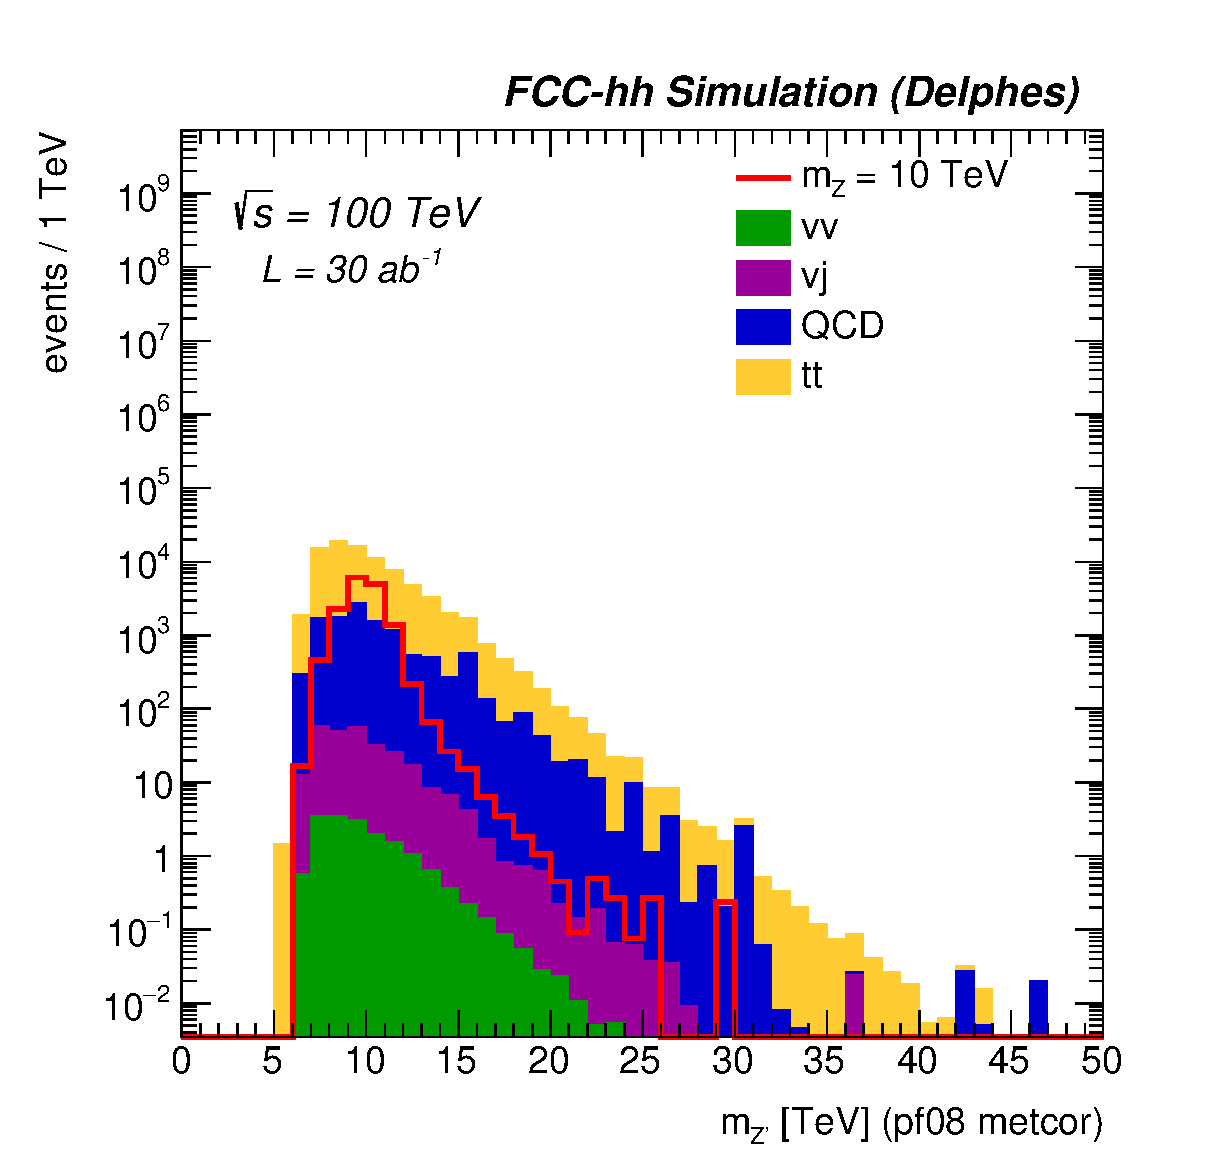
\includegraphics[width=0.45\columnwidth]{Fig/Zptt/Mj1j2_pf08_MetCorr_sel8_nostack_log.eps}
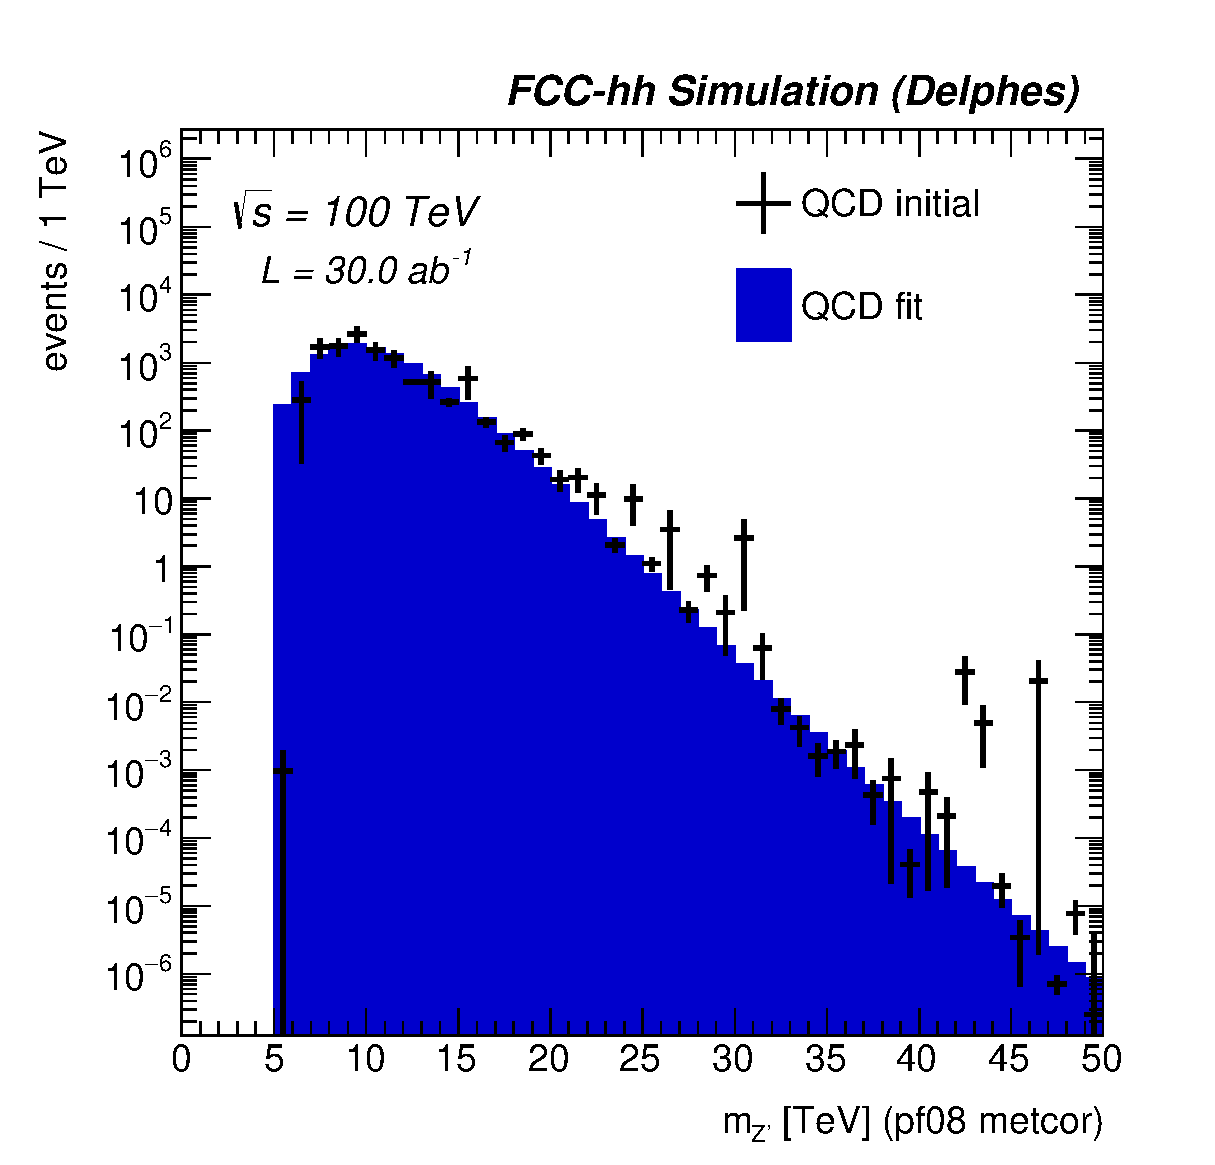
\includegraphics[width=0.45\columnwidth]{Fig/Zptt/Zptt_QCD_sel8_Mj1j2_pf08_MetCorr_fit.eps}
\caption{Invariant mass prior to fit.}
\label{fig:hadronicresonances_nofit}
\end{figure}

%%%%%%%%%%%%%%%%%%%%%%%%%%%%%%%%%%%%%%%%%%%%%%%%%%%%%%%%%%%%%%%%%%%%%%%%%%%%%%%%%%%%%%%%%%%%
\subsection{Detector parameterizations}
\label{subsec:detparam}

The FCC study group is using the Delphes software package to emulate the response a detector. 
For the FCC one the baseline parameters are:
We also consider two variations around it as well as the CMS configuration.


%%%%%%%%%%%%%%%%%%%%%%%%%%%%%%%%%%%%%%%%%%%%%%%%%%%%%
\subsection{Multi-Variate based selection}
\label{subsec:mvatagger}

% from physics paper
An important ingredient of the \zptt\ and \rsg\ searches is the identification of heavy boosted top quarks and $W$ bosons. Two jet taggers using Boosted Decision Trees (BDTs) were developed to discriminate $W$ and top jets against the $\pt$ di-jet background.

Top and $W$ taggers were optimised using jets with a transverse boost of $\pt=$10 TeV. At these extreme energies, $W$ and top jets have a characteristic angular size $R=0.01-0.02$, i.e smaller than the typical electromagnetic and hadronic calorimeter cells. Following the approach described in~\cite{Larkoski:2015yqa}, we exploit the superior track angular resolution and reconstruct jets from tracks only (track jets) using the anti-$k_T$ algorithm with a parameter R=0.2. The missing neutral energy is corrected for by rescaling the track 4-momenta by the factor $\ptSup{trk}/\ptSup{PF}$, where $\ptSup{trk}$ is the track Jet \pt\ and $\ptSup{PF}$ is the Particle-Flow Jet \pT. In what follows, we will simply refer to ``track jets'' as the jet collection that includes the aforementioned rescaling.

The boosted top tagger is built from jet substructure observables: the soft-dropped jet mass~\cite{Larkoski:2014wba} and N-subjettiness~\cite{Thaler:2010tr} variables $\tau_{1,2,3}$ and their ratios $\tau_{2}/\tau_{1}$ and $\tau_{3}/\tau_{2}$. The $W$-jet versus QCD-jet tagger also uses an ``isolation-like'' variable that exploits the absence of high \pt\ final state-radiation (FSR) in the vicinity of the $W$ decay products. We call these variables $E_{F}(n,\alpha)$ and define them as:

\begin{equation}
E_{F}(n,\alpha) =  \frac{\sum \limits_{\frac{n-1}{5}\alpha < \Delta R(k,jet)< \frac{n}{5}\alpha} \ptSup{(k)}}{\sum \limits_{\Delta R(k,jet)< \alpha} \ptSup{(k)}}
\end{equation}

We use $\alpha=0.05$. We construct 5 variables $E_{F}(n,\alpha)$ with $n=1..5$ and provide them as input to the BDT. The $E_{F}(1,0.05)$ observable is shown in Figure~\ref{figure:hadronicresonances:BDTeff} (left).
The final performance of the $W$ and top tagger is shown in Figure~\ref{figure:hadronicresonances:BDTeff} (right). The $W$ tagging performance has significantly better performance due to the use of the energy-flow variables. We choose our working points with a top and $W$ tagging efficiencies of $\epsilon_S^{\text{top}}=60\%$ and $\epsilon_S^{\text{W}}=90\%$ corresponding respectively to a background efficiency of $\epsilon_B^{\text{top}}=\epsilon_B^{\text{W}}=10\%$.

% plots are shown later
%\begin{Figure}
%  \centering
%  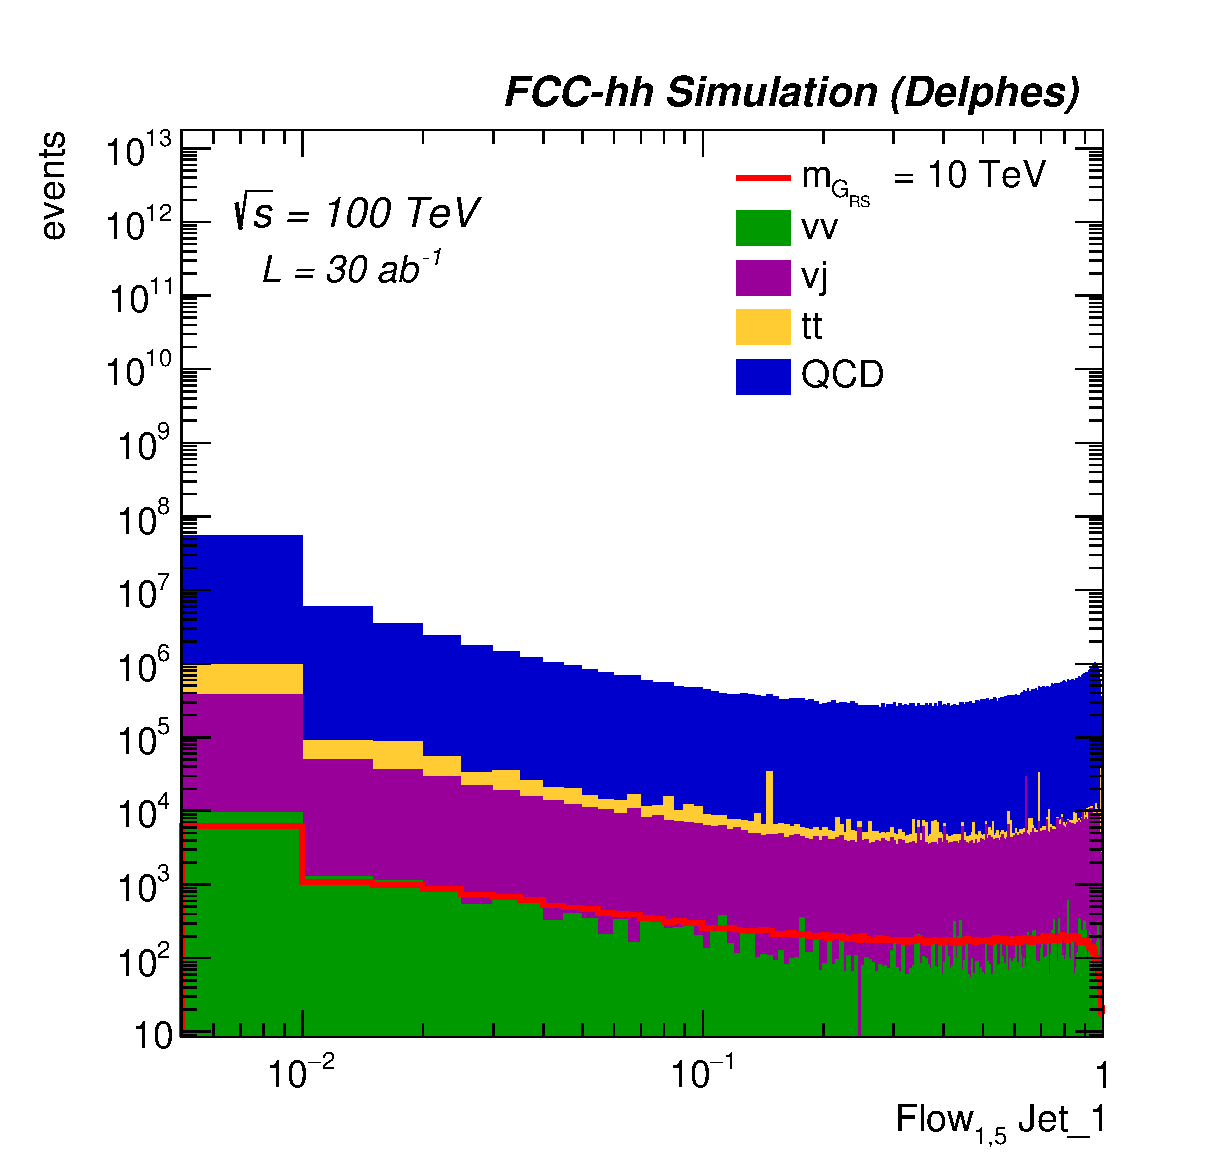
\includegraphics[width=0.37\columnwidth]{\main/img/hadronicresonances/Jet1_Flow15_sel0_nostack_logx.eps}
%  \includegraphics[width=0.45\columnwidth]{\main/img/hadronicresonances/effQCD_vs_effWhadBlue_thadRed_log.eps}
%  \caption{Left: Energy-flow ($E_{F}(1,0.05)$) observable for W and QCD jets. Right: Di-jet rejection versus signal efficiency for the two taggers, W in blue and top in red.%\MS{need editing - REDO left EFlow in logX - Right: need legend and stars}
%  }
%  \label{figure:hadronicresonances:BDTeff}
%\end{Figure}

% raw infos
- design 2 taggers to perform Whad and thad separation with QCD,
- made pythia independent samples from analysis, QCD has been produced to avoid useless events and to perform that the filtering has been chosen to ensure to have similar signal leading jet $\pT$ (pTHatMin = 2500, bias2Selection = on, bias2SelectionPow = 6.)
- the statistics obtained for Whad, thad and QCD are respectively 1M, 1M and 920k events with 2 jets, each jet will be an entry for the BDT training,
%- the BDT parameters for training are : !H:!V:NTrees=600:MaxDepth=4:BoostType=AdaBoost:AdaBoostBeta=0.15:SeparationType=GiniIndex:nCuts=100:PruneMethod=NoPruning
- a training selection is applied to remove uselees events with isolated leptons and jets for which jet $\tau$ ratio variables failed (i.e has a negative value)
- the training statistics obtained for Whad, thad and QCD are respectively 1117500, 1432192 and 1578098 jets, half of the stat is used for training and the other half for testing
- the variables are defined to be the same as the ones used to perform cut-based associated analysis ($\Zp \rightarrow \ttbar$ in section~\ref{subsec:Zptt} and $G \rightarrow WW$ in section~\ref{subsec:RSGww} ) and the idea is to fully exploit these informations thanks to the BDT, variable list and ranking in table~\ref{tab:TMVA_summary}
- the BDT performances in plots, 
- removing fully correlated variables have tried and doesn't change anything to performances shown
- the BDT response has been shown (\ref{fig:BDT_signal_shape_comparison}) for different signal masses generation to see how much analysis can be mass dependent. From the cuts defined in the analysis level at 0.15, the BDT shape reponse difference is not changing so much the proportion of signal kept and it removes 90\% and 95\% of QCD for thad and Whad taggers respectively

\begin{table}[!htb]\centering
\begin{tabular}{|c|c|c|}
\hline
\hline			
 & Whad/QCD & thad/QCD \\
\hline                        
\hline                        
Sample signal     & p8\_pp\_RSGraviton\_20TeV\_ww & p8\_pp\_Zprime\_20TeV\_ttbar \\
Sample background & \multicolumn{2}{c|}{p8\_pp\_jj\_lo} \\
\hline      
Gen stat. signal (events)     & 1M & 1M \\
Gen stat. background (events) & \multicolumn{2}{c|}{920k} \\
\hline
train sel. &  \multicolumn{2}{c|}{no isolated leptons} \\
           &  \multicolumn{2}{c|}{Jet\_trk02 $\tau_{21}>0$, $\tau_{31}>0$, $\tau_{32}>0$} \\
\hline
Train stat. signal (jets)     & 1117500 & 1432192  \\
Train stat. background (jets) & \multicolumn{2}{c|}{1578098} \\
\hline
BDT params  &  \multicolumn{2}{c|}{NTrees=600, MaxDepth=4, AdaBoost, AdaBoostBeta=0.15,} \\
            &  \multicolumn{2}{c|}{SeparationType=GiniIndex, nCuts=100, PruneMethod=NoPruning} \\
\hline
ranked variables & Jet\_trk02\_tau3 (0.12)        & Jet\_trk02\_tau1 (0.21) \\
                 & Jet\_trk02\_SD\_Corr\_m (0.11) & Jet\_trk02\_SD\_Corr\_m (0.17) \\
                 & Jet\_trk02\_tau31 (0.10)       & Jet\_trk02\_tau31 (0.11) \\
                 & Jet\_Flow55 (0.09)             & Jet\_trk02\_tau2 (0.10) \\
                 & Jet\_Flow45 (0.09)             & Jet\_trk02\_tau3 (0.09) \\
                 & Jet\_Flow15 (0.08)             & Jet\_trk08\_SD\_Corr\_m (0.09) \\
                 & Jet\_Flow25 (0.07)             & Jet\_trk04\_SD\_Corr\_m (0.09) \\
                 & Jet\_Flow35 (0.06)             & Jet\_trk02\_tau32 (0.08) \\
                 & Jet\_trk02\_tau21 (0.06)       & Jet\_trk02\_tau21 (0.06) \\
                 & Jet\_trk08\_SD\_Corr\_m (0.06) &  \\
                 & Jet\_trk04\_SD\_Corr\_m (0.06) &  \\
                 & Jet\_trk02\_tau1 (0.05)        &  \\
                 & Jet\_trk02\_tau2 (0.04)        &  \\
                 & Jet\_trk02\_tau32 (0.02)       &  \\
\hline
\hline
\end{tabular}
\caption{Summary of BDT informations used to train Whad/thad VS QCD.}
\label{tab:TMVA_summary}
\end{table}

\begin{figure}[!htb]\centering
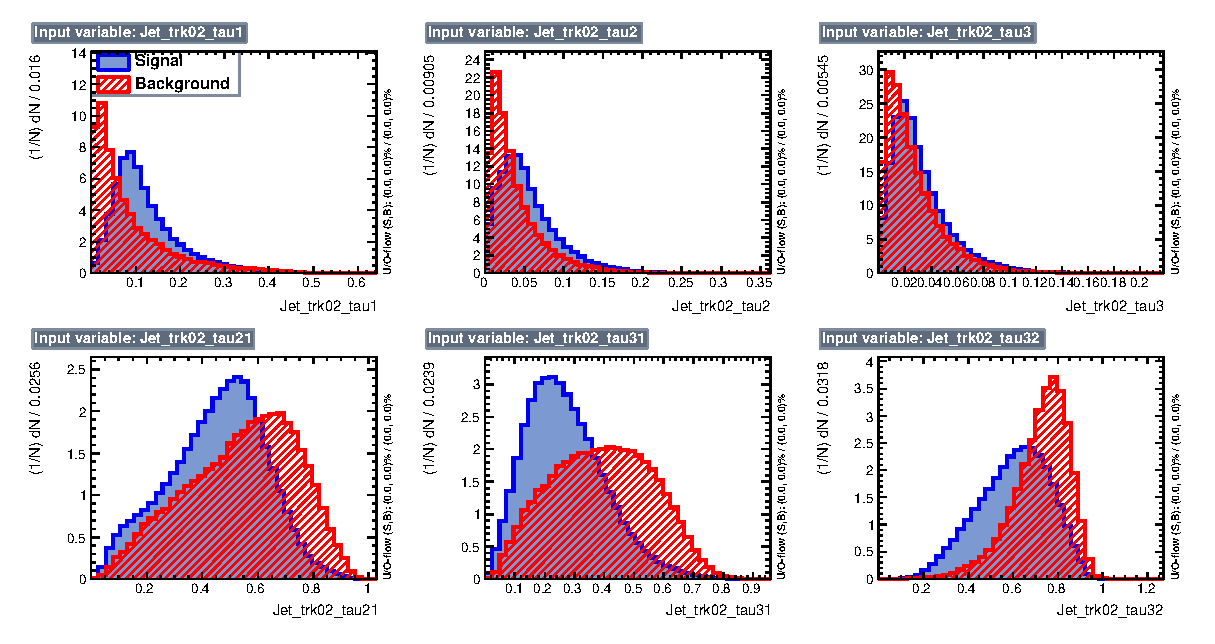
\includegraphics[width=0.495\textwidth]{Fig/TMVA/thad_vs_QCD/variables_id_c1.eps}
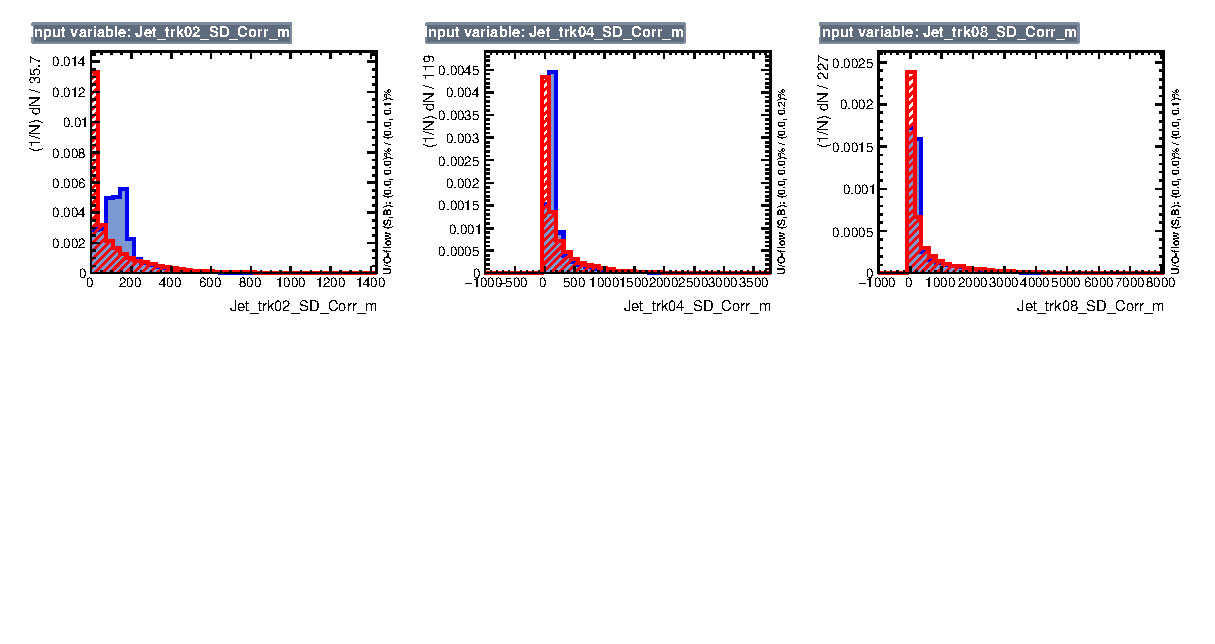
\includegraphics[width=0.495\textwidth]{Fig/TMVA/thad_vs_QCD/variables_id_c2.eps}
\caption{Input variables for top Vs QCD tagger.}
\label{fig:TMVA_inputs_t}
\end{figure}

\begin{figure}[!htb]\centering
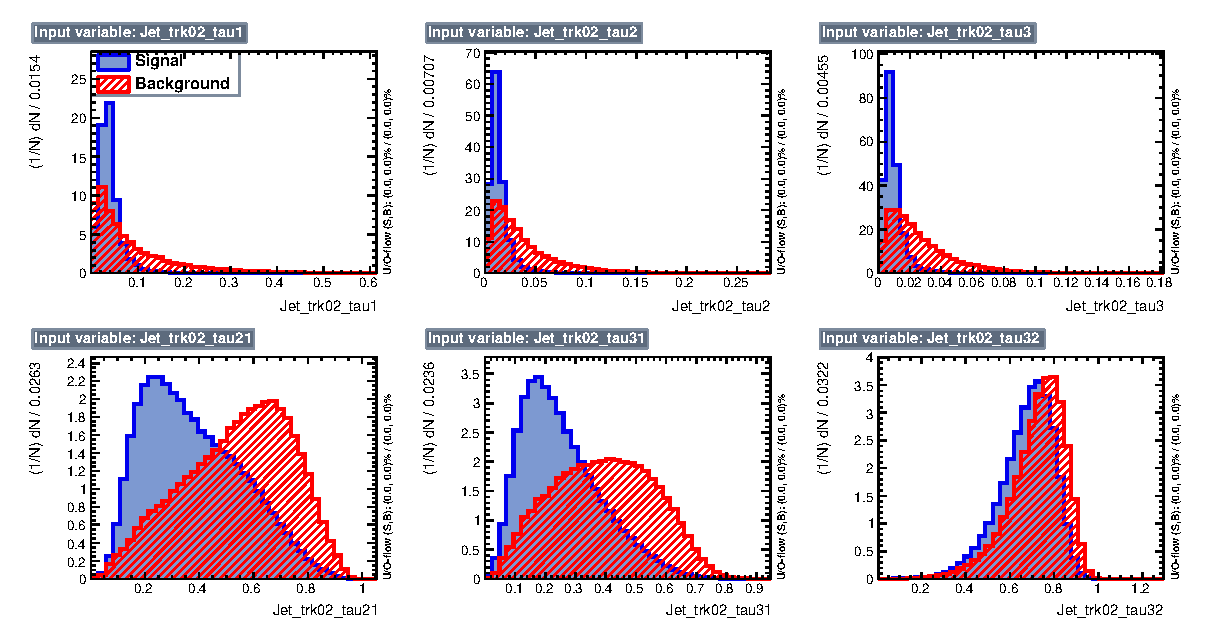
\includegraphics[width=0.495\textwidth]{Fig/TMVA/Whad_vs_QCD/variables_id_c1.eps}
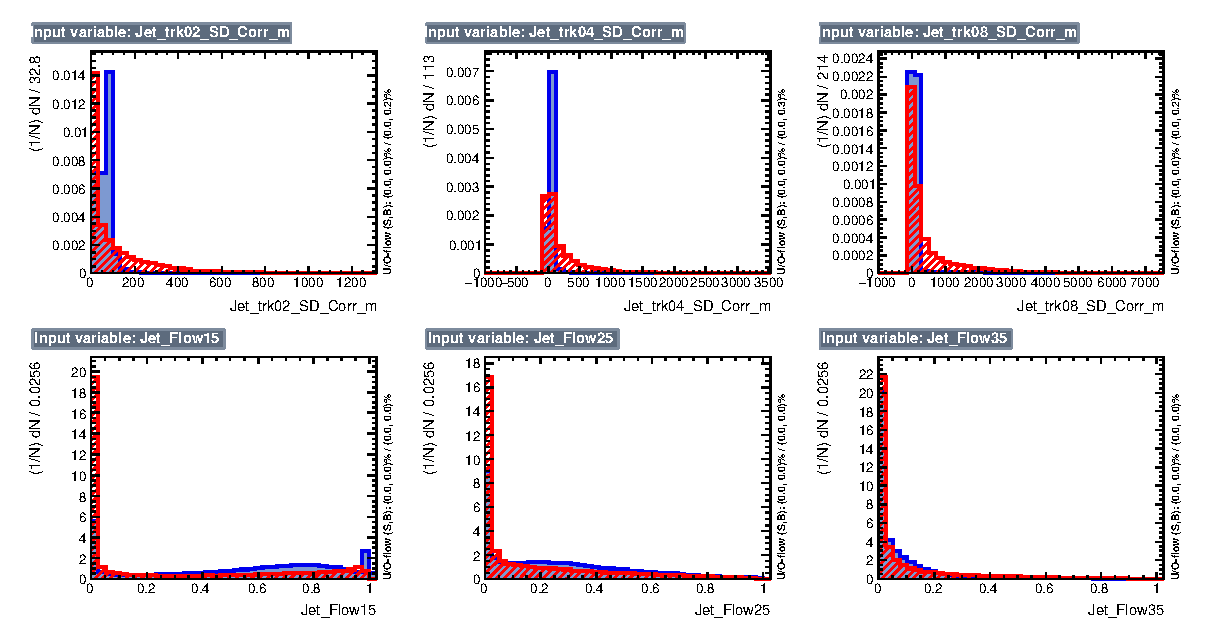
\includegraphics[width=0.495\textwidth]{Fig/TMVA/Whad_vs_QCD/variables_id_c2.eps}
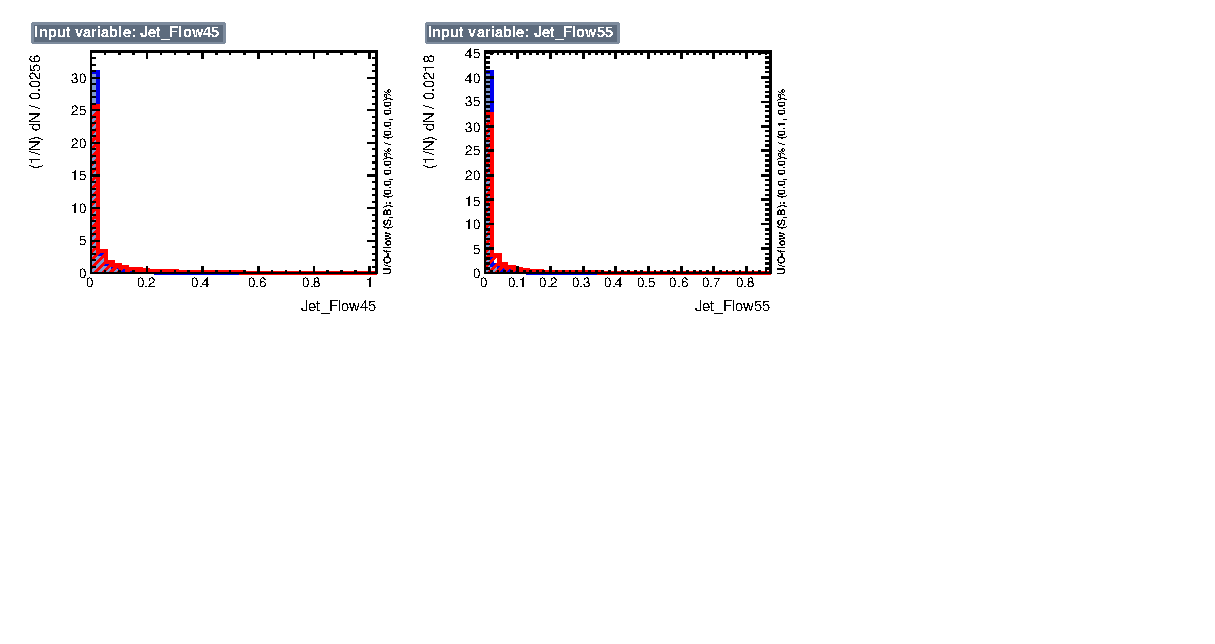
\includegraphics[width=0.495\textwidth]{Fig/TMVA/Whad_vs_QCD/variables_id_c3.eps}
\caption{Input variables for W Vs QCD tagger.}
\label{fig:TMVA_inputs_t}
\end{figure}

\begin{figure}[!htb]\centering
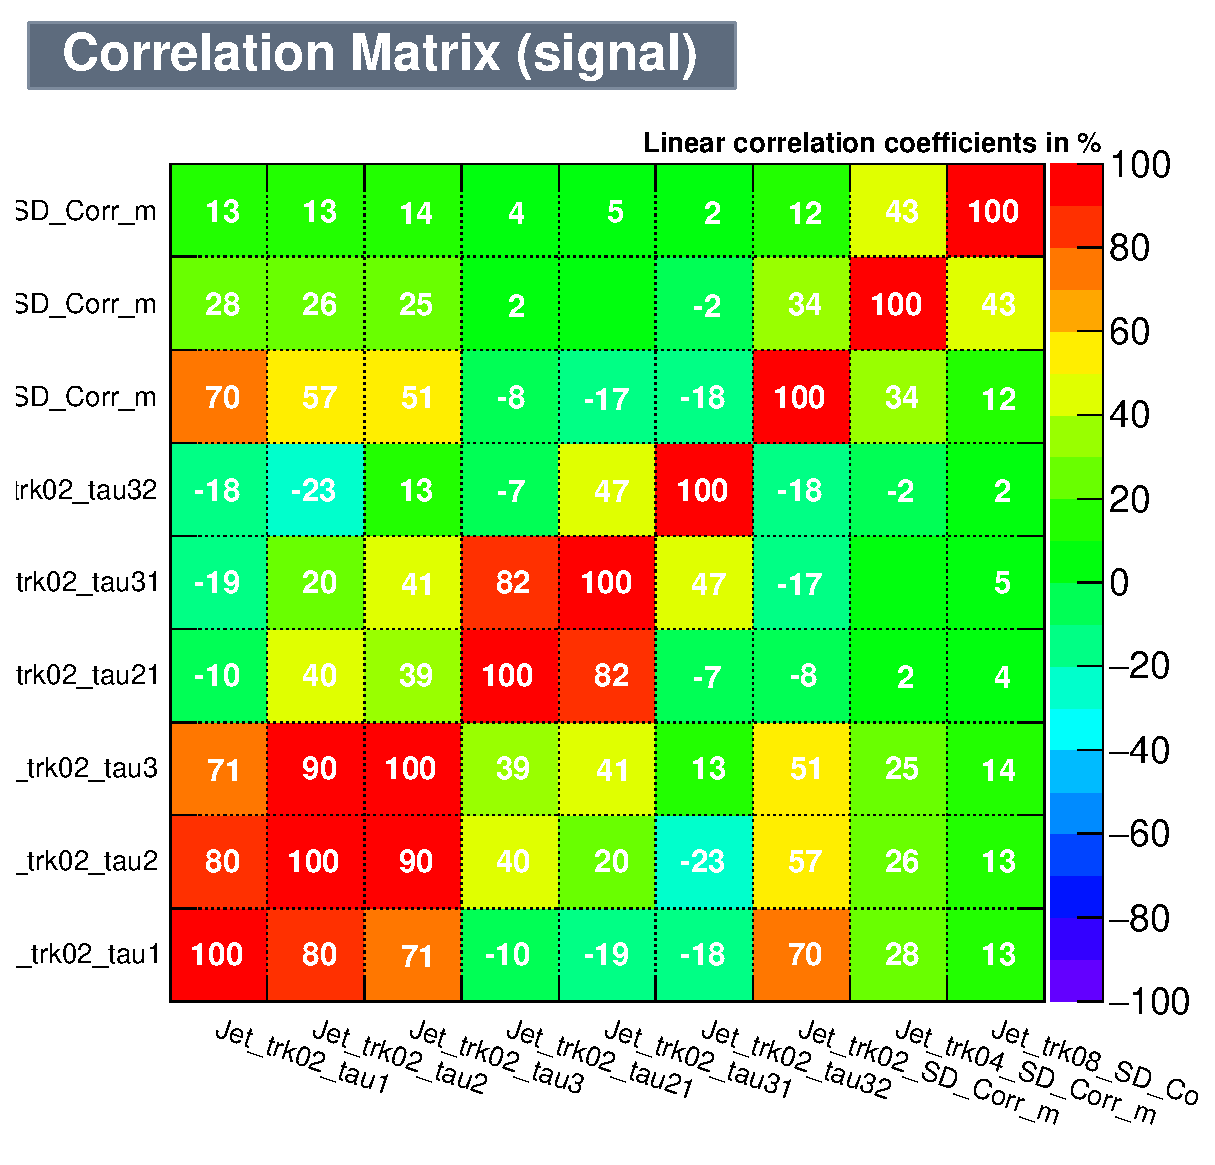
\includegraphics[width=0.495\textwidth]{Fig/TMVA/thad_vs_QCD/CorrelationMatrixS.eps}
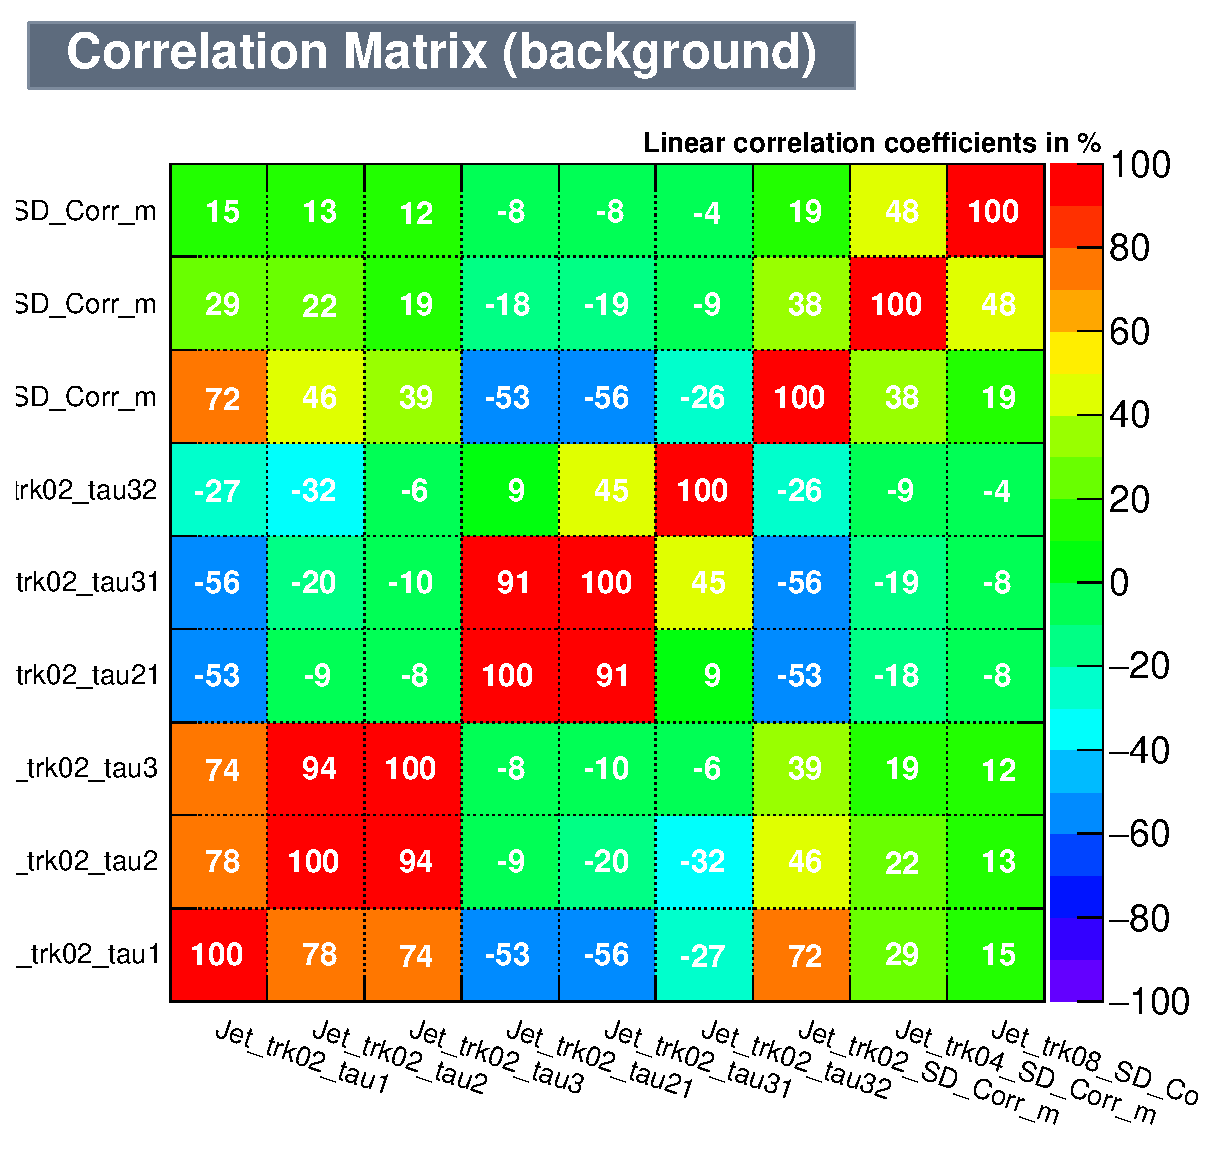
\includegraphics[width=0.495\textwidth]{Fig/TMVA/thad_vs_QCD/CorrelationMatrixB.eps}
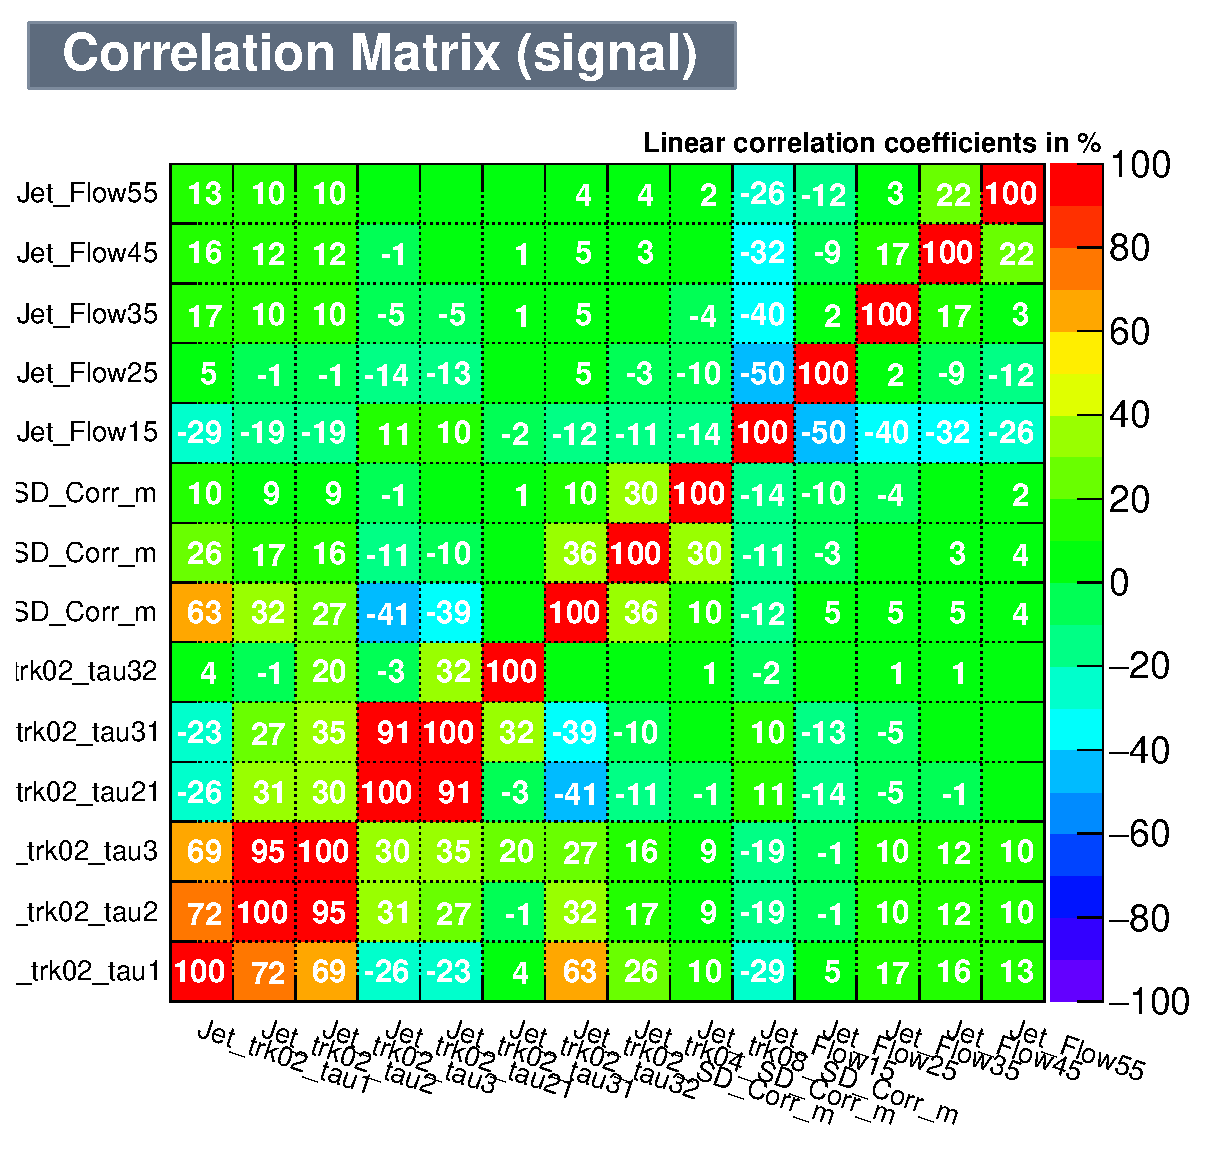
\includegraphics[width=0.495\textwidth]{Fig/TMVA/Whad_vs_QCD/CorrelationMatrixS.eps}
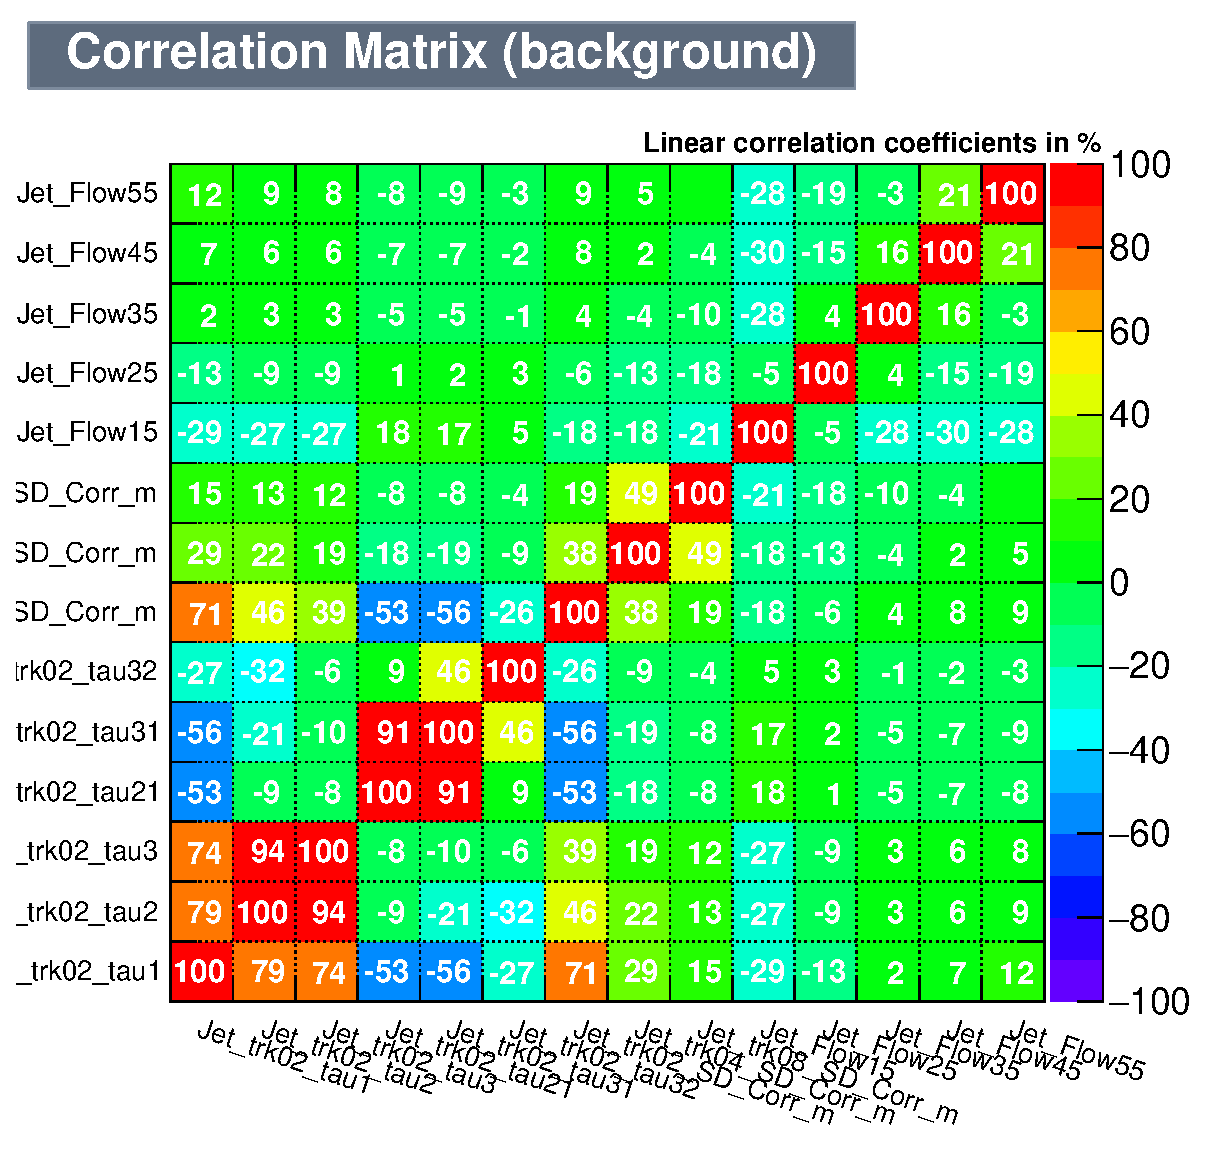
\includegraphics[width=0.495\textwidth]{Fig/TMVA/Whad_vs_QCD/CorrelationMatrixB.eps}
\caption{Correlation matrices for Signal (left) and Background (right) for top Vs QCD tagger (top) and W Vs QCD tagger (bottom).}
\label{fig:TMVA_corr_matrix}
\end{figure}

\begin{figure}[!htb]\centering
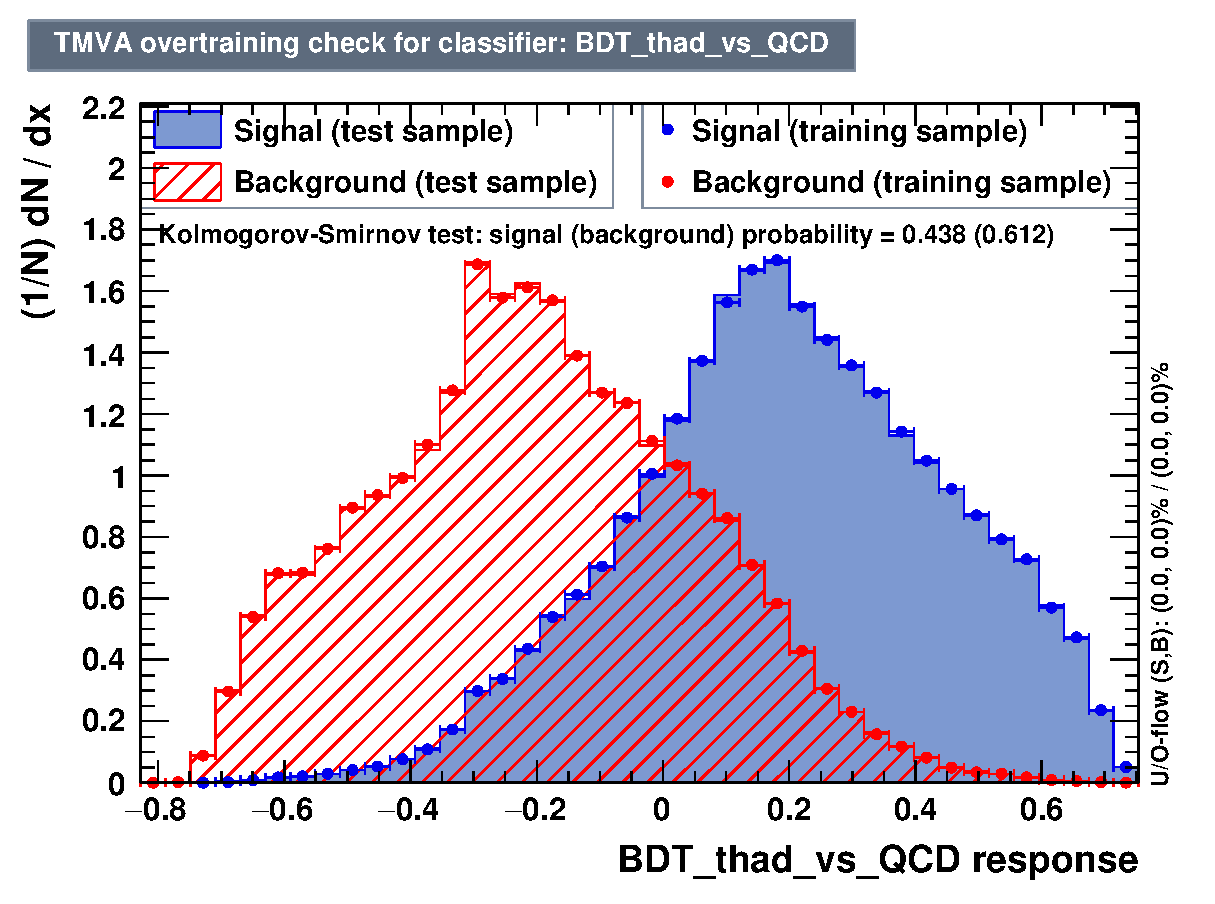
\includegraphics[width=0.495\textwidth]{Fig/TMVA/thad_vs_QCD/overtrain_BDT_thad_vs_QCD.eps}
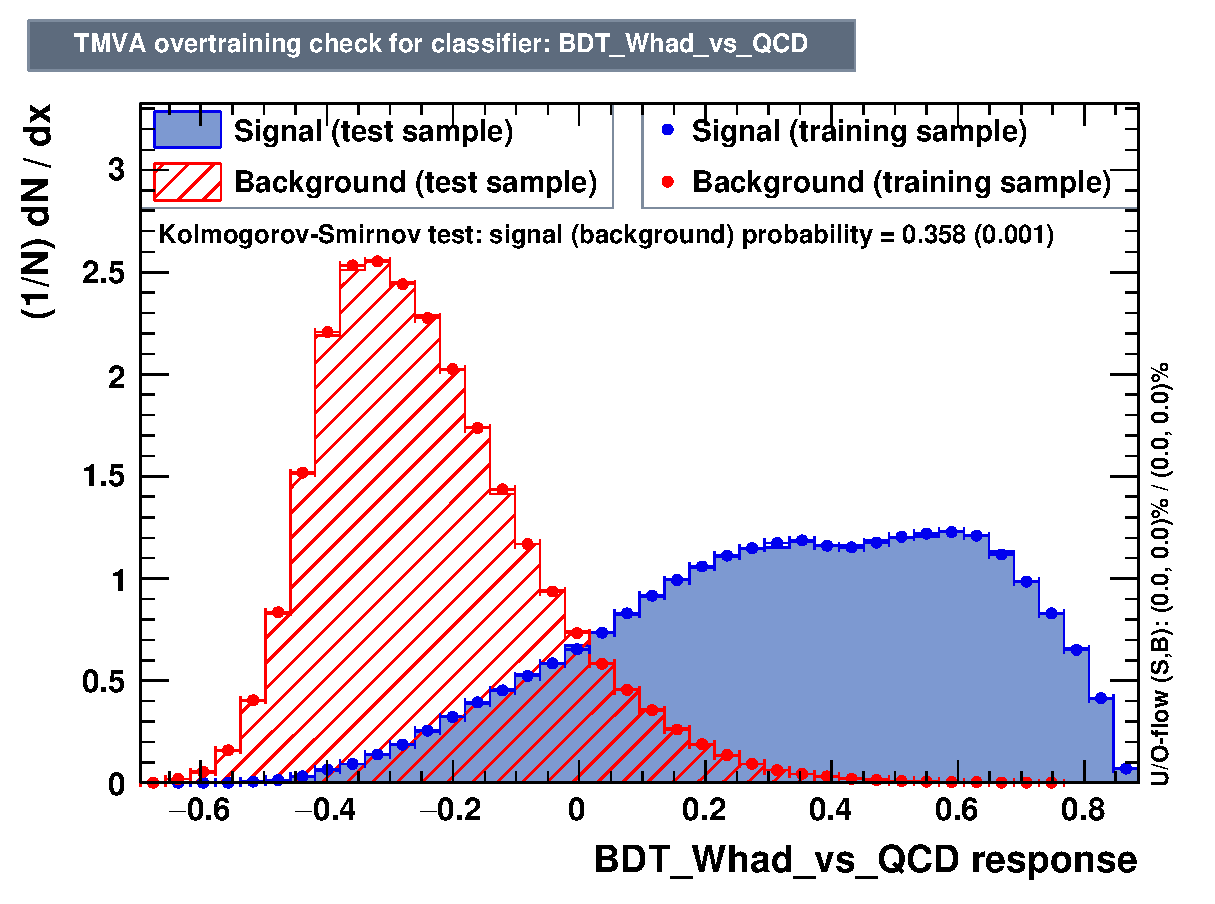
\includegraphics[width=0.495\textwidth]{Fig/TMVA/Whad_vs_QCD/overtrain_BDT_Whad_vs_QCD.eps}
\caption{BDT scores for Signal (red) and Background (blue) for top Vs QCD tagger (left) and W Vs QCD tagger (right).}
\label{fig:TMVA_BDTscore}
\end{figure}

\begin{figure}[!htb]\centering
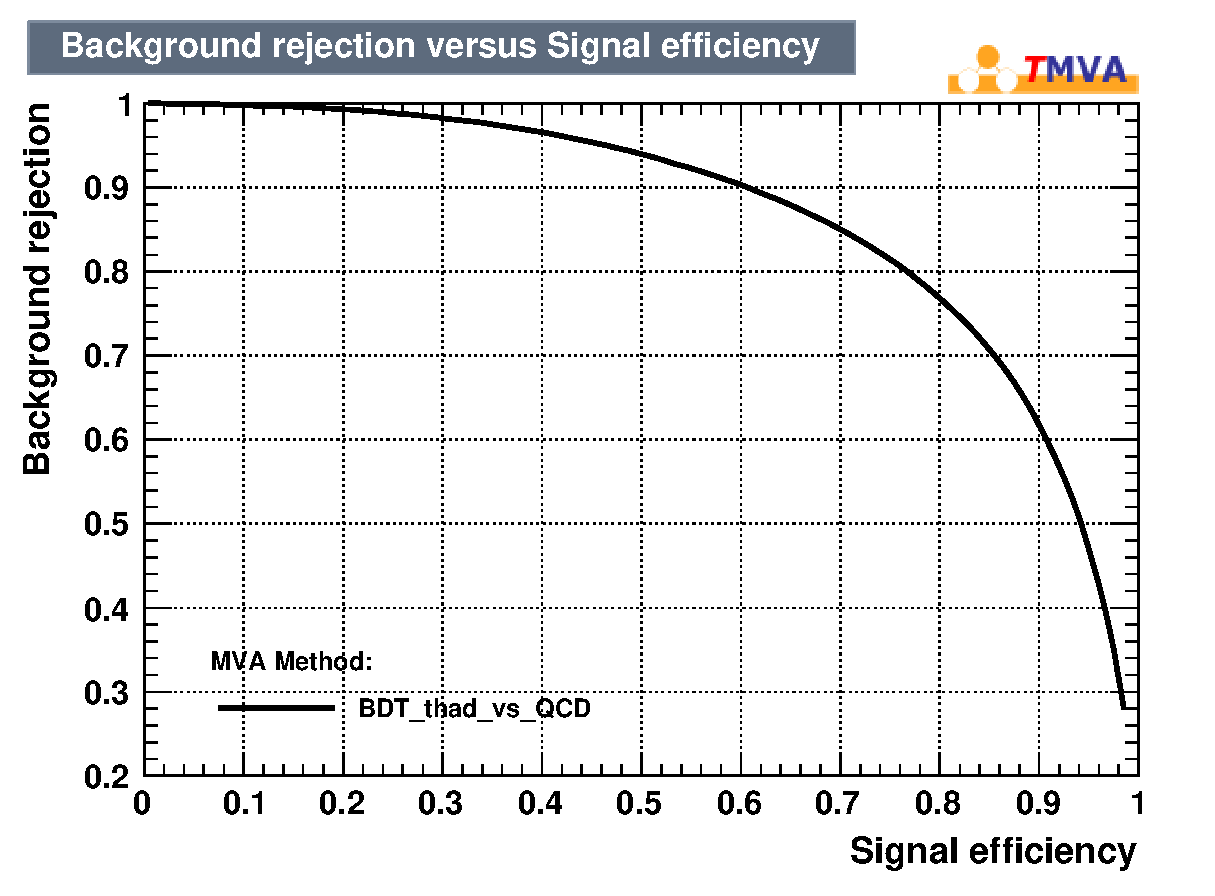
\includegraphics[width=0.495\textwidth]{Fig/TMVA/thad_vs_QCD/rejBvsS.eps}
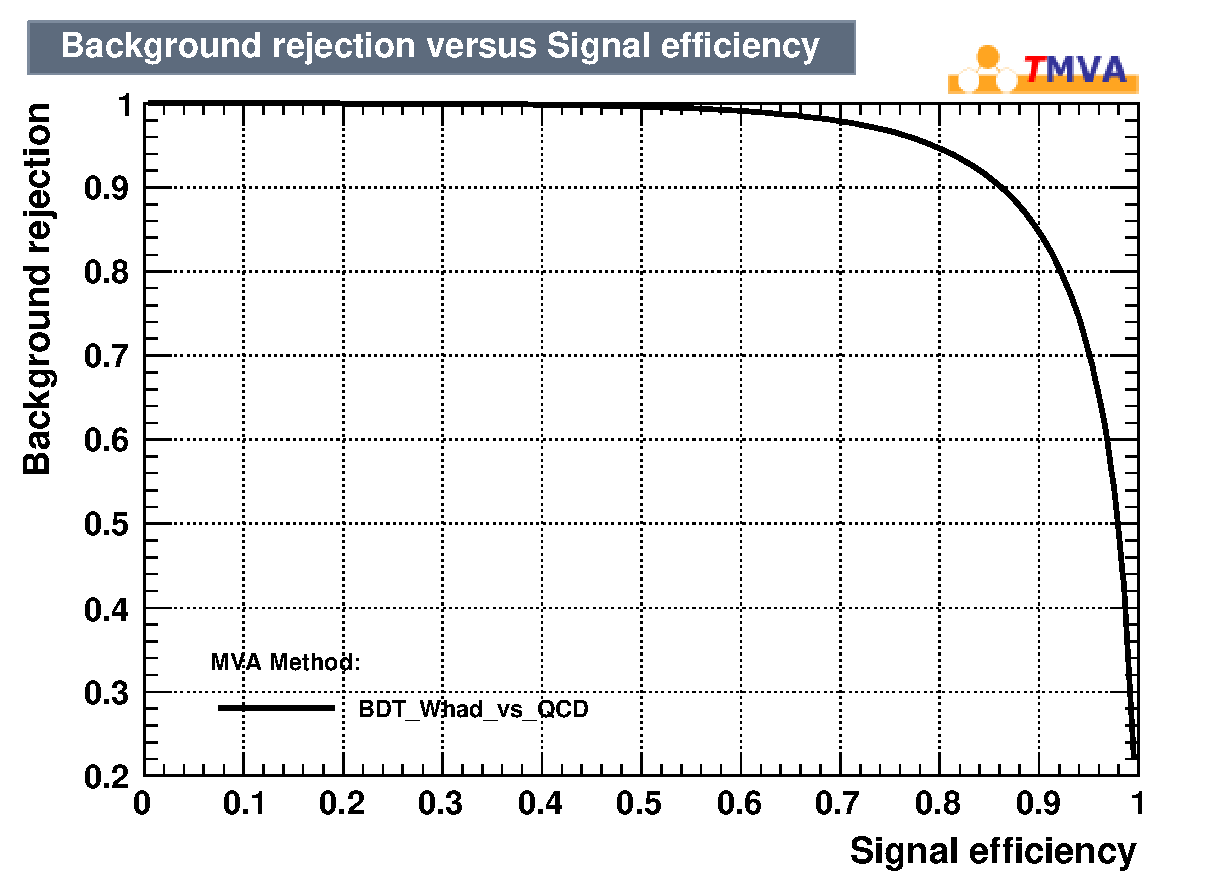
\includegraphics[width=0.495\textwidth]{Fig/TMVA/Whad_vs_QCD/rejBvsS.eps}
\includegraphics[width=0.495\textwidth]{Fig/TMVA/effQCD_vs_effWhadBlue_thadRed_log.eps}
\caption{Top ROC curves show background rejection Vs Signal efficiency for top Vs QCD tagger (left) and W Vs QCD tagger (right). Bottom ROC curves show background efficiency Vs signal efficiency overlay for top Vs QCD tagger (red) and W Vs QCD tagger (blue).}
\label{fig:TMVA_ROC}
\end{figure}

\begin{figure}[!htb]\centering
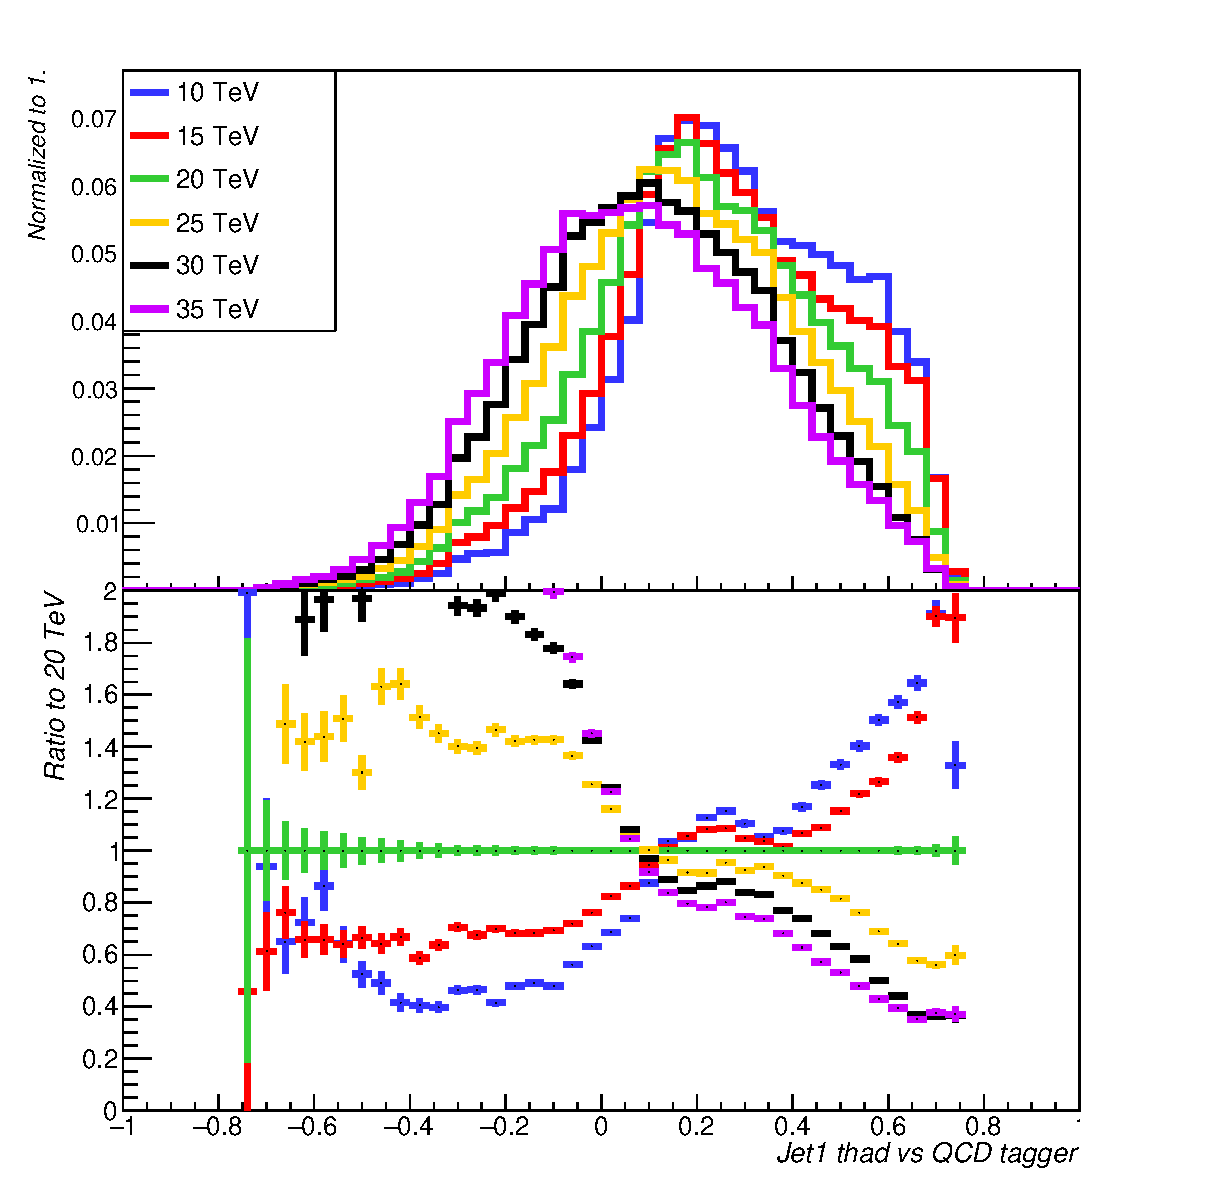
\includegraphics[width=0.495\textwidth]{Fig/TMVA/Jet1_thad_vs_QCD_tagger.eps}
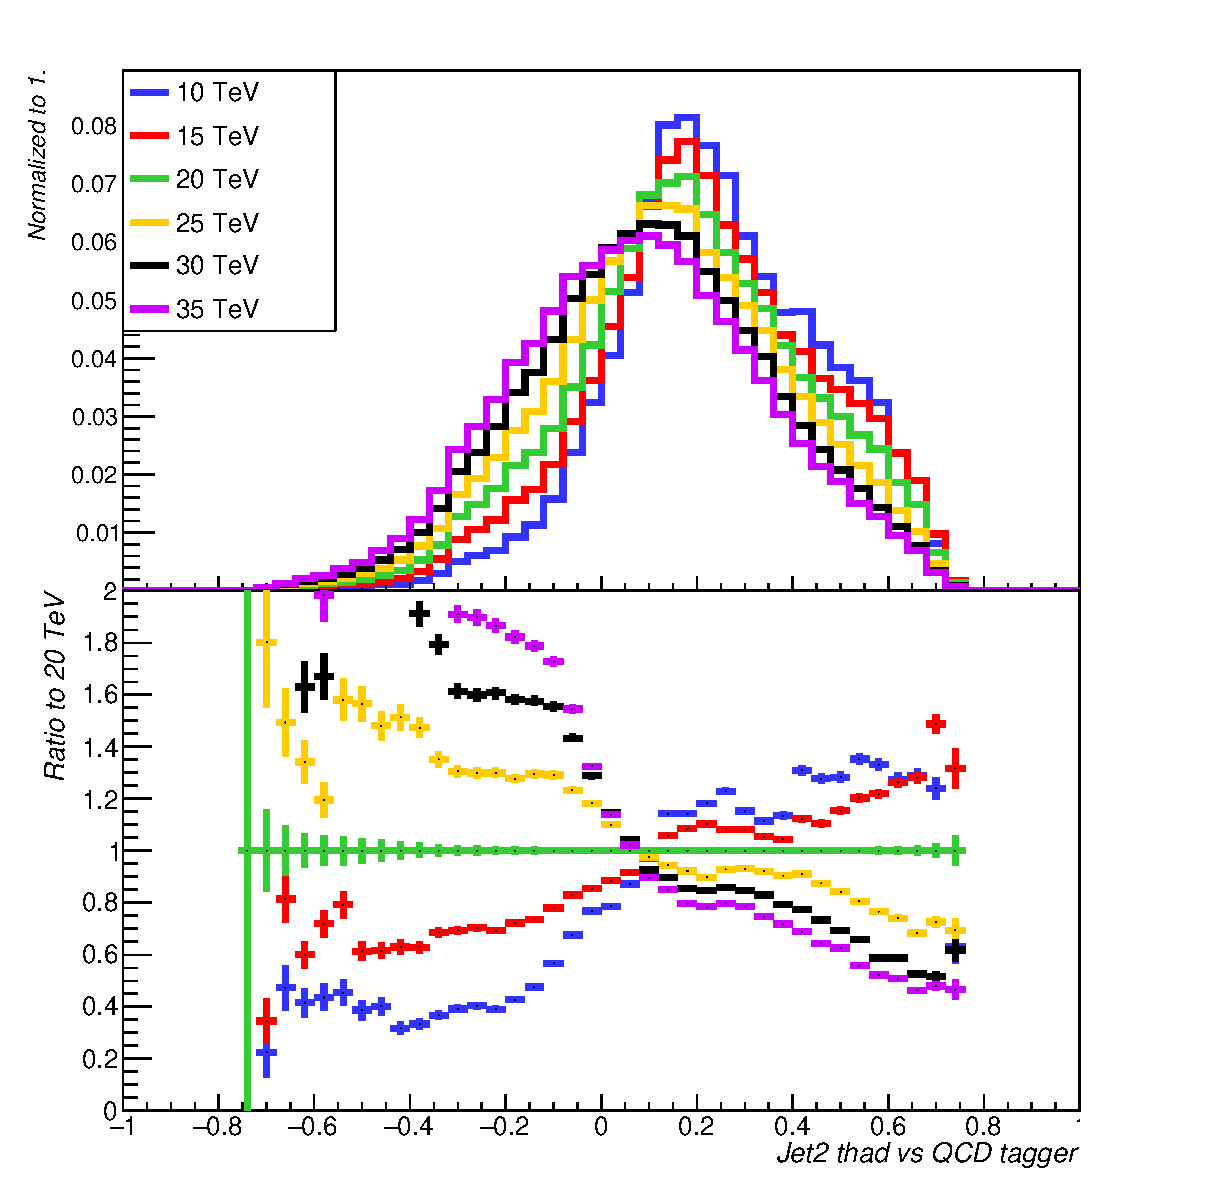
\includegraphics[width=0.495\textwidth]{Fig/TMVA/Jet2_thad_vs_QCD_tagger.eps}
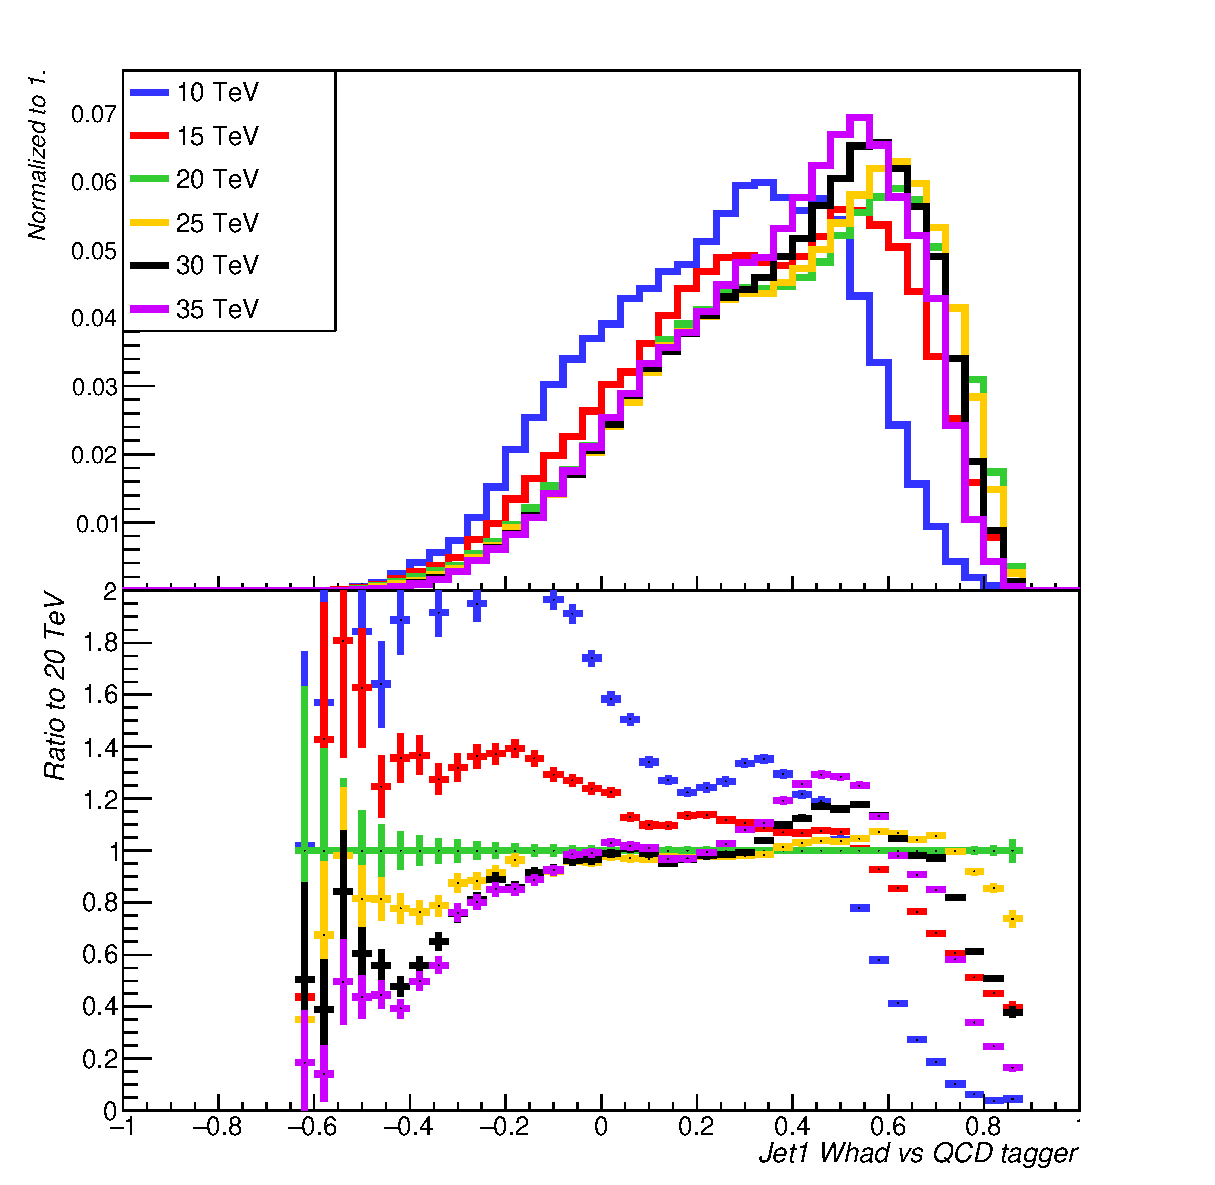
\includegraphics[width=0.495\textwidth]{Fig/TMVA/Jet1_Whad_vs_QCD_tagger.eps}
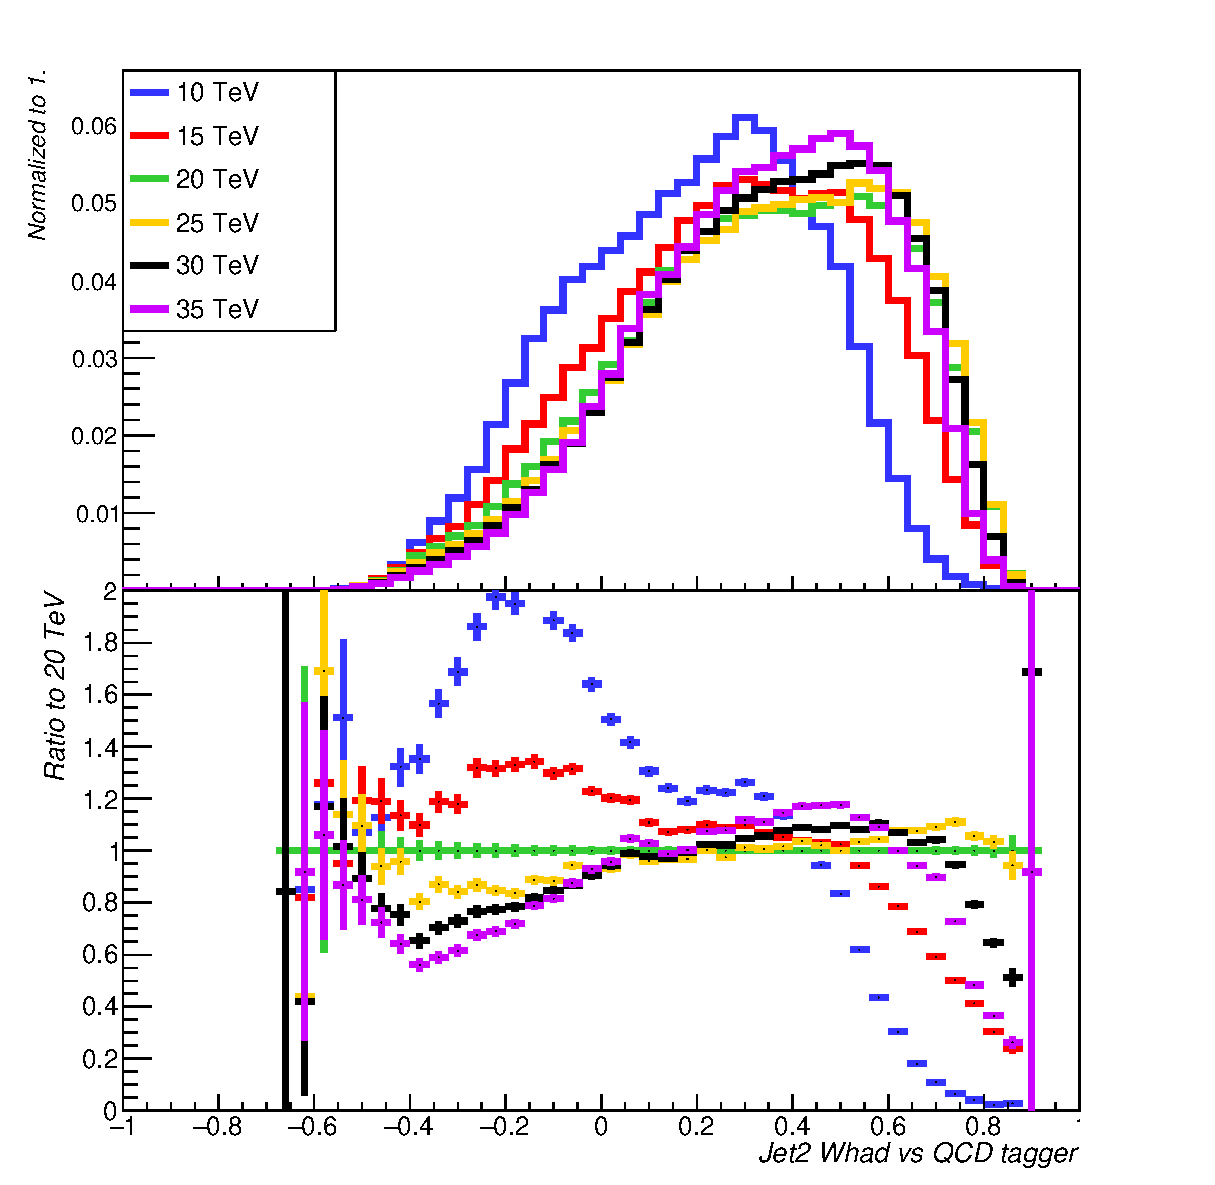
\includegraphics[width=0.495\textwidth]{Fig/TMVA/Jet2_Whad_vs_QCD_tagger.eps}
\caption{Signal BDT score shapes comparison for masses from 10 to 35 $\TeV$ (and ratio to 20 $\TeV$ mass) for leading jet (left) and second leading jet $\pt$ (right) for top Vs QCD tagger (top) and W Vs QCD tagger (bottom).}
\label{fig:BDT_signal_shape_comparison}
\end{figure}

\clearpage
\newpage

%%%%%%%%%%%%%%%%%%%%%%%%%%%%%%%%%%%%%%%%%%%%%%%%%%%%%
\subsection{Tag Rate Function}
\label{subsec:trf}
get annexe from Clement and copy it here.

%%%%%%%%%%%%%%%%%%%%%%%%%%%%%%%%%%%%%%%%%%%%%%%%%%%%%
\subsection{Limit settings}
\label{subsec:limitsettings}


%%%%%%%%%%%%%%%%%%%%%%%%%%%%%%%%%%%%%%%%%%%%%%%%%%%%%
%%%%%%%%%%%%%%%%%%%%%%%%%%%%%%%%%%%%%%%%%%%%%%%%%%%%%
\section{Physics models}
\label{sec:physmodel}

Models with extended gauge groups often feature additional U(1) symmetries with corresponding heavy spin-1 bosons. These bosons, generally referred to as $\Zp$, would manifest as a narrow resonance through
its  decay,  in  the  dilepton  mass  spectrum.   
Among  these  models  are  those  inspired  by  Grand  Unified Theories, which are 
motivated by gauge unification or a restoration of the left–right symmetry violated
by the weak interaction. Examples are the $\Zp$
bosons of the E6 motivated [1, 2] theories as well as Minimal models [3].  
The Sequential Standard Model (SSM) [2] posits a $\ZpSSM$ boson with couplings to fermions
that are identical to those of the SM $\Z$ boson. This model is a good benchmark as the 
results can be interpreted in the context of other models of new physics, and is useful 
for comparing the sensitivity of different experiments.



%%%%%%%%%%%%%%%%%%%%%%%%%%%%%%%%%%%%%%%%%%%%%%%%%%%%%
%%%%%%%%%%%%%%%%%%%%%%%%%%%%%%%%%%%%%%%%%%%%%%%%%%%%%
\section{Analyses at $100 TeV FCC-hh$}
\label{sec:ana100tev}

%%%%%%%%%%%%%%%%%%%%%%%%%%%%%%%%%%%%%%%%%%%%%%%%%%%%%
%%%%%%%%%%%%%%%%%%%%%%%%%%%%%%%%%%%%%%%%%%%%%%%%%%%%%
\subsection{Leptonic resonances : ee, $\mu\mu$, $\tau\tau$}
\label{subsec:lepreso}

%%%%%%%%%%%%%%%%%%%%%%%%%%%%%%%%%%%%%%%%%%%%%%%%%%%%%%%%%%%%%%%%%%%%%%%%%%%%%%%%%%%%%%%%%%%%
\subsubsection{Introduction}
Models with extended gauge groups often feature additional U(1) symmetries with corresponding heavy spin-1 bosons. These bosons, generally referred to as $\Zp$, would manifest themselves as a narrow resonance in the dilepton mass spectrum. Among these models are those inspired by Grand Unified Theories, motivated by gauge unification or a restoration of the left-right symmetry violated by the weak interaction. Examples include the $\Zp$ bosons of the E6 motivated theories~\cite{London:1986jz,Joglekar:2016yap,Langacker:2008yv} and Minimal models~\cite{Salvioni:2009mt}. The Sequential Standard Model (SSM)~\cite{Langacker:2008yv} posits a $\ZpSSM$ boson with couplings to fermions that are identical to those of the Standard Model $\Z$ boson.

The decay products of heavy resonances are in the multi-TeV regime and the capability to reconstruct their momentum imposes stringent requirement on the detector design. In particular, reconstructing the track curvature of multi-TeV muons requires excellent position resolution and a large lever arm. In this section, the expected sensitivity is presented for a \Zpll\ (where $\ell=\mathrm{e},\mu$) and \Zptata\ separately.

%%%%%%%%%%%%%%%%%%%%%%%%%%%%%%%%%%%%%%%%%%%%%%%%%%%%%%%%%%%%%%%%%%%%%%%%%%%%%%%%%%%%%%%%%%%%
\subsubsection{Monte Carlo Samples}
Monte Carlo~(MC) simulated event samples were used to simulate the response of the FCC detector to signal and backgrounds. The muon momentum resolution is assumed to be $\sigma(p)/p \approx 20\%$ at $\pt= 20 $TeV. Signals are generated with {\scshape Pythia}~8.230~\cite{Sjostrand:2014zea} using the leading order cross-section from the generator.
All lepton flavour decays of the $\ZpSSM$ are generated assuming universality of the couplings.
The Drell-Yan background has been generated using {\scshape MG5\_}a{\scshape MC@NLO}~2.5.2~\cite{Alwall:2014} at leading order only. A k-factor of 2 is applied to all the background processes.

%%%%%%%%%%%%%%%%%%%%%%%%%%%%%%%%%%%%%%%%%%%%%%%%%%%%%%%%%%%%%%%%%%%%%%%%%%%%%%%%%%%%%%%%%%%%
\subsubsection{Event Selection}
Events are required to contain two leptons with $\pt > 1$~TeV, $|\eta|$<4 and an invariant mass $\mll > 2.5$~TeV. For di-$\tau$ final state we focus on the most sensitive fully hadronic channel only. The di-$\tau$ event selection requires two jets with $p_{T} > 0.5$>~TeV and $|\eta|<2.5$ identified as $\tau$'s. To ensure no overlap between the $\ell$ and $\tau$ final states, jets containing leptons with $\pt > 100$~GeV are vetoed. Finally, requirements of $\Delta \phi(\tau_1, \tau_2)> 2$ and $2.5<\Delta R(\tau_1, \tau_2)<4$ are applied.
Mass dependent cuts applied to maximise the signal to background ratio are summarised in Table~\ref{tab:leptonicresonances:selectiontautau}.

Figure~\ref{figure:leptonicresonances:masses} (left and center) shows the invariant mass for a 30~TeV signal for the $ee$ and $\mu\mu$ channels, and the yields can be found in Table~\ref{tab:leptonicresonances:yieldstautau}. The mass resolution is better for the ee channel, as expected. Figure~\ref{figure:leptonicresonances:masses} (right) shows the transverse mass~\footnote{the transverse mass is defined as $m_{T}  =  \sqrt{2\ptZp*\met*(1-cos\Delta\phi(\Zp,\met))} $}
of a 10~TeV signal for the $\tau\tau$ channel, and the yields can be found in Table~\ref{tab:leptonicresonances:yieldsll}.
Several proxies for the true resonance mass have been tested, such as the invariant mass of the two taus, with and without correction for the missing energy. The transverse mass provided the best sensitivity and was therefore used to set limits and determine the discovery reach.

\begin{table}[htbp]
   \centering
\begin{tabular}{l|l|c|r}
   $\Zp$ mass [TeV] &  $\Delta \phi(\tau_1, \tau_2)$&  $\Delta R(\tau_1, \tau_2)$ & $\met$\\
  \hline
  $4-8$ & > 2.4 & > 2.5 and < 3.5 & > 400 GeV\\
  $10$ & > 2.4 & > 2.7 and < 4 & > 300 GeV\\
  $12-14$ & > 2.6 & > 2.7 and < 4 & > 300 GeV\\
  $16-18$ & > 2.7 & > 2.7 and < 4 & > 300 GeV\\
  $>18$ & > 2.8 & > 3 and < 4 & > 300 GeV\\
  \end{tabular}
  \caption{List of mass dependent cuts optimised to maximise the sensitivity for the \Zptata\ search.}
  \label{tab:leptonicresonances:selectiontautau}
\end{table}

\begin{table}[htbp]
   \centering
\begin{tabular}{l|r|r}
 & ee & $\mu\mu$  \\
  \hline
  Drell-Yan & 206882.9 & 236597.9 \\
  \hline
  $\Zp$ 4~TeV & 1421357.9    & 1598969.4 \\
  $\Zp$ 6~TeV & 349922.4  & 393117.6\\
  $\Zp$ 8~TeV &   115043.5 & 129698.7 \\
  $\Zp$ 10~TeV &  45423.5 & 50873.3 \\
  $\Zp$ 20~TeV &  1192.3 & 1411.5\\
  $\Zp$ 30~TeV &  88.2 & 107.6\\
  $\Zp$ 40~TeV &  11.7 & 14.1 \\
  $\Zp$ 50~TeV &  3.2 & 3.7\\
\end{tabular}
  \caption{Expected number of events for the \Zpee\ and \Zpmumu\ analysis after the full event selection for the various \Zp\ mass hypotheses}
  \label{tab:leptonicresonances:yieldsll}
\end{table}

\begin{table}[htbp]
   \centering
\begin{tabular}{l| r |r|r}
$\Zp$ mass [TeV]  & signal &  Drell-Yan & Di-jet \\
  \hline
  $4$     &  51479.5 &  \multirow{3}{*}{5669.2} &   \multirow{3}{*}{875561.7} \\
  $6$     &  22294.3  & &\\
  $8$     &  9140.7  &  &\\
  \hline

  $10$      & 5398.8 & 9008.3 & 2040422.6 \\
  \hline

  $12$ &  2261.4&  \multirow{3}{*}{8946.8} &  \multirow{3}{*}{1982792.8}  \\
  $14$ &  1040.9&  &  \\
  \hline

  $16$ &  489.6&  \multirow{3}{*}{8826.3} &  \multirow{3}{*}{1915211.5} \\
  $18$ &  251.9&  &  \\
    \hline

  $20$    &  122.6& \multirow{3}{*}{7777.2} & \multirow{3}{*}{1609435.6}   \\
  $25$    &  27.5 &  &  \\
  $30$    &  7.1 &  &  \\
\end{tabular}
  \caption{Expected number of events for the \Zptata\ analysis after the full event selection for the various \Zp\ mass hypotheses}
  \label{tab:leptonicresonances:yieldstautau}
\end{table}

\begin{figure}
  \centering
  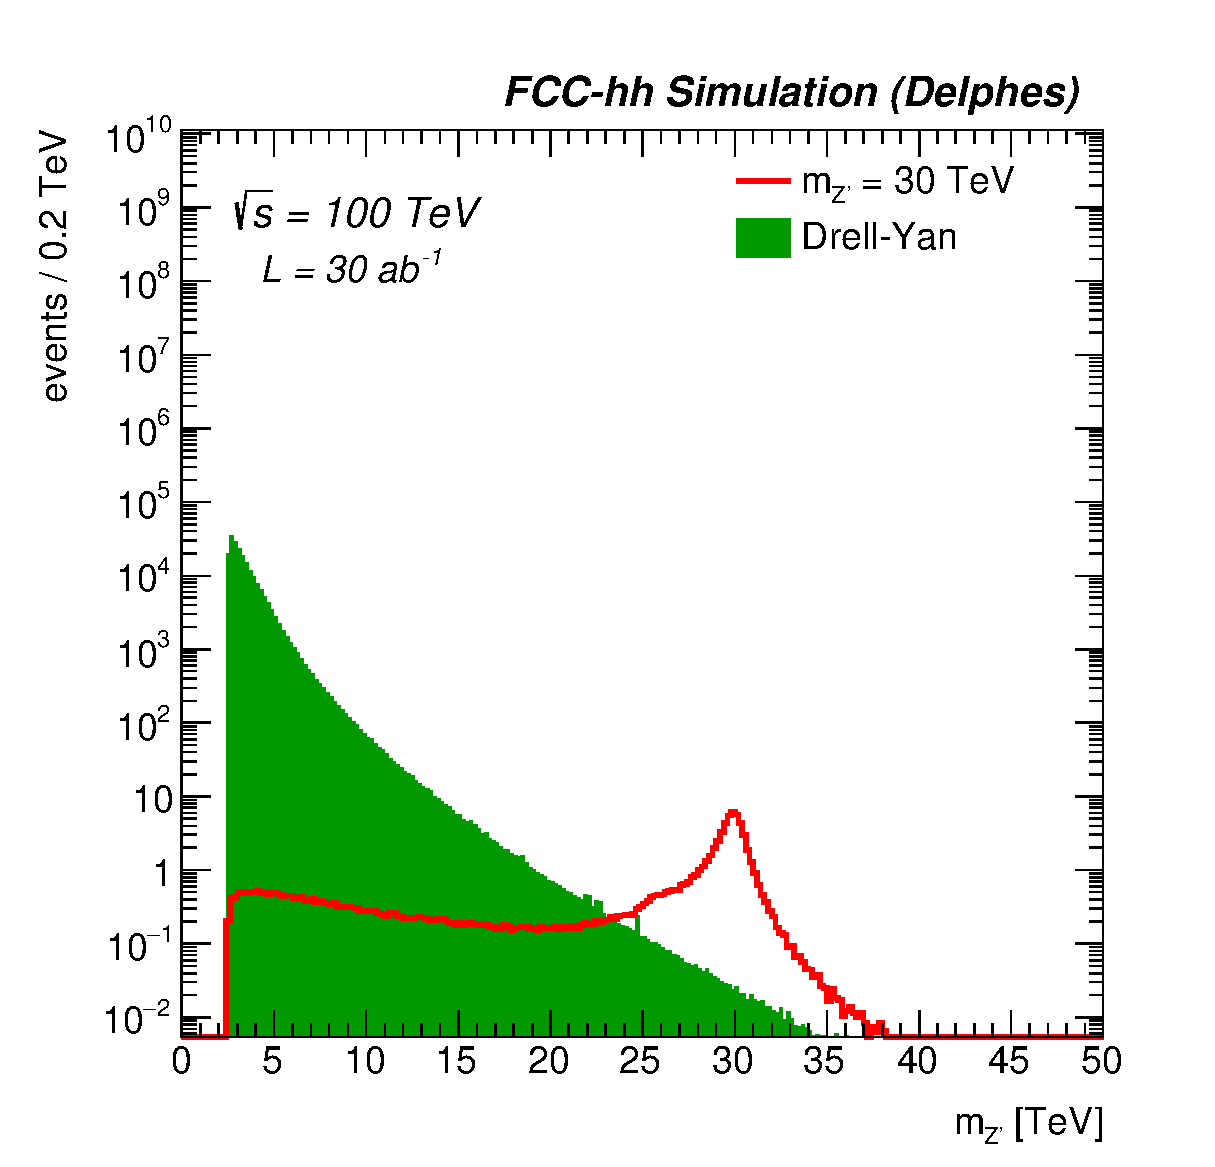
\includegraphics[width=0.30\columnwidth]{Fig/mzp_sel0_nostack_log_ee.eps}
  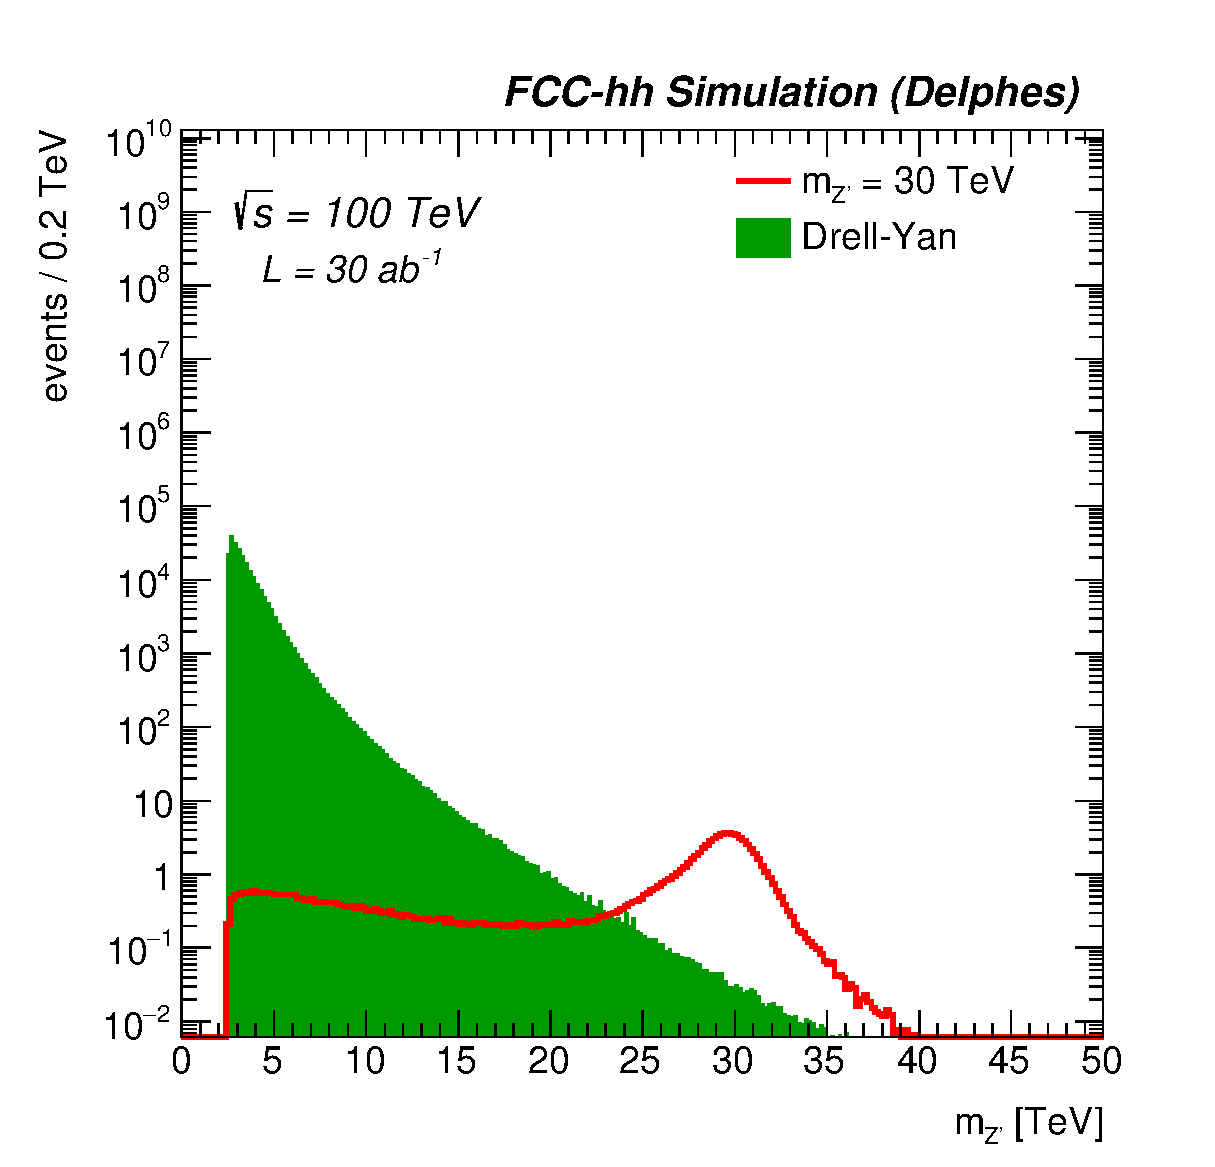
\includegraphics[width=0.30\columnwidth]{Fig/mzp_sel0_nostack_log_mm.eps}
  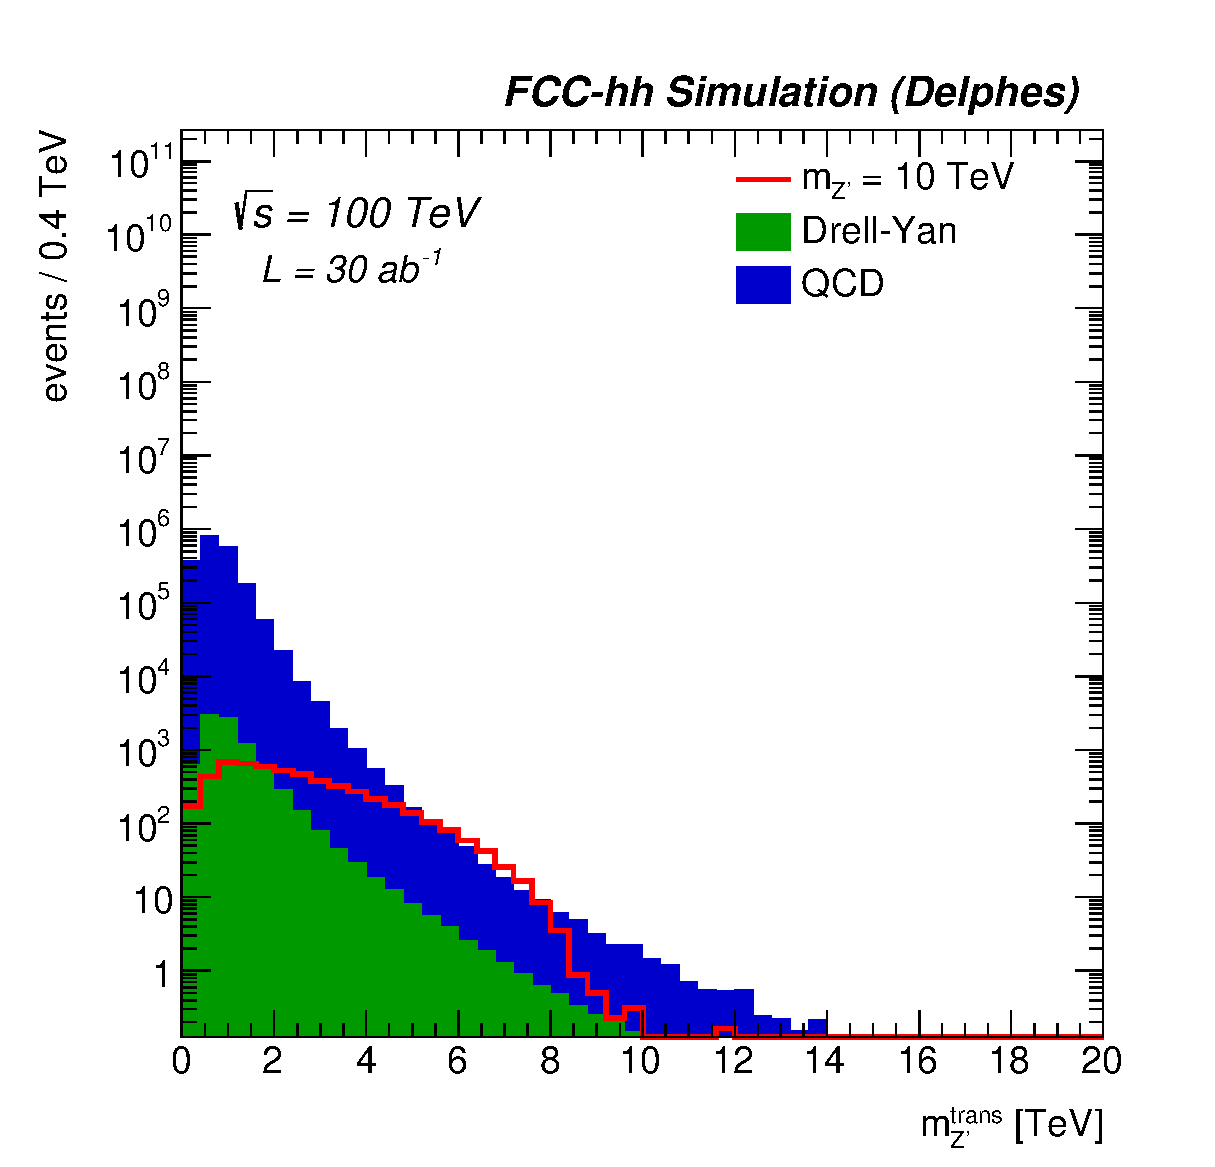
\includegraphics[width=0.30\columnwidth]{Fig/mt_finalsel_nostack_log.eps}
  \caption{Left, center: Invariant mass for a 30~TeV signal after full event selection for ee channel (left) and $\mu\mu$ channel (center). Right: Transverse mass for a 10~TeV signal after full event selection for the $\tau\tau$ channel. }
  \label{figure:leptonicresonances:masses}
\end{figure}
%\MS{need editing / style}

%%%%%%%%%%%%%%%%%%%%%%%%%%%%%%%%%%%%%%%%%%%%%%%%%%%%%%%%%%%%%%%%%%%%%%%%%%%%%%%%%%%%%%%%%%%%
\subsubsection{Results and discussion}
Hypothesis testing is performed using a modified frequentist method based on a profile likelihood that takes into account the systematic uncertainties as nuisance parameters that are fitted to the expected Monte-Carlo. For the $ee$ and $\mu\mu$ analyses, the di-lepton invariant mass is used as the discriminant, while for the $\tau\tau$ channel the transverse mass is used. A 50\% uncertainty on the background normalisation is assumed.

Figure~\ref{figure:leptonicresonances:resultsll} shows the exclusion limit obtained \intlumifcc\ of data for the ee alone (top left), $\mu\mu$ alone (top right) and combination of (ee,$\mu\mu$) channels (bottom left). Figure~\ref{figure:leptonicresonances:resultsll} (bottom right) shows the integrated luminosity required to reach a $5\sigma$ discovery for the leptonic resonances as a function of the mass of the heavy resonance. The \Zpee\ and \Zpmumu\ channel display very similar performance, due to the low background rates. We conclude therefore that the reference detector design features near to optimal performance for searches involving high \pT\ muon final states. Figure~\ref{figure:leptonicresonances:resultstautau} shows the exclusion limits for 30 ab$^{-1}$ of data (left) and the required integrated luminosity
versus mass to reach a $5\sigma$ discovery (right) for the di-tau resonances.

The discovery potential for high mass resonances decaying to $ee$, $\mu\mu$ and $\tau\tau$ has been studied using as a benchmark the \ZpSSM\ model. The very large centre of mass energy provides a correspondingly large mass reach. For the $ee$ and $\mu\mu$ cases masses up to 42~TeV can be excluded or discovered. Heavy resonance decaying to $\tau$ leptons reconstructed in the hadronic decay mode are more challenging, but we would be able to probe massses up to 18~TeV.

\begin{figure}
  \centering
  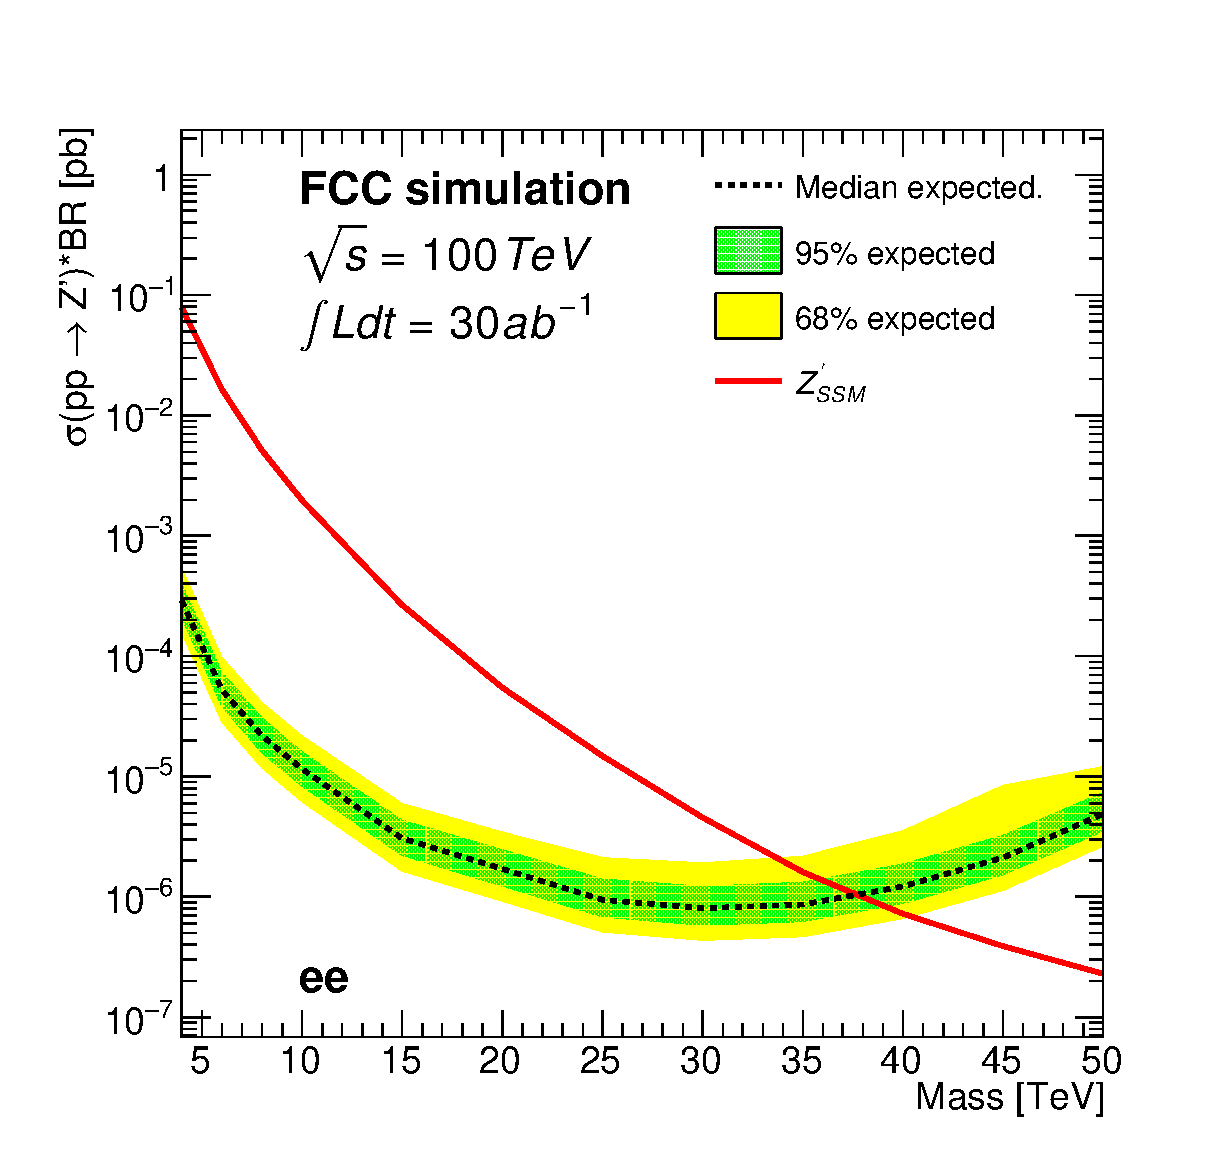
\includegraphics[width=0.45\columnwidth]{Fig/lim_Zprime_ee_fcc_v02.eps}
  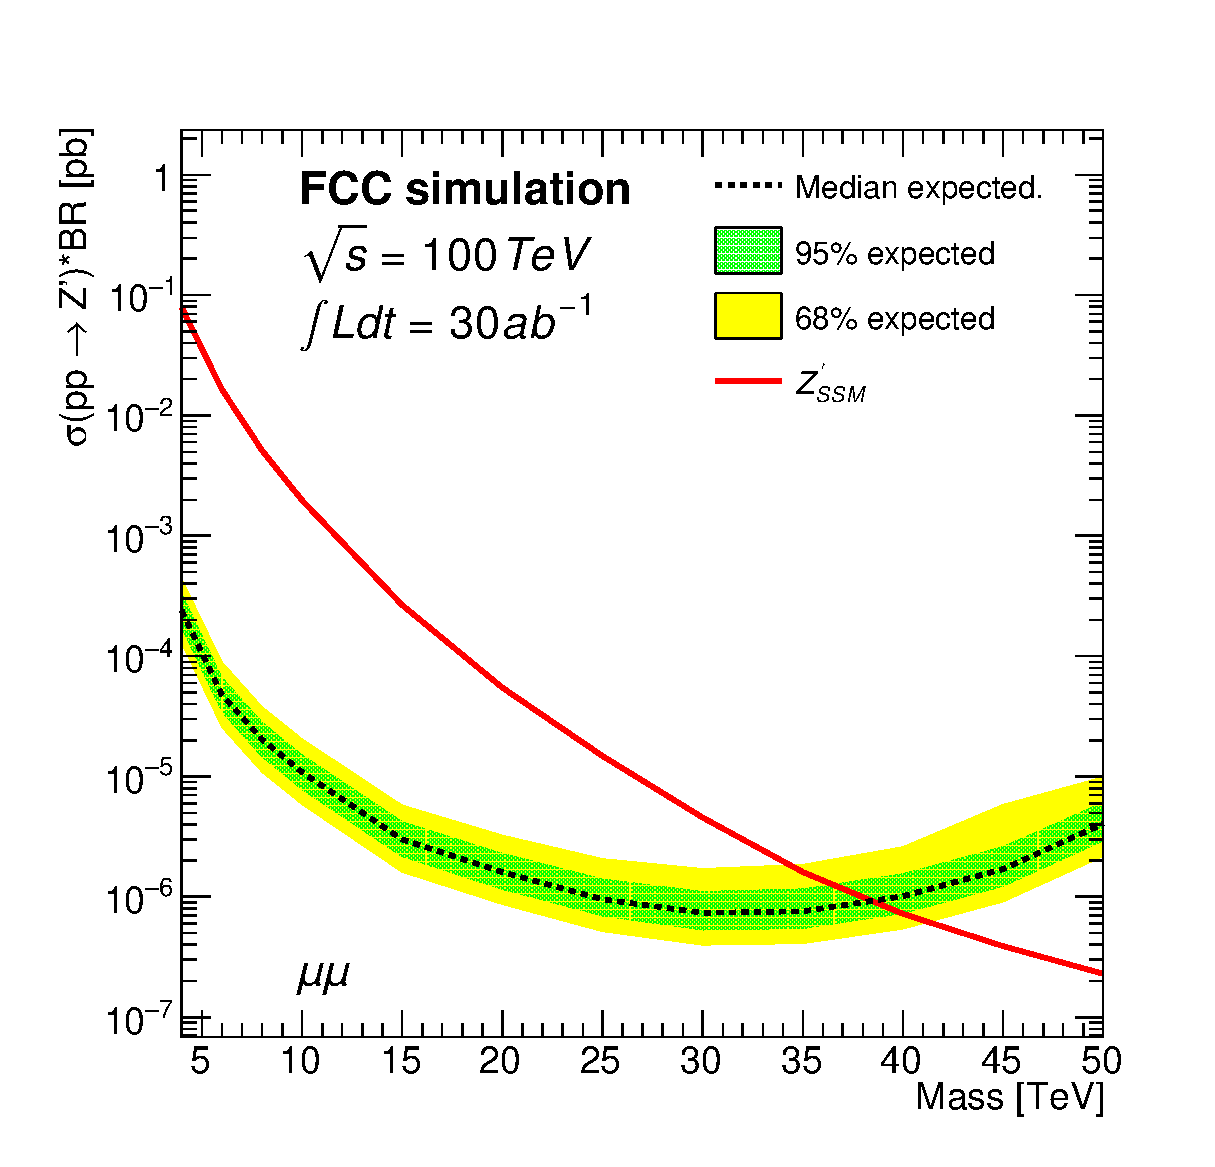
\includegraphics[width=0.45\columnwidth]{Fig/lim_Zprime_mumu_fcc_v02.eps}
  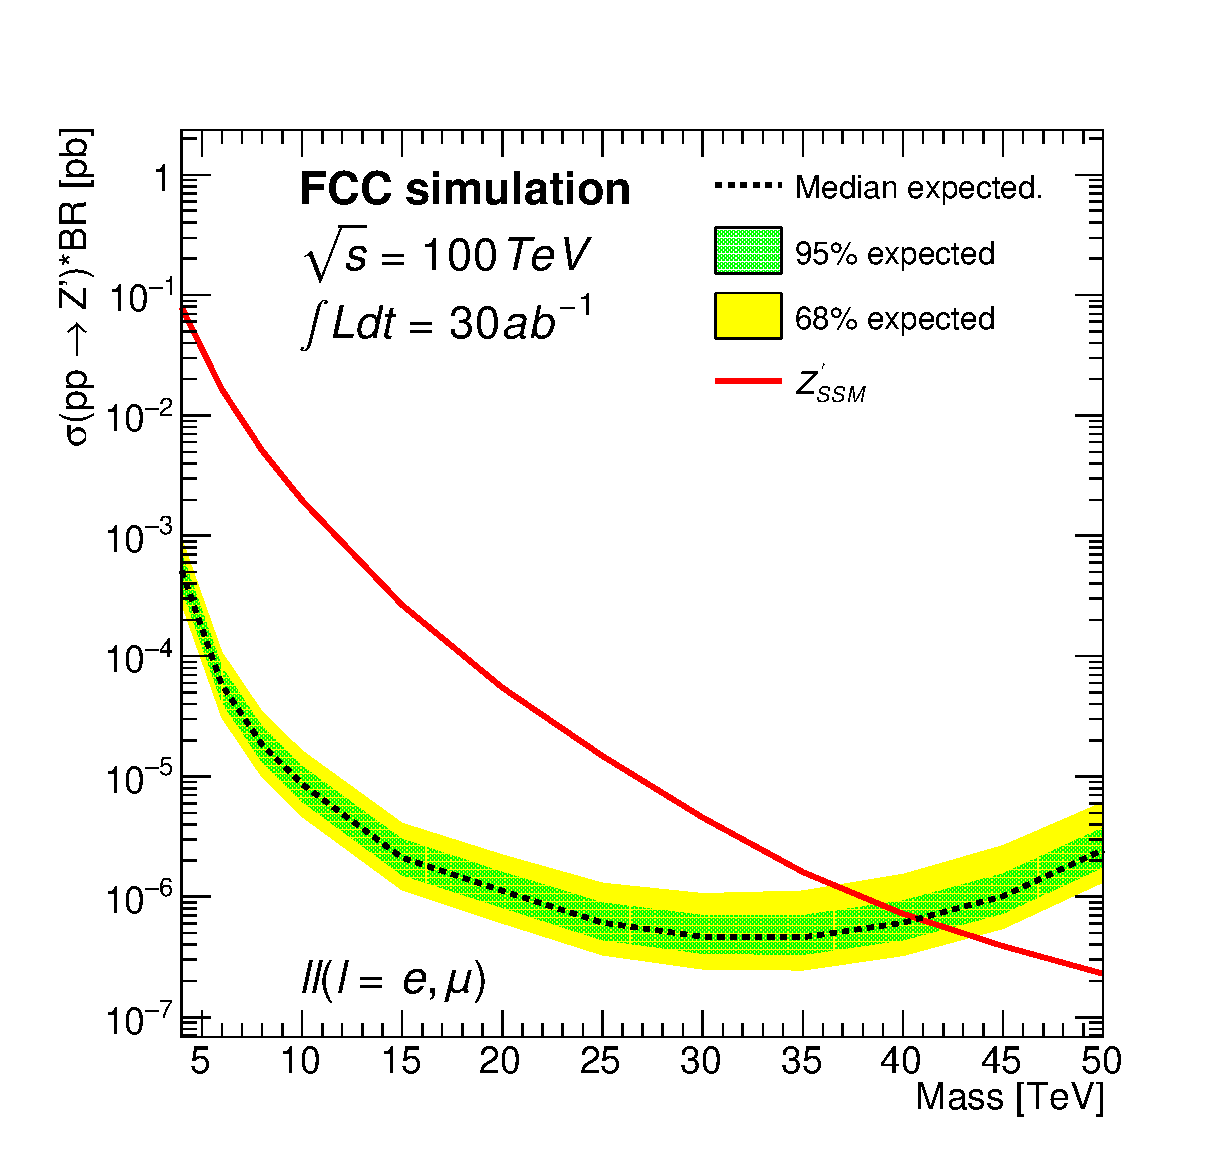
\includegraphics[width=0.45\columnwidth]{Fig/lim_Zprime_ll_fcc_v02.eps}
  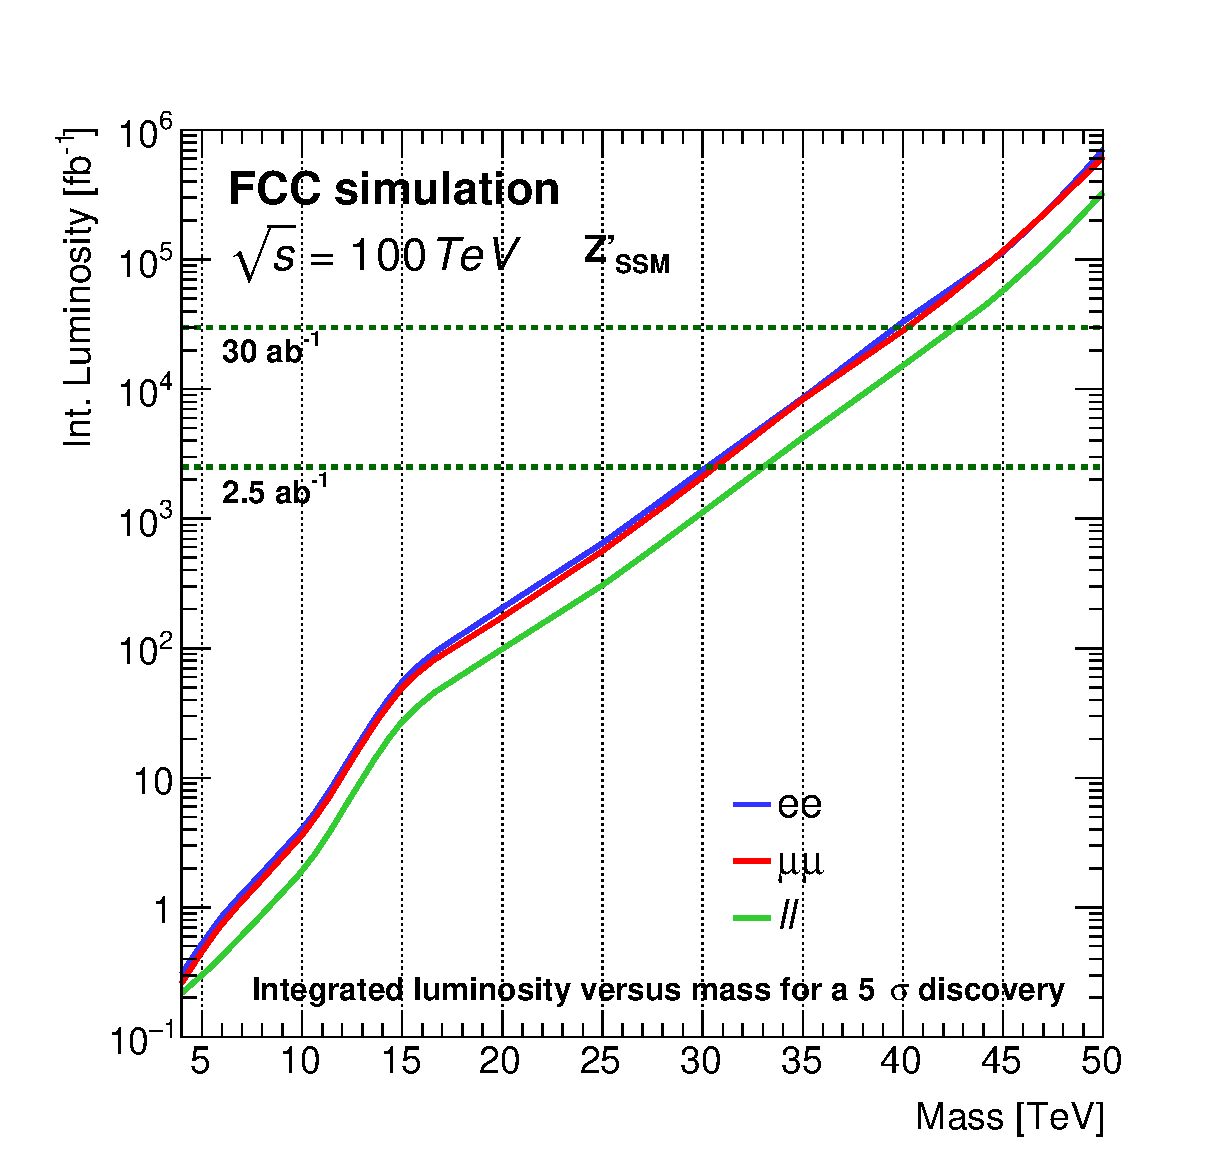
\includegraphics[width=0.45\columnwidth]{Fig/DiscoveryPotential_ll_comb_rootStyle.eps}
  \caption{Limit versus mass for the di-lepton (ee,$\mu\mu$) channel (left) and luminosity for a $5\sigma$ discovery (right) comparing ee,$\mu\mu$ and combined channels. }
  \label{figure:leptonicresonances:resultsll}
\end{figure}

\begin{figure}
  \centering
  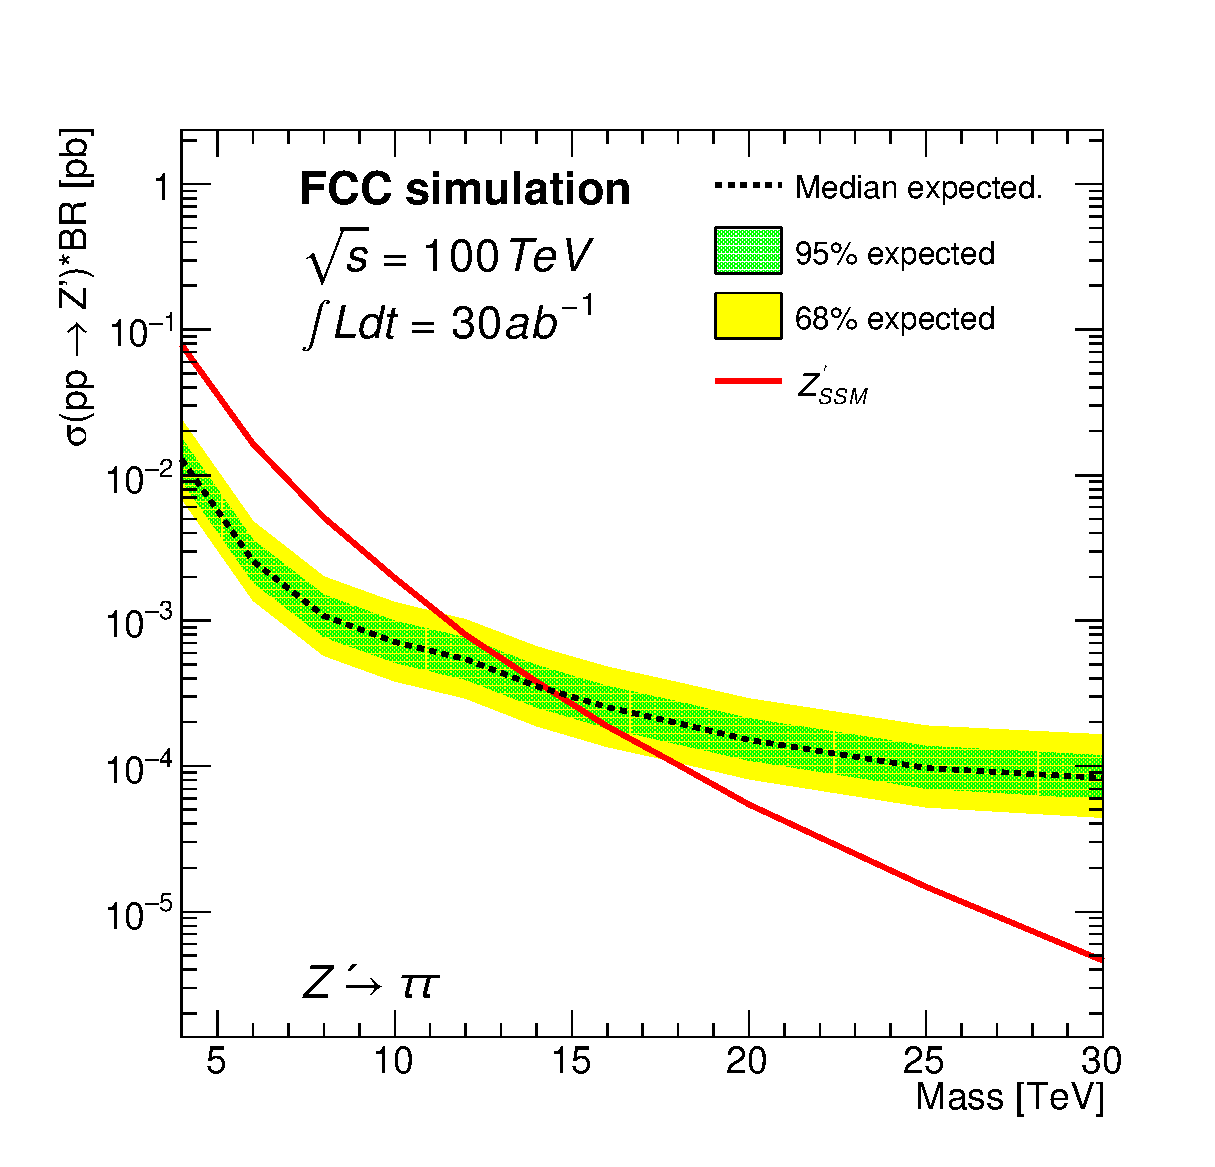
\includegraphics[width=0.45\columnwidth]{Fig/lim_Zprime_tautau_fcc_v02.eps}
    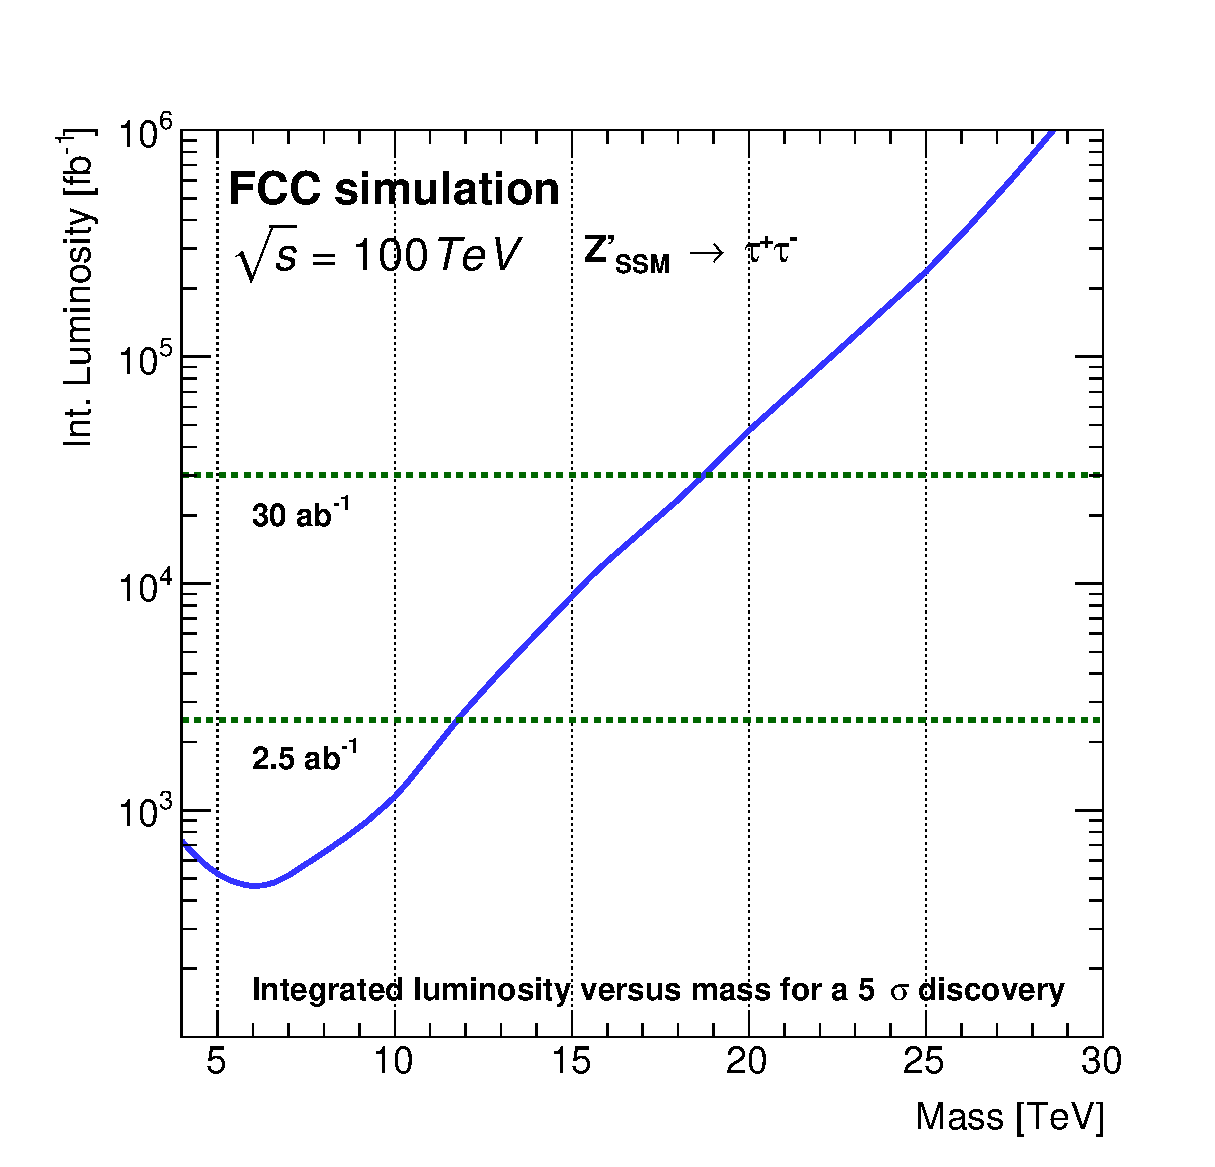
\includegraphics[width=0.45\columnwidth]{Fig/DiscoveryPotential_tautau_rootStyle.eps}
  \caption{Limit versus mass for the di-tau channel (left) and luminosity for a $5\sigma$ discovery (right). }
  \label{figure:leptonicresonances:resultstautau}
\end{figure}

\subsubsection{Flavour anomaly model}
few lines to explain same selection as Zprimemumu adn put plots for final sel+limit+disco

\begin{figure}
  \centering
  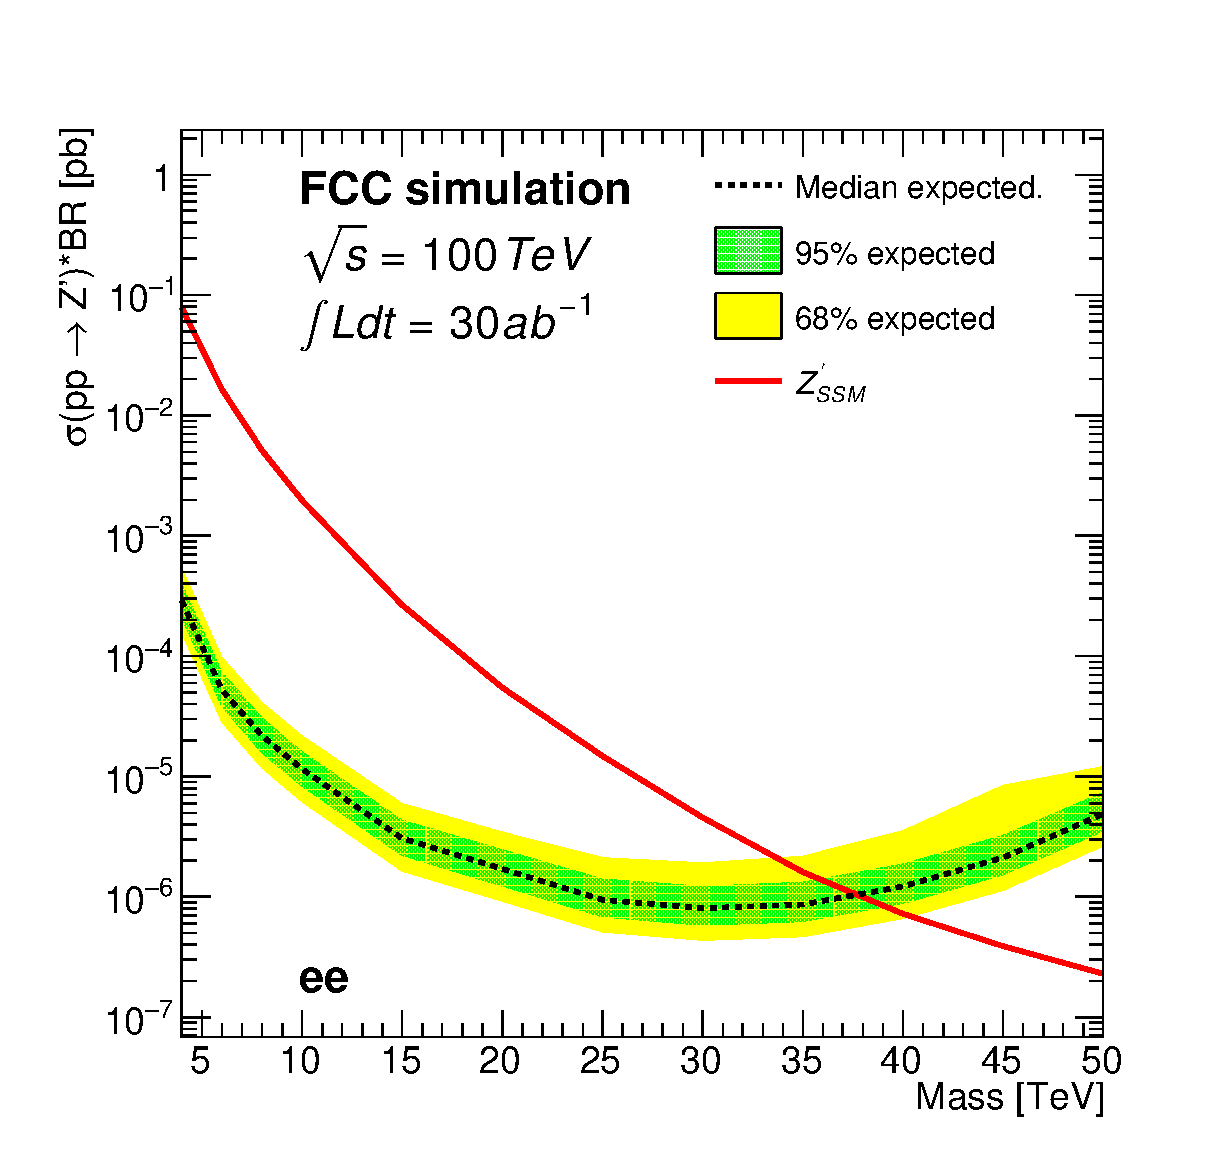
\includegraphics[width=0.45\columnwidth]{Fig/lim_Zprime_ee_fcc_v02.eps}
  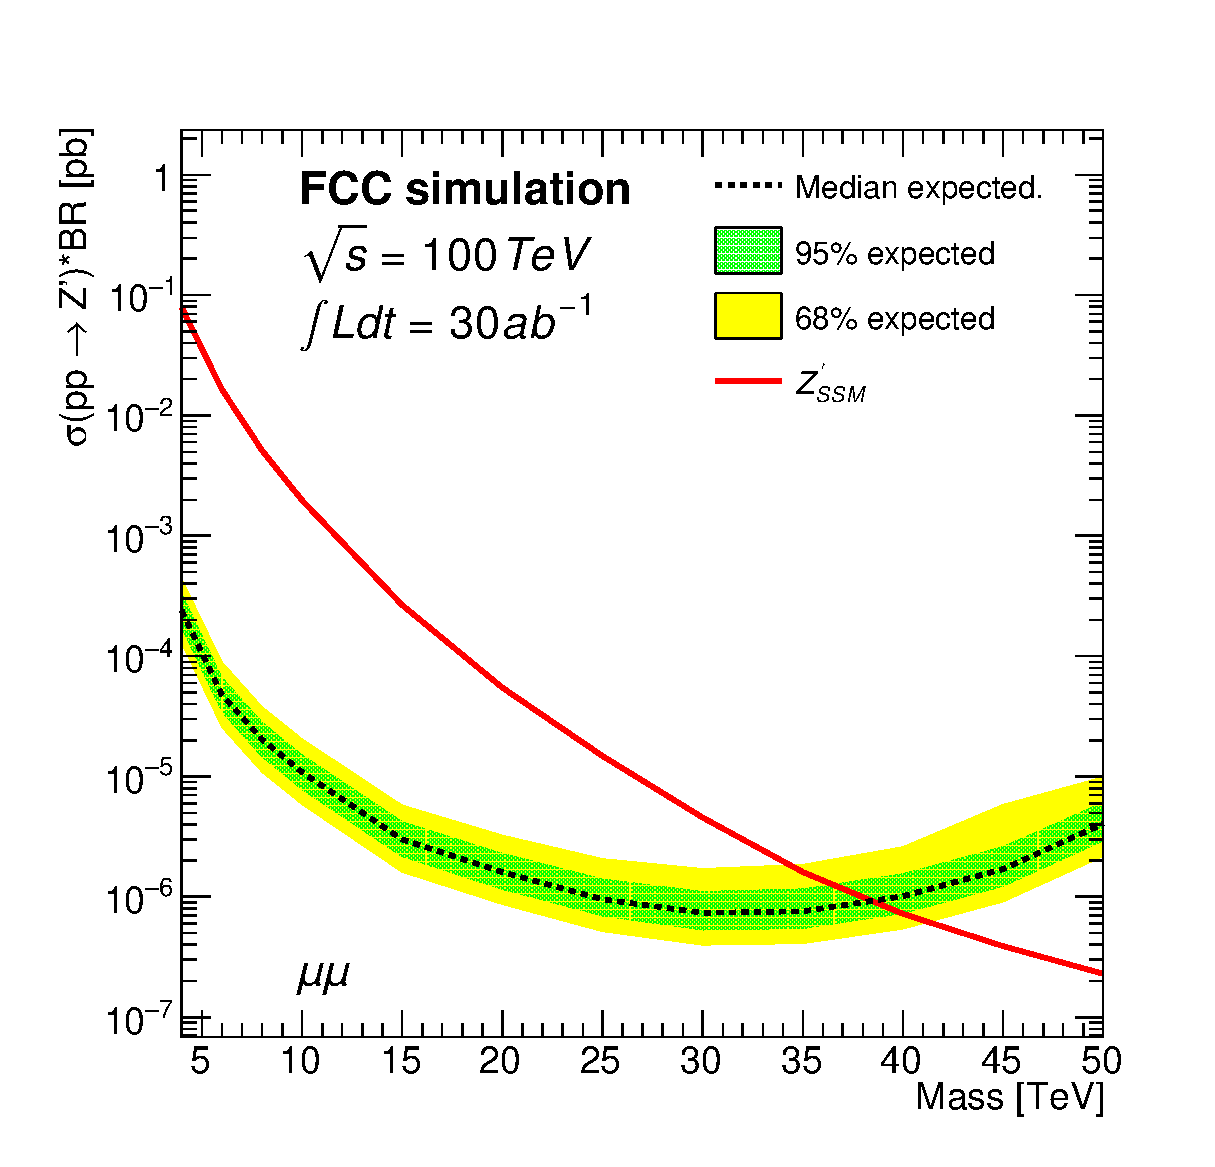
\includegraphics[width=0.45\columnwidth]{Fig/lim_Zprime_mumu_fcc_v02.eps}
  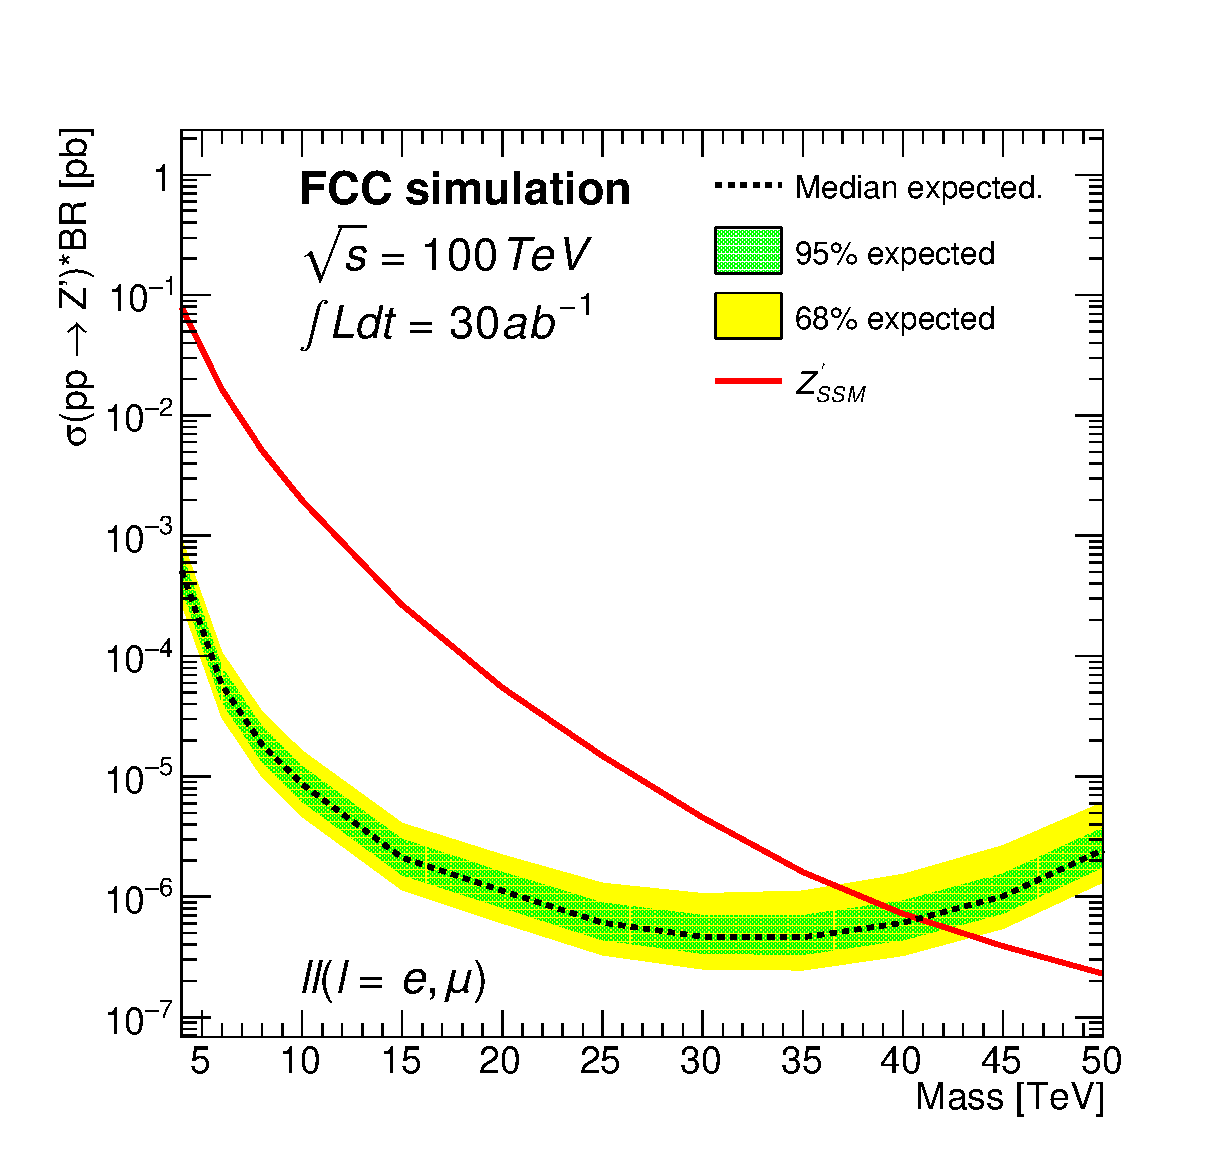
\includegraphics[width=0.45\columnwidth]{Fig/lim_Zprime_ll_fcc_v02.eps}
  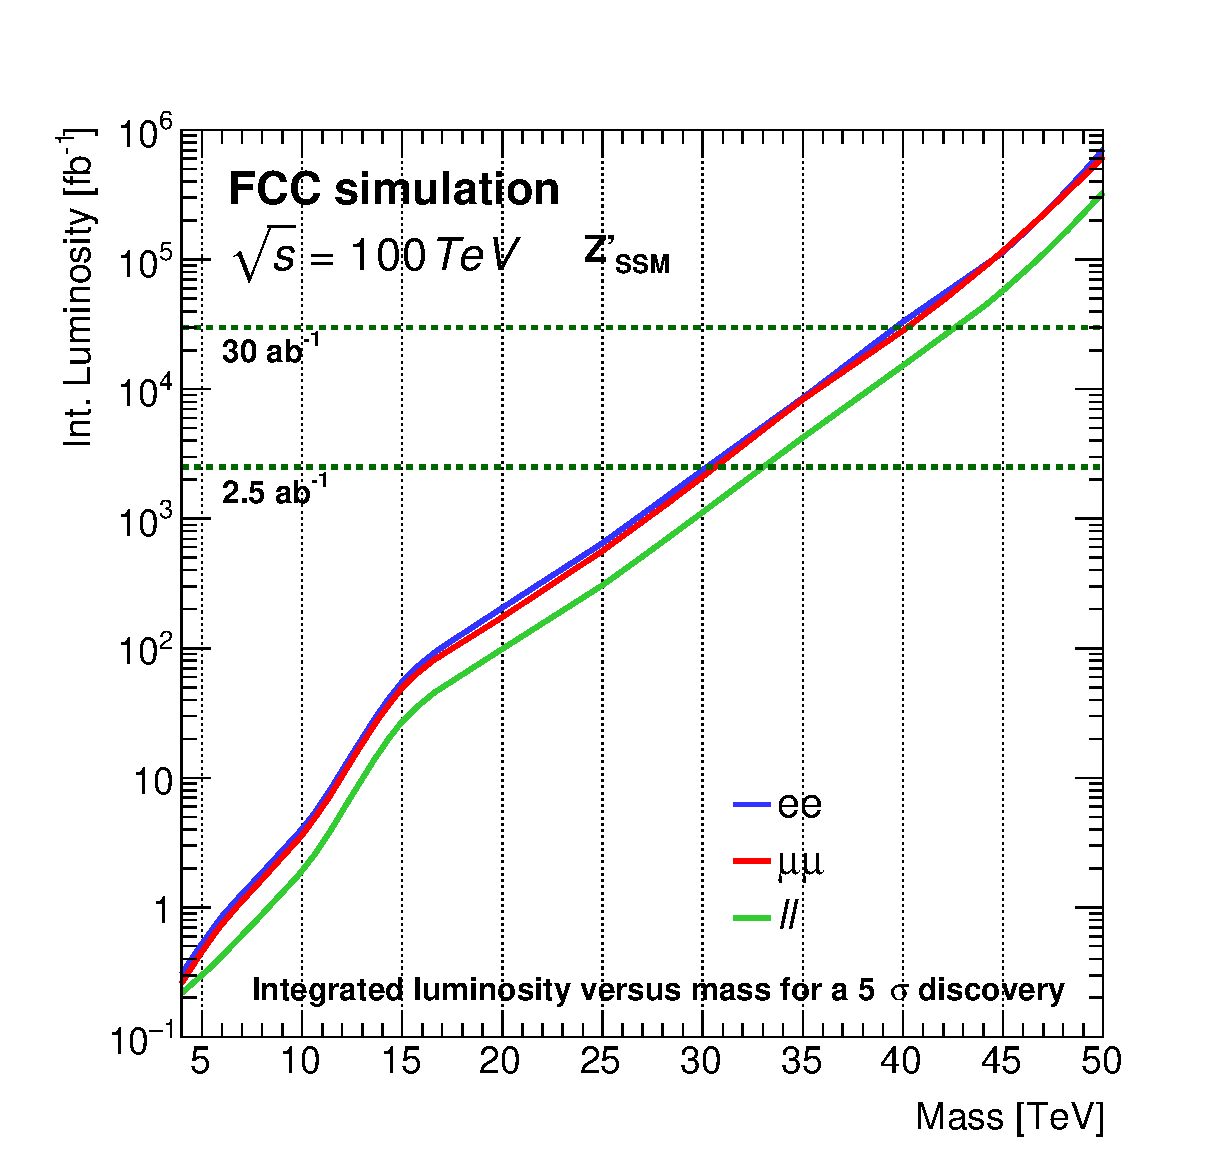
\includegraphics[width=0.45\columnwidth]{Fig/DiscoveryPotential_ll_comb_rootStyle.eps}
  \caption{Limit versus mass for the di-lepton (ee,$\mu\mu$) channel (left) and luminosity for a $5\sigma$ discovery (right) comparing ee,$\mu\mu$ and combined channels. }
  \label{figure:leptonicresonances:resultsll}
\end{figure}

%%%%%%%%%%%%%%%%%%%%%%%%%%%%%%%%%%%%%%%%%%%%%%%%%%%%%

% ll plots OLD
%\begin{figure}[!htb]\centering
%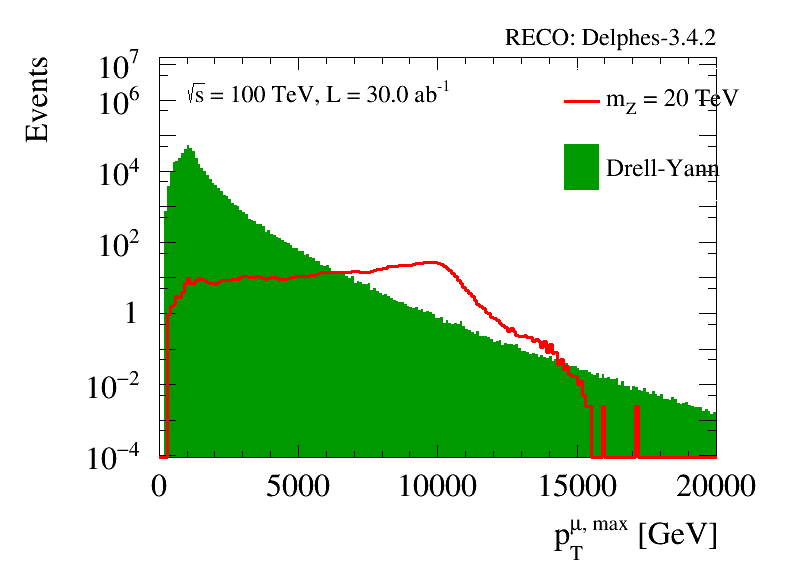
\includegraphics[width=0.495\textwidth]{Fig/FCC_ptmu_1_sel0_nostack_log.png}
%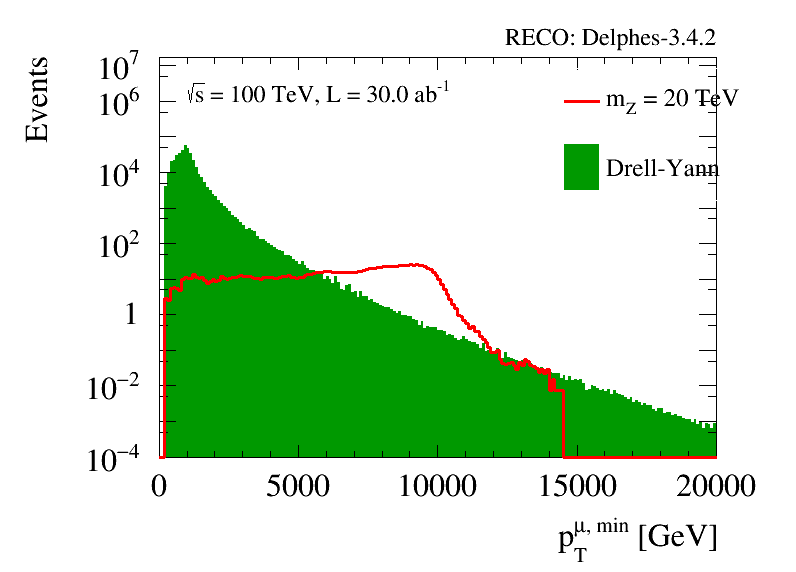
\includegraphics[width=0.495\textwidth]{Fig/FCC_ptmu_2_sel0_nostack_log.png}
%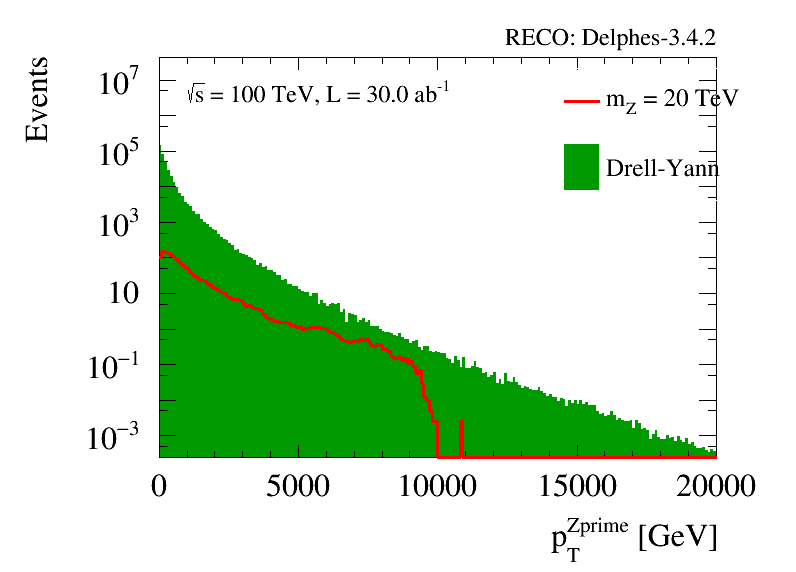
\includegraphics[width=0.495\textwidth]{Fig/FCC_ptzp_sel0_nostack_log.png}
%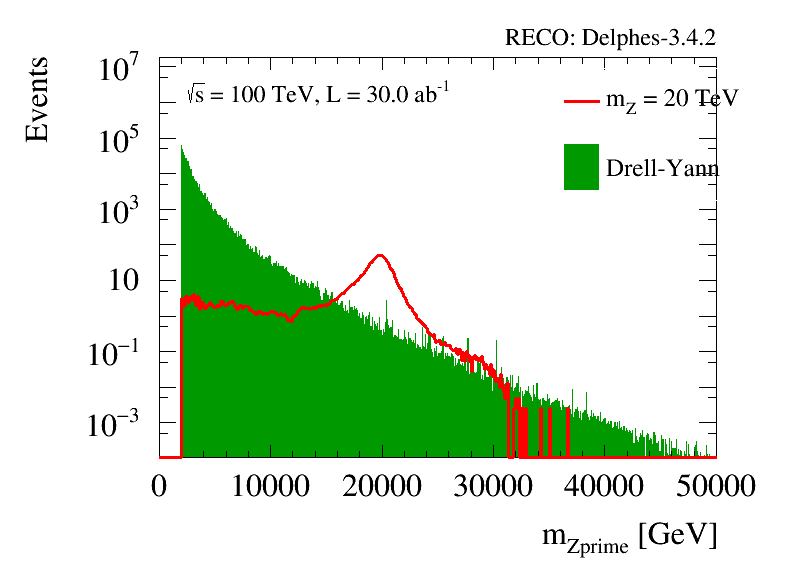
\includegraphics[width=0.495\textwidth]{Fig/FCC_mzp_sel0_nostack_log.png}
%\caption{Leading (top left) and sub-leading (top right) $\ptMu$, $\ptZp$ (bottom left) and 
%di-lepton invariant mass $\mll$ (bottom right) for the FCC 
%baseline detector}
%\label{fig:zpll_fcc}
%\end{figure}
%
%
%\begin{figure}[!htb]\centering
%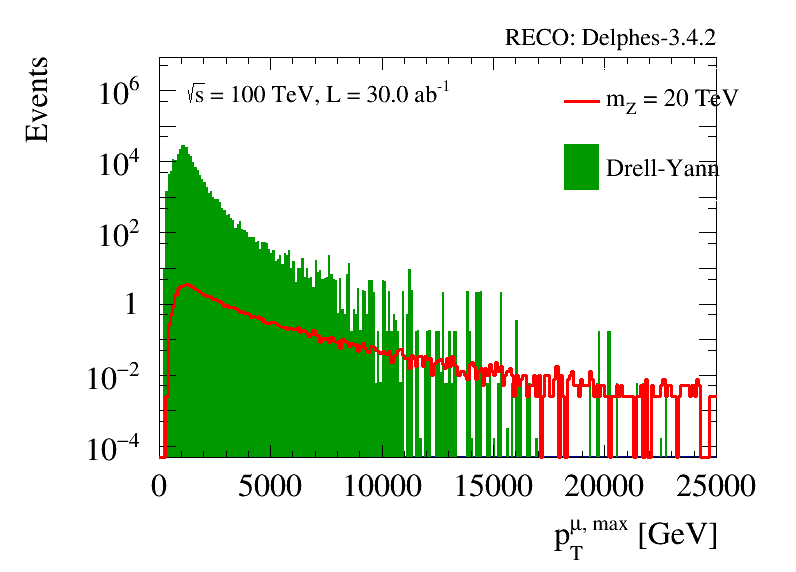
\includegraphics[width=0.495\textwidth]{Fig/CMS_ptmu_1_sel0_nostack_log.png}
%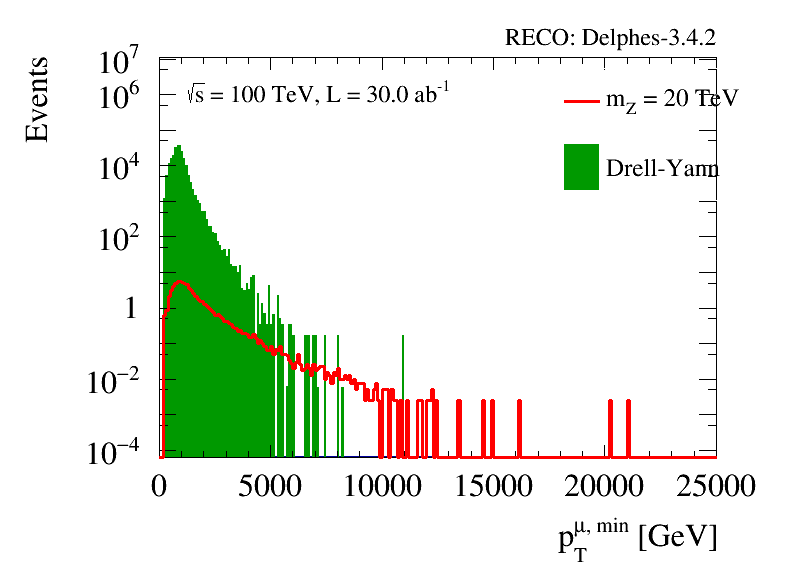
\includegraphics[width=0.495\textwidth]{Fig/CMS_ptmu_2_sel0_nostack_log.png}
%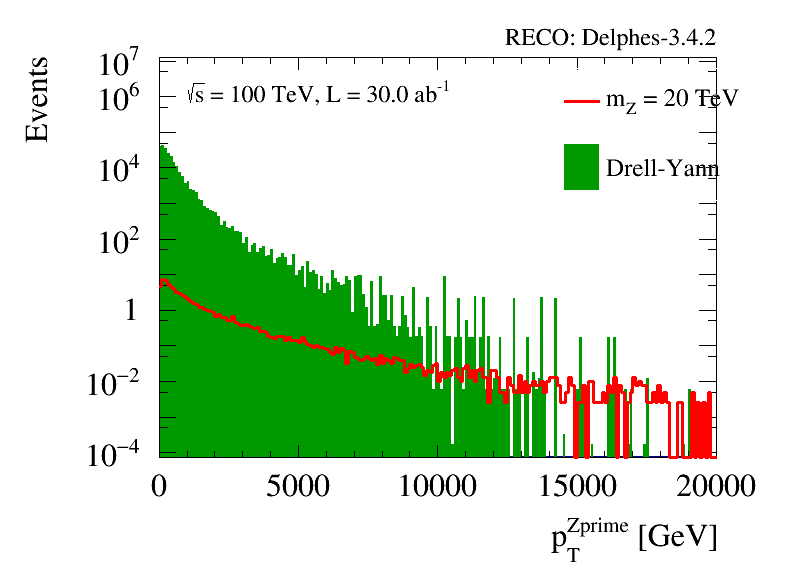
\includegraphics[width=0.495\textwidth]{Fig/CMS_ptzp_sel0_nostack_log.png}
%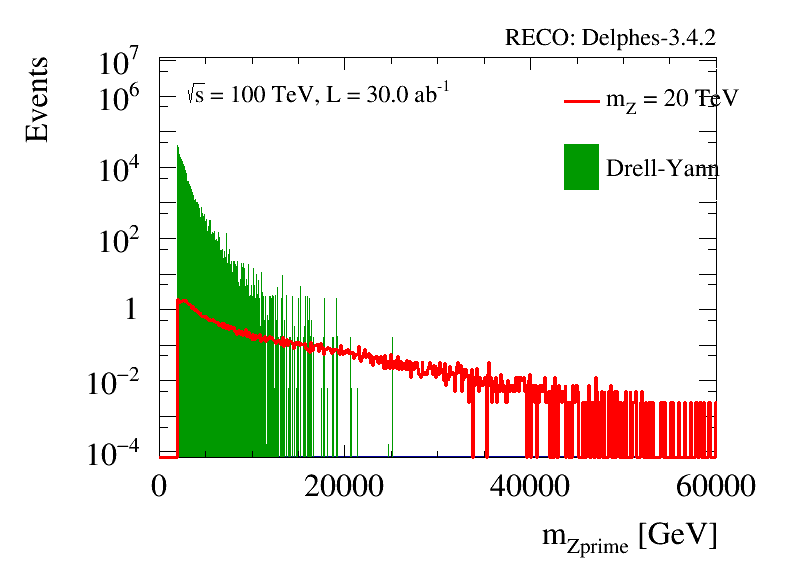
\includegraphics[width=0.495\textwidth]{Fig/CMS_mzp_sel0_nostack_log.png}
%\caption{Leading (top left) and sub-leading (top right) $\ptMu$, $\ptZp$ (bottom left) and 
%di-lepton invariant mass $\mll$ (bottom right) for the CMS  detector}
%\label{fig:zpll_cms}
%\end{figure}
%
%\begin{figure}[!htb]\centering
%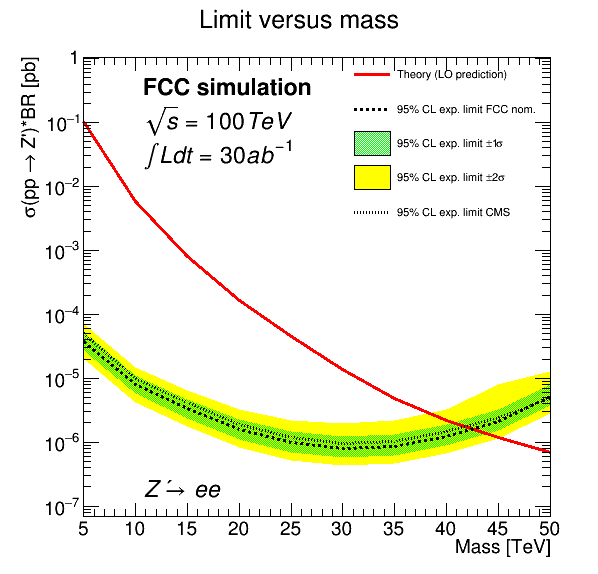
\includegraphics[width=0.495\textwidth]{Fig/lim_Zprime_ee_fcc_cms.png}
%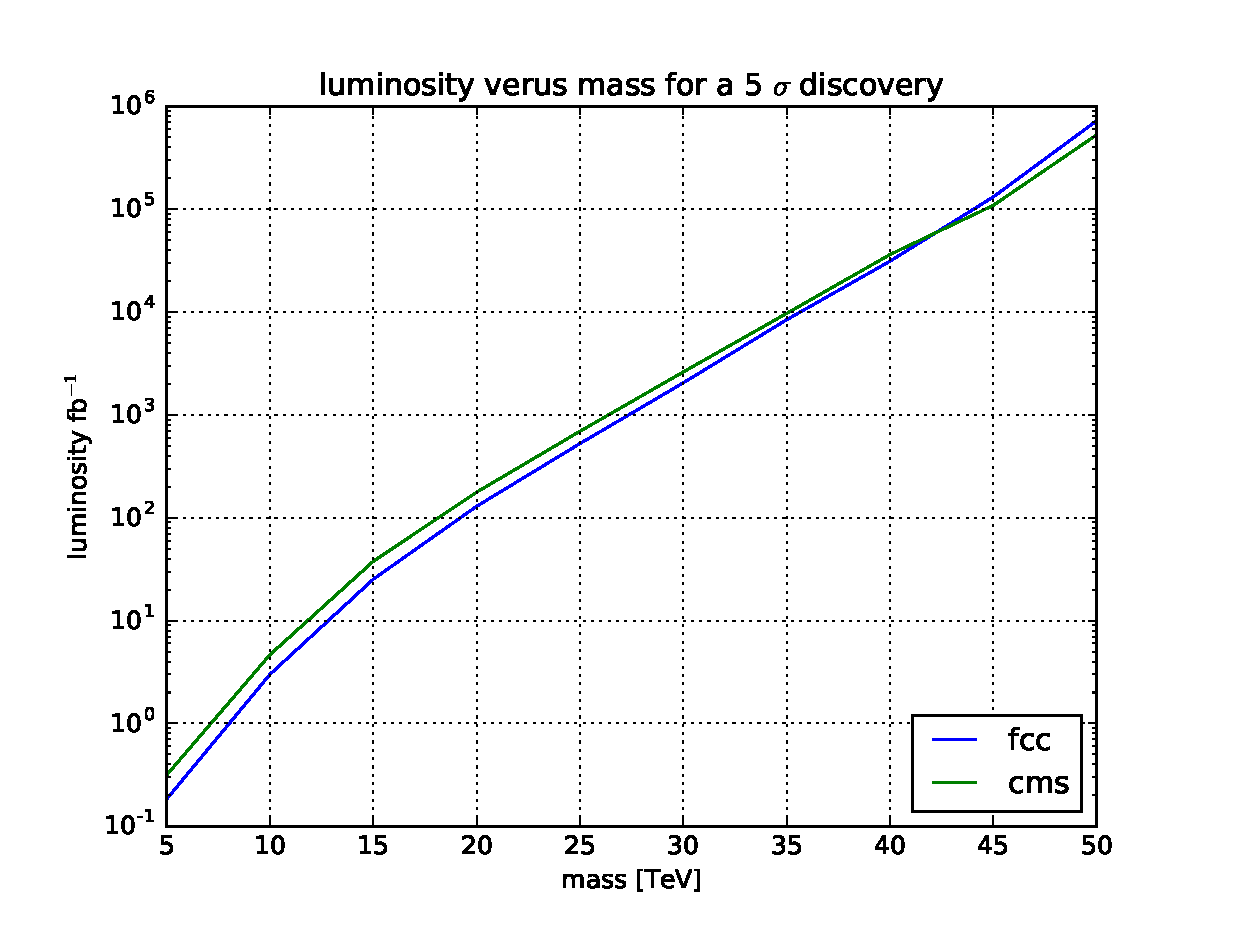
\includegraphics[width=0.495\textwidth]{Fig/DiscoveryPotential_ee.eps}
%\caption{Limit versus mass (left) and luminosity for a $5\sigma$ discovery (right) for the
% di-electron channel.}
%\label{fig:zpee_lim}
%\end{figure}
%
%\begin{figure}[!htb]\centering
%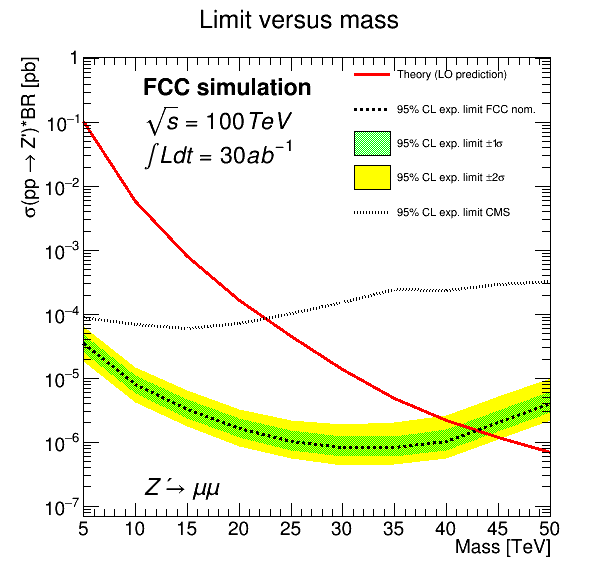
\includegraphics[width=0.495\textwidth]{Fig/lim_Zprime_mumu_fcc_cms.png}
%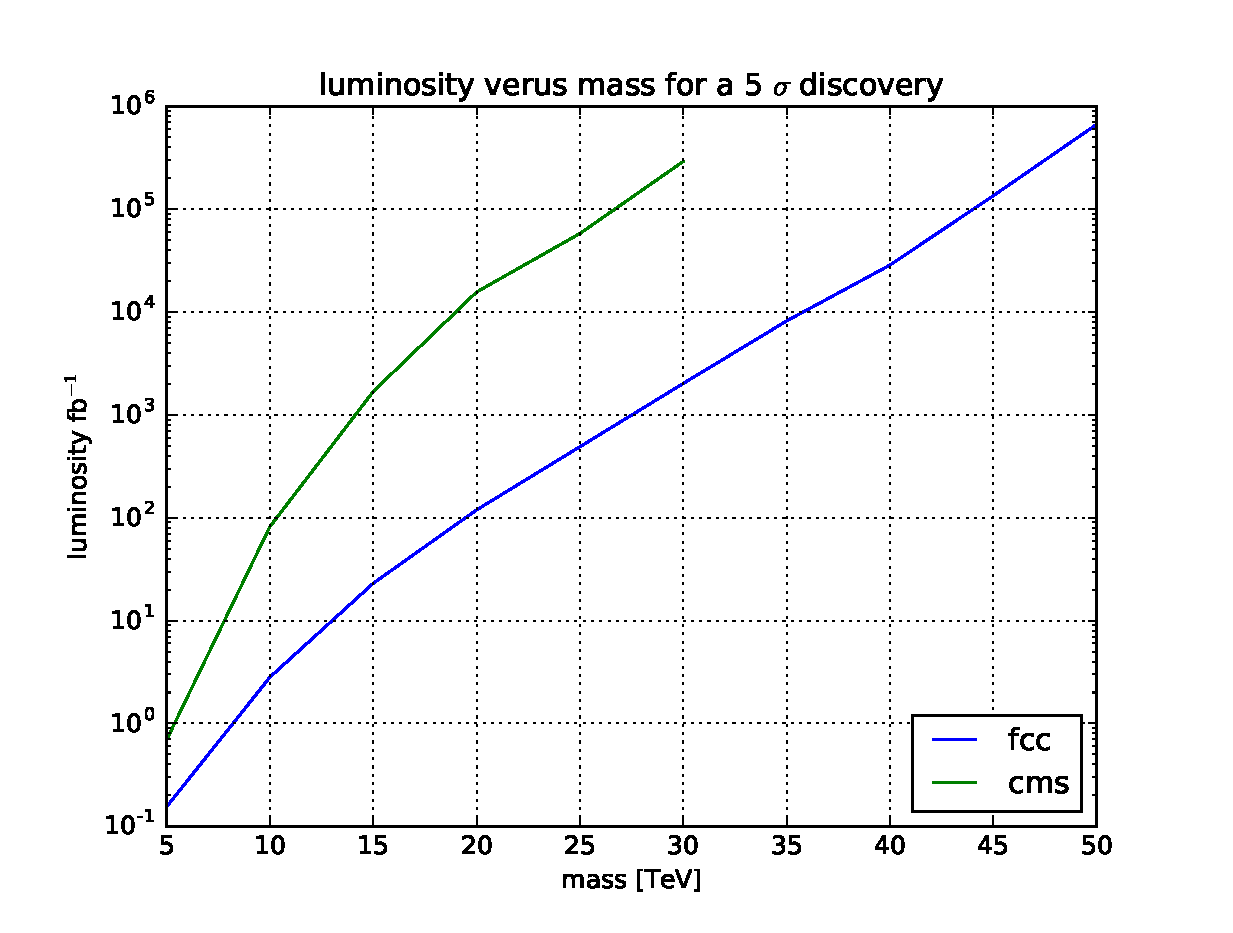
\includegraphics[width=0.495\textwidth]{Fig/DiscoveryPotential_mumu.eps}
%\caption{Limit versus mass (left) and luminosity for a $5\sigma$ discovery (right) for the
% di-muon channel.}
%\label{fig:zpmumu_lim}
%\end{figure}
%
%\begin{figure}[!htb]\centering
%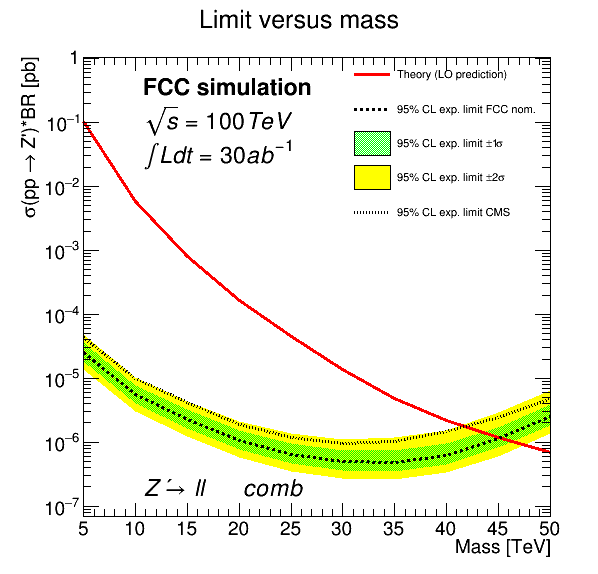
\includegraphics[width=0.495\textwidth]{Fig/lim_Zprime_ll_fcc_cms.png}
%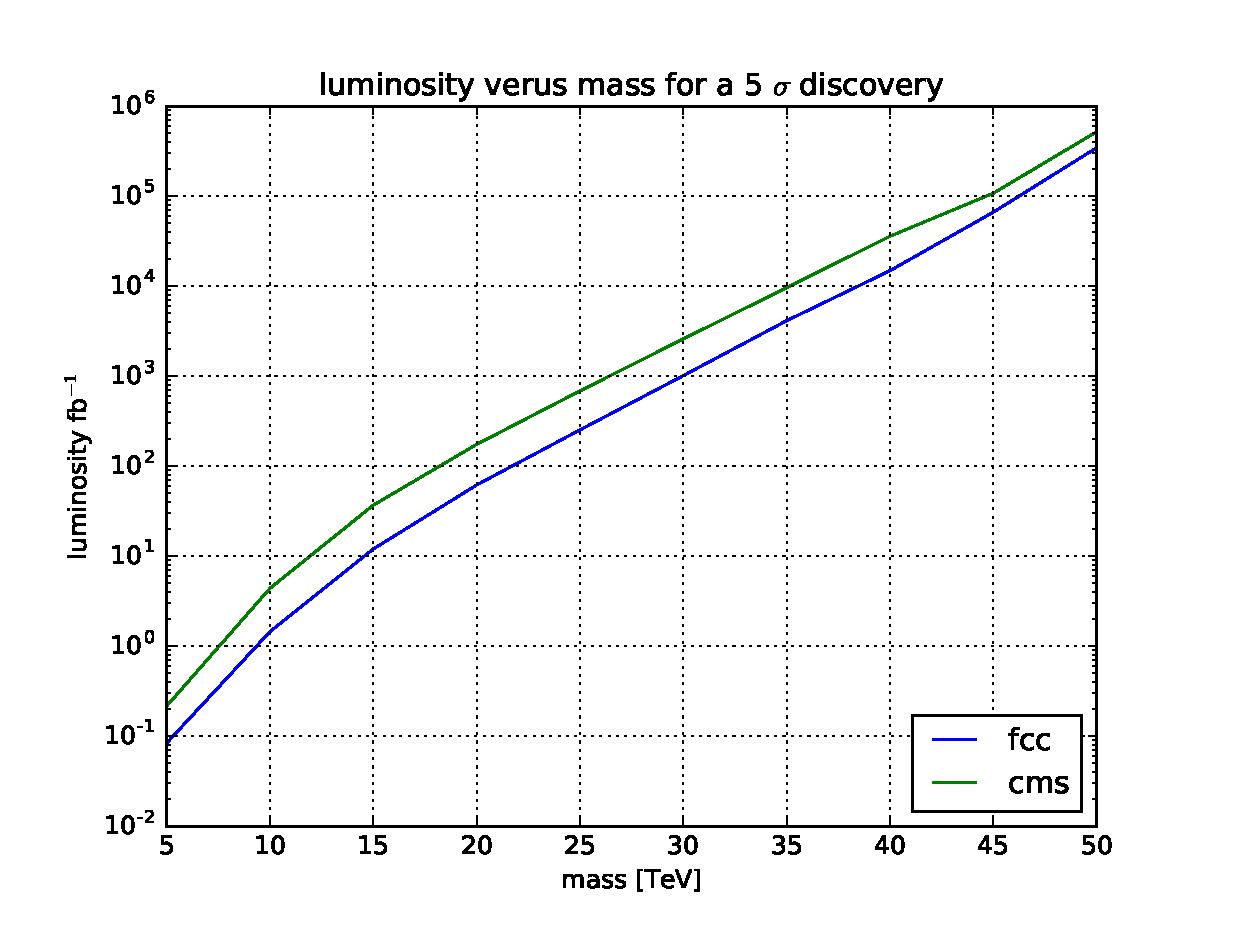
\includegraphics[width=0.495\textwidth]{Fig/DiscoveryPotential_ll.eps}
%\caption{Limit versus mass (left) and luminosity for a $5\sigma$ discovery (right) for the
% di-lepton channel combined.}
%\label{fig:zpll_lim}
%\end{figure}

\clearpage
\newpage

%%%%%%%%%%%%%%%%%%%%%%%%%%%%%%%%%%%%%%%%%%%%%%%%%%%%%
%%%%%%%%%%%%%%%%%%%%%%%%%%%%%%%%%%%%%%%%%%%%%%%%%%%%%
\subsection{Hadronic resonances : WW, $t\bar{t}$, jj}
\label{subsec:hadreso}

\subsubsection{Introduction}
Many models of beyond the SM (BSM) physics predict additional particles with masses at the TeV scale. The presence of new resonant states~\cite{Harris:2011bh,Boelaert:2009jm,Lee:1973iz,Branco:2011iw,Hill:1994hp,Kaplan:1983sm,Bellazzini:2014yua,Randall:1999ee,Pomarol:1999ad} decaying to two highly boosted particles decaying hadronically could be observed as an excess in the QCD dijet distribution. We focus here on three specific benchmark models: a \ZpSSM~\cite{Langacker:2008yv}, a Randall-Sundrum graviton~\cite{Randall:1999ee}, and an excited quark resonance~\cite{Baur:1987ga,Baur:1989kv}. We study the sensitivity in the following decay using hadronic decay modes: \zptt, \rsg\ and \qjj.

The decay products are typically in the multi-TeV regime and their reconstruction imposes stringent requirement on the detector design. Precise jet energy resolution requires full longitudinal shower containment. Highly boosted top quarks and $W$ bosons decay into highly collimated jets that need to  be disentangled from standard QCD jets by studying their substructure. High discrimination power and sensitivity for these searches at such extreme energies, requires excellent granularity both in the tracking detectors and calorimeters.

%%%%%%%%%%%%%%%%%%%%%%%%%%%%%%%%%%%%%%%%%%%%%%%%%%%%%%%%%%%%%%%%%%%%%%%%%%%%%%%%%%%%%%%%%%%%
\subsubsection{Monte Carlo Samples}
Signal models were generated with {\scshape Pythia}~8.230~\cite{Sjostrand:2014zea} and the LO cross-section is used. The SM backgrounds are di-jet (QCD), top pairs (\ttbar), $VV$ and \vj\ where $V=W/Z$, which were generated using {\scshape MG5\_}a{\scshape MC@NLO}~2.5.2~\cite{Alwall:2014} at LO. A k-factor of 2 to all the background processes.

%%%%%%%%%%%%%%%%%%%%%%%%%%%%%%%%%%%%%%%%%%%%%%%%%%%%%%%%%%%%%%%%%%%%%%%%%%%%%%%%%%%%%%%%%%%%
\subsubsection{Event Selection}

\subparagraph{Dijet analysis}

Jets are clustered using particle-flow candidates with the anti-$k_T$~\cite{Cacciari:2008gp} algorithm with parameter R=0.4. We require at least two jets with $\pt$>3~TeV and $|\eta<3|$ and the rapidity difference between the two leading jets to be small, $\Delta(\eta)<1.5$ as di-jet events will tend to be more central. The dijet invariant mass of the \qjj\ signal for $m_Q^{*}$ and QCD contributions after the full event selection is shown in Figure~\ref{figure:hadronicresonances:ttsel08} (left).

\subparagraph{Boosted Top and W analyses}

As track jets are better able to resolve the jet sub-structure compared to particle-flow jets, the jet selection for the \rsg\ and \zptt\ searches using track jets. As no lepton veto is applied, there is also some acceptance for leptonic decays. The sensitivity to semi-leptonic $WW$ or \ttbar\ decays is enhanced by adding the $\metvec$ vector to the closest jet 4-momentum (among the to leading jets).

We require two jets with a $\pt$>3~TeV and $|\eta<3|$ and $\Delta(\eta)<2.4$. Both jets must either be $W$ or top tagged (section~\cite{subsec:mvatagger}) by requiring multivariate tagger > 0.15. Both high-\pt\ jets must be $b$-tagged for the \zptt\ analysis. Finally, to further reject QCD, we require for both jets $m_{SD}>40$~GeV. In Figure~\ref{figure:hadronicresonances:ttsel08} we show the di-jet invariant mass distribution after the final cuts for the \rsg\ (center) and \zptt\ (right) analyses respectively.

\begin{figure}
  \centering
  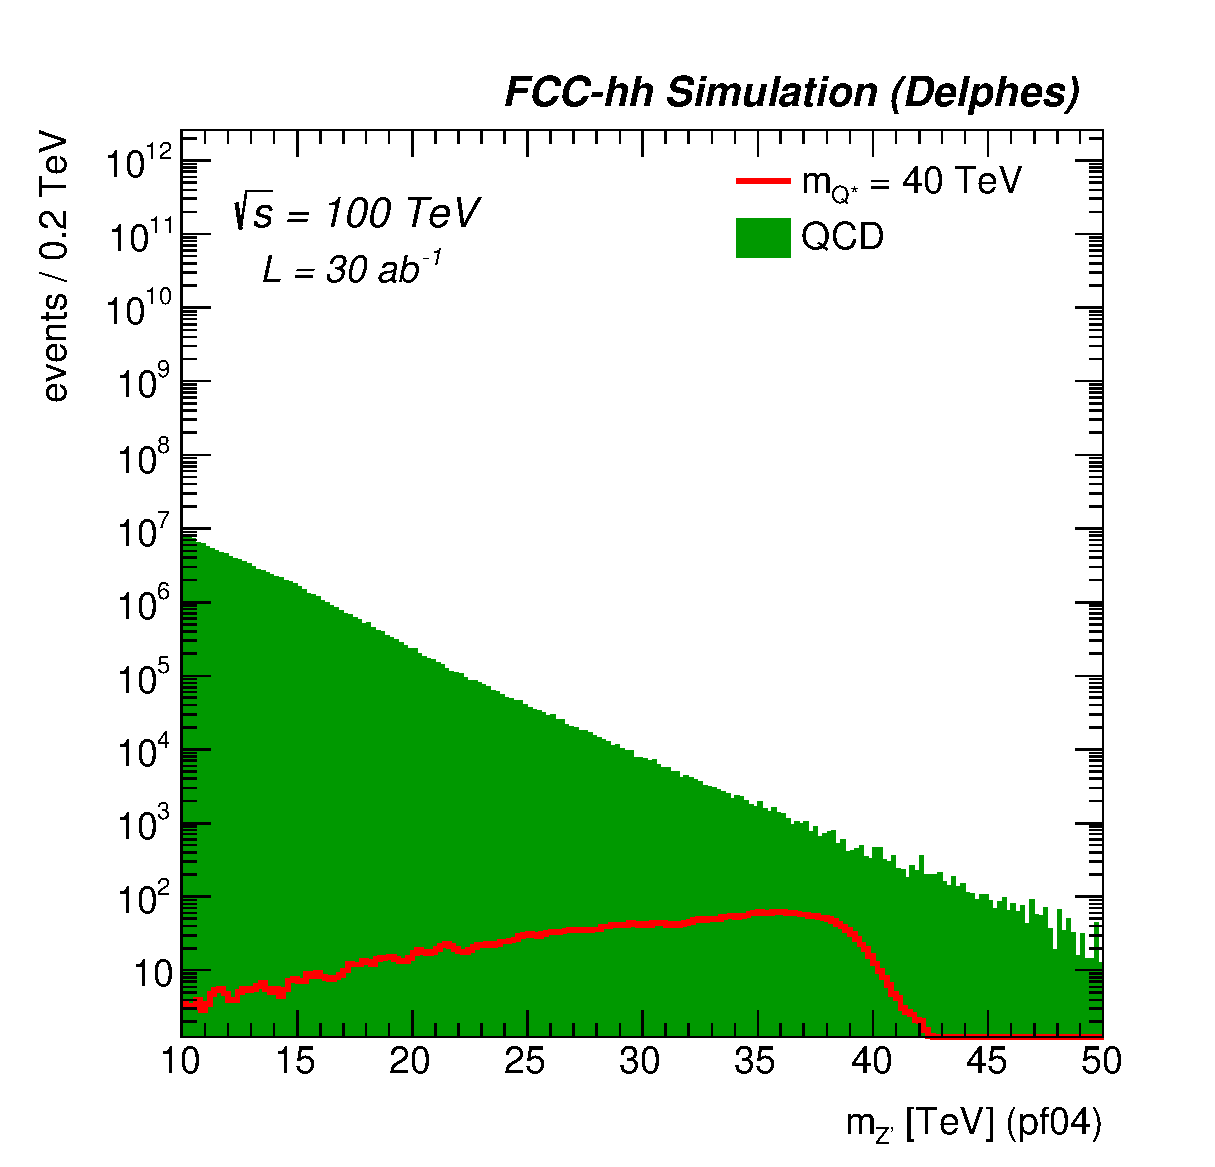
\includegraphics[width=0.30\columnwidth]{Fig/Mj1j2_pf04_sel1_nostack_log.eps}
  \includegraphics[width=0.30\columnwidth]{Fig/Mj1j2_pf08_fit_sel4_nostack_log.eps}
  \includegraphics[width=0.30\columnwidth]{Fig/Mj1j2_pf08_MetCorr_fit_sel8_nostack_log.eps}
  \caption{Invariant mass distribution of the two leading jets for the pre-selection (left) and full selection (right) for a 20~TeV signal for the \qjj\ (left), \zptt\ (center) and \rsg\ (right) analyses.\MS{need editing / style}}
  \label{figure:hadronicresonances:ttsel08}
\end{figure}

\begin{table}[htbp]
   \centering
\begin{tabular}{|c|c|c|c|c|c|c|c|c|}
  \hline
  & \multicolumn{2}{c|}{di-jet}  & \multicolumn{2}{c|}{$\ttbar$} & \multicolumn{2}{c|}{WW} \\
  \cline{2-7}

 & pre-sel & final-sel  & pre-sel & final-sel & pre-sel & final-sel\\
  \hline
  di-jet & 385555434 &  373661126 &  154855591 & 11439.8&  154856148 & 64484\\
  $\ttbar$ & - & - & 1114779 & 74193.6 &  1114779 & 3185\\
  di-bosons & - & - &  41820 &  17.1 &  41820 & 6092\\
  boson+jet & - & - & 1610472 & 264.1&  1610472 & 25377\\
  \hline
  total bkg  &  385555434& 373661126& 157622662 & 85914 & 154856148 & 99137\\
  \hline
  10~TeV &  - & - &  101529 & 15601 &  47853 & 15745\\
  20~TeV &   1253072 &  1239813& 7774 & 500.6 & 1282 & 578\\
  30~TeV &  69922 &  67488 & 485.2 & 13.2 &  61.4 & 30.1 \\
  40~TeV &  4589 &  4373 & - & - & - & -\\
  \hline
\end{tabular}
  \caption{Yields for the di-jet, $\ttbar$ and WW analyses after pre and final selection.}
  \label{tab:hadronicresonances:yields}
\end{table}

%%%%%%%%%%%%%%%%%%%%%%%%%%%%%%%%%%%%%%%%%%%%%%%%%%%%%%%%%%%%%%%%%%%%%%%%%%%%%%%%%%%%%%%%%%%%
\subsubsection{Signal extraction and results}
Hypothesis testing is performed using a modified frequentist method based on a profile likelihood fit that takes into account the systematic uncertainties as nuisance parameters. The di-jet invariant mass is used as a discriminant. In order to reduce large statistical fluctuations from high Monte Carlo weight events, we parameterize the background invariant mass distribution with the following function (conservatively assuming 50\% uncertainty on the background normalisation) $f(z)=p_1(1-z)^{p_2}z^{p_3}z^{p_{4}logz}$, where $z=m_{jj}/\sqrt{s}$.

The expected exclusion limits at 95\% CL are shown in Figures~\ref{figure:hadronicresonances:limits} and~\ref{figure:hadronicresonances:resultsjj}. For the \qjj\ masses up to 40~TeV could be discovered with \intlumifcc. Reconstructing Heavy resonances decaying to $WW$ and \ttbar\ is more challenging and requires the use of novel approaches to boosted object tagging to reduce the backgrounds. The reach for \zptt\ (in TC2 models) and \rsg\ is 24~TeV and 22~TeV respectively and it is possible to discover a $Z^{\prime}_{SSM} \rightarrow \ttbar$ up to $m_{Z}=18$~TeV.

\begin{figure}
  \centering
  \includegraphics[width=0.30\columnwidth]{Fig/lim_Qstar_jj_fcc_v02.eps}
  \includegraphics[width=0.30\columnwidth]{Fig/lim_RSGraviton_ww_fcc_v02.eps}
  \includegraphics[width=0.30\columnwidth]{Fig/lim_Zprime_tt_fcc_v02.eps}
  \caption{Exclusion limit at 95\% CL versus heavy resonance mass decaying into di-jet (left), WW (center), \ttbar\ (right).}
  \label{figure:hadronicresonances:limits}
\end{figure}

\begin{figure}
  \centering
  \includegraphics[width=0.30\columnwidth]{Fig/DiscoveryPotential_jj_rootStyle.eps}
  \includegraphics[width=0.30\columnwidth]{Fig/DiscoveryPotential_ww_tagger_rootStyle.eps}
  \includegraphics[width=0.30\columnwidth]{Fig/DiscoveryPotential_tt_SSM_TC2_tagger_TRFbtag_rootStyle.eps}
  \caption{Integrated luminosity for a $5\sigma$ discovery as a function of the heavy resonance mass decaying into di-jet (left), WW (center), \ttbar\ (right).}
  \label{figure:hadronicresonances:resultsjj}
\end{figure}

%%%%%%%%%%%%%%%%%%%%%%%%%%%%%%%%%%%%%%%%%%%%%%%%%%%%%
% material :

% ttbar
% Backgrounds: QCD, ttbar, single top, V+jets, VV. 

\begin{landscape}
\begin{table}[!htb]\centering
\scalebox{0.9}{
\begin{tabular}{|c|c|c|c|c|c|c|}
\hline
\hline
\multicolumn{2}{|c|}{}          & preselection                                                & cut1                                    & cut2                                    & tagger1                         & tagger2                                \\
\hline
\multicolumn{2}{|c|}{selection} & $Jet_{1,2}^{trk02 SD Corr}~\pT$ > 3 TeV                     & preselection +                          & cut1 +                                  & preselection +                  & tagger1 +                              \\
\multicolumn{2}{|c|}{}          & |$Jet_{1,2}^{trk02 SD Corr}~\eta$| < 3                      & 0.3 < $Jet_{1}^{trk02}~\tau_{21}$ < 0.7 & 0.3 < $Jet_{2}^{trk02}~\tau_{21}$ < 0.7 & $Jet_{1,2}~t/QCD tagger$ > 0.15 & $Jet_{1,2}^{trk02 SD Corr}~M$ > 40 GeV \\
\multicolumn{2}{|c|}{}          & $Jet_{1,2}^{trk02}~\tau_{21,31,32}$ > 0                     & $Jet_{1}^{trk02}~\tau_{32}$ < 0.7       & $Jet_{2}^{trk02}~\tau_{32}$ < 0.75      &                                 &                                        \\
\multicolumn{2}{|c|}{}          & |$\Delta(Jet_{1}^{trk02}~\eta,Jet_{2}^{trk02}~\eta]$| < 2.4 & $Jet_{1}^{trk02 SD Corr}~M$ > 100 GeV   & $Jet_{2}^{trk02 SD Corr}~M$ > 100 GeV   &                                 &                                        \\
\multicolumn{2}{|c|}{}          & $M_{Jet_{1},Jet_{2}}^{METcorr}$(pf08) > 5 GeV   &    &   &   &  \\
\hline
\hline
background      & vv            & 41820.4 (4680415)     & 1470.3 (54701)       & 32.9 (2639)        & 7108.8 (699592)    & 6998.2 (684387)    \\
                & vj            & 1610471.9 (5952097)   & 70863.5 (416614)     & 2390.4 (20401)     & 107224.0 (193932)  & 103957.7 (184953)  \\
                & tt            & 1114779.3 (7919918)   & 472480.2 (3591669)   & 209659.6 (1719905) & 257401.2 (2008578) & 253906.9 (1962131) \\
                & QCD           & 154855591.0 (7255490) & 16915580.5 (1041418) & 2846240.2 (185371) & 2848680.2 (49597)  & 2777145.0 (46160)  \\
                & Total         & 157622662.489         & 17460394.591         & 3058323.073        & 3220414.127        & 3142007.794        \\
\hline
signal $m_{Z}$= & 10 TeV        & 101529.3 (152148)     & 48915.6 (73303)      & 27591.1 (41347)    & 49198.5 (73727)    & 48415.1 (72553)    \\
                & 15 TeV        & 31764.0 (338548)      & 14769.1 (157413)     & 7459.6 (79506)     & 13254.8 (141273)   & 12943.0 (137949)   \\
                & 20 TeV        & 7774.6 (454632)       & 3560.7 (208219)      & 1702.5 (99554)     & 2594.2 (151698)    & 2530.2 (147958)    \\
                & 25 TeV        & 1925.9 (457629)       & 866.8 (205952)       & 402.0 (95509)      & 491.4 (116768)     & 479.8 (114007)     \\
                & 30 TeV        & 485.2 (444228)        & 216.1 (197850)       & 98.3 (90011)       & 97.1 (88884)       & 94.8 (86815)       \\
                & 35 TeV        & 123.9 (367937)        & 54.3 (161321)        & 24.6 (72905)       & 21.2 (62926)       & 20.7 (61419)       \\
\hline
\hline
\end{tabular}}
\caption{Summary of $\Zp \rightarrow \ttbar$ analysis cut-flow.}
\label{tab:Zptt_cutflow}
\end{table}
\end{landscape}

\begin{landscape}
\begin{table}[!htb]\centering
\begin{tabular}{|c|c|c|c|c|c|}
\hline
\hline
\multicolumn{2}{|c|}{}          & btag1 & btag2                      & btag3 & btag4                   \\
\hline
\multicolumn{2}{|c|}{selection} & cut2 + & tagger2 +                 & cut2 + & tagger2 +              \\
\multicolumn{2}{|c|}{}          & \multicolumn{2}{c|}{2 direct btag} & \multicolumn{2}{c|}{2 TRF btag} \\
\multicolumn{2}{|c|}{}          & \multicolumn{4}{c|}{(on the 2 leading jets)}                         \\
\multicolumn{2}{|c|}{}          & \multicolumn{4}{c|}{}                                                \\
\hline
\hline
background      & vv            & 0.0 (3)          & 20.4 (2115)      & 0.5 (2639)        & 17.1 (684387)     \\
                & vj            & 13.3 (69)        & 394.2 (650)      & 5.4 (20401)       & 264.1 (184953)    \\
                & tt            & 50372.8 (271482) & 87680.8 (498579) & 54627.4 (1719905) & 74193.6 (1962131) \\
                & QCD           & 27551.7 (576)    & 23051.2 (331)    & 10999.0 (185371)  & 11439.8 (46160)   \\
                & Total         & 77937.847        & 111146.632       & 65632.28          & 85914.564         \\
\hline
signal $m_{Z}$= & 10 TeV        & 10247.8 (15357)  & 18311.6 (27441)  & 9278.1 (41347)    & 15601.6 (72553)   \\
                & 15 TeV        & 2133.7 (22742)   & 3850.8 (41043)   & 1876.4 (79506)    & 3305.5 (137949)   \\
                & 20 TeV        & 350.1 (20471)    & 584.7 (34190)    & 303.7 (99554)     & 500.6 (147958)    \\
                & 25 TeV        & 59.0 (14019)     & 87.7 (20845)     & 50.4 (95509)      & 75.9 (114007)     \\
                & 30 TeV        & 10.7 (9809)      & 15.5 (14185)     & 9.1 (90011)       & 13.2 (86815)      \\
                & 35 TeV        & 2.4 (7039)       & 3.6 (10681)      & 2.0 (72905)       & 3.1 (61419)       \\
\hline
\hline
\end{tabular}
\caption{Summary of $\Zp \rightarrow \ttbar$ analysis cut-flow at b-tagging level.}
\label{tab:Zptt_cutflow_btag}
\end{table}
\end{landscape}

\begin{figure}[!htb]\centering
\includegraphics[width=0.8\textwidth]{Fig/Zptt/rapiditySeparation_sel0_before_cut_nostack_log.eps}
\caption{Rapidity separation at preselection level before cut on this variable in $\Zp \rightarrow \ttbar$ analysis. The generated mass of the signal sample is 10 $\TeV$.}
\label{fig:Zptt_sel0_rapidity}
\end{figure}

\begin{figure}[!htb]\centering
\includegraphics[width=0.495\textwidth]{Fig/Zptt/Jet1_trk02_SD_Cor_m_sel0_nostack_log.eps}
\includegraphics[width=0.495\textwidth]{Fig/Zptt/Jet1_tau21_sel0_nostack_log.eps}
\includegraphics[width=0.495\textwidth]{Fig/Zptt/Jet1_tau32_sel0_nostack_log.eps}
\caption{Variables used for the first step of cuts in cut-based analysis at preselection level for leading jet $\pT$ in $\Zp \rightarrow \ttbar$ analysis : jet mass SD (Soft-Dropped) corrected, jet $\tau_{21}$ and jet $\tau_{32}$. The generated mass of the signal sample is 10 $\TeV$.}
\label{fig:Zptt_sel0_cut}
\end{figure}

\begin{figure}[!htb]\centering
\includegraphics[width=0.495\textwidth]{Fig/Zptt/Jet2_trk02_SD_Cor_m_sel1_nostack_log.eps}
\includegraphics[width=0.495\textwidth]{Fig/Zptt/Jet2_tau21_sel1_nostack_log.eps}
\includegraphics[width=0.495\textwidth]{Fig/Zptt/Jet2_tau32_sel1_nostack_log.eps}
\caption{Variables used for the second step of cuts in cut-based analysis after first set of cuts for second leading jet $\pT$ in $\Zp \rightarrow \ttbar$ analysis : jet mass SD (Soft-Dropped) corrected, jet $\tau_{21}$ and jet $\tau_{32}$. The generated mass of the signal sample is 10 $\TeV$.}
\label{fig:Zptt_sel1_cut}
\end{figure}

\begin{figure}[!htb]\centering
\includegraphics[width=0.495\textwidth]{Fig/Zptt/Jet1_thad_vs_QCD_tagger_sel0_nostack_log.eps}
\includegraphics[width=0.495\textwidth]{Fig/Zptt/Jet2_thad_vs_QCD_tagger_sel0_nostack_log.eps}
\caption{top Vs QCD tagger at preselection level for leading jet (left) and second leading jet $\pT$ (right) in $\Zp \rightarrow \ttbar$ analysis. The generated mass of the signal sample is 10 $\TeV$.}
\label{fig:Zptt_sel0_tagger}
\end{figure}

\begin{figure}[!htb]\centering
\includegraphics[width=0.495\textwidth]{Fig/Zptt/Jet1_trk02_SD_Cor_m_sel3_nostack_log.eps}
\includegraphics[width=0.495\textwidth]{Fig/Zptt/Jet2_trk02_SD_Cor_m_sel3_nostack_log.eps}
\caption{Jet mass SD (Soft-Dropped) corrected in anti-QCD tagger-based analysis after first set of cuts for leading jet (left) and second leading jet $\pT$ (right) in $\Zp \rightarrow \ttbar$ analysis. The generated mass of the signal sample is 10 $\TeV$.}
\label{fig:RSGww_sel1_tagger}
\end{figure}

% no eps
\begin{figure}[!htb]\centering
\includegraphics[width=0.495\textwidth]{Fig/check_TRF/Zptt/jet12pdgID_QCD5f_redModule_blueDELPHES.png}
\includegraphics[width=0.495\textwidth]{Fig/check_TRF/Zptt/jet12pdgID_ttbar_redModule_blueDELPHES.png}
\includegraphics[width=0.495\textwidth]{Fig/check_TRF/Zptt/jet12pdgID_Zptt10TeV_redModule_blueDELPHES.png}
\includegraphics[width=0.495\textwidth]{Fig/check_TRF/Zptt/TRF2tagex_module_redZptt10TeV_blackQCD_bluettbar.png}
\caption{Checks of pdgID obtained from recomputation (red) compared to Delphes information (blue) for leading jet (continuous line) and second leading jet $\pT$ (dashed line), and for QCD (top left), $\ttbar$ (top right) and $\Zp \rightarrow \ttbar$ 10 $\TeV$ (bottom left) samples in $\Zp \rightarrow \ttbar$ analysis. Tag Rate Function for a two b-tagged jets event computed from the two leading jets only of the event (bottom right) for QCD (black), $\ttbar$ blue) and $\Zp \rightarrow \ttbar$ 10 $\TeV$ (red) samples.}
\label{fig:Zptt_TRFchecks}
\end{figure}

% no eps
\begin{figure}[!htb]\centering
\includegraphics[width=0.495\textwidth]{Fig/check_TRF/tth_boosted/jet12pdgID_ttbb_redModule_blueDELPHES.png}
\includegraphics[width=0.495\textwidth]{Fig/check_TRF/tth_boosted/jet12pdgID_ttj_redModule_blueDELPHES.png}
\includegraphics[width=0.495\textwidth]{Fig/check_TRF/tth_boosted/jet12pdgID_ttz_redModule_blueDELPHES.png}
\includegraphics[width=0.495\textwidth]{Fig/check_TRF/tth_boosted/jet12pdgID_tth_redModule_blueDELPHES.png}
\caption{Checks of pdgID obtained from recomputation (red) compared to Delphes information (blue) for leading jet (continuous line) and second leading jet $\pT$ (dashed line), and for $\ttbb$ (top left), $\ttj$ (top right), $\ttz$ (bottom left) and $\tthbb$ (bottom right) samples in $\tthbb$ boosted analysis.}
\label{fig:tthboosted_TRFchecks1}
\end{figure}

% no eps
\begin{figure}[!htb]\centering
\includegraphics[width=0.495\textwidth]{Fig/check_TRF/tth_boosted/jet34pdgID_ttbb_redModule_blueDELPHES.png}
\includegraphics[width=0.495\textwidth]{Fig/check_TRF/tth_boosted/jet34pdgID_ttj_redModule_blueDELPHES.png}
\includegraphics[width=0.495\textwidth]{Fig/check_TRF/tth_boosted/jet34pdgID_ttz_redModule_blueDELPHES.png}
\includegraphics[width=0.495\textwidth]{Fig/check_TRF/tth_boosted/jet34pdgID_tth_redModule_blueDELPHES.png}
\caption{Checks of pdgID obtained from recomputation (red) compared to Delphes information (blue) for third leading jet (continuous line) and fourth leading jet $\pT$ (dashed line), and for $\ttbb$ (top left), $\ttj$ (top right), $\ttz$ (bottom left) and $\tthbb$ (bottom right) samples in $\tthbb$ boosted analysis.}
\label{fig:tthboosted_TRFchecks2}
\end{figure}

\begin{figure}[!htb]\centering
\includegraphics[width=0.495\textwidth]{Fig/Zptt/Mj1j2_pf08_MetCorr_fit_sel2_nostack_log.eps}
\includegraphics[width=0.495\textwidth]{Fig/Zptt/Mj1j2_pf08_MetCorr_fit_sel4_nostack_log.eps}
\includegraphics[width=0.495\textwidth]{Fig/Zptt/Mj1j2_pf08_MetCorr_fit_sel5_nostack_log.eps}
\includegraphics[width=0.495\textwidth]{Fig/Zptt/Mj1j2_pf08_MetCorr_fit_sel6_nostack_log.eps}
\includegraphics[width=0.495\textwidth]{Fig/Zptt/Mj1j2_pf08_MetCorr_fit_sel7_nostack_log.eps}
\includegraphics[width=0.495\textwidth]{Fig/Zptt/Mj1j2_pf08_MetCorr_fit_sel8_nostack_log.eps}
\caption{Zprime mass after the full selection for anaylsis cut-based (left) and anti-QCD tagger based (right), and for the b-tagging scenarios : before b-tag (top), direct 2 b-tag (middle) and Tag Rate Function 2 b-tag (bottom) in $\Zp \rightarrow \ttbar$ analysis. The generated mass of the signal sample is 10 $\TeV$.}
\label{fig:Zptt_mass_sel_final}
\end{figure}

\begin{figure}[!htb]\centering
\includegraphics[width=0.495\textwidth]{Fig/Zptt/lim_Zprime_tt_fcc_v02_cut.eps}
\includegraphics[width=0.495\textwidth]{Fig/Zptt/DiscoveryPotential_tt_cut_rootStyle.eps}
\includegraphics[width=0.495\textwidth]{Fig/Zptt/lim_Zprime_tt_fcc_v02_tagger.eps}
\includegraphics[width=0.495\textwidth]{Fig/Zptt/DiscoveryPotential_tt_TC2_tagger_rootStyle.eps}
\caption{Limit (left) and discovery potential (right) for analysis cut-based with direct b-tagging (top) and anti-QCD tagger-based with direct b-tagging (bottom) in $\Zp \rightarrow \ttbar$ analysis. Default model used for discovery potential is TC2.}
\label{fig:Zptt_limit_direct}
\end{figure}

\begin{figure}[!htb]\centering
\includegraphics[width=0.495\textwidth]{Fig/Zptt/lim_Zprime_tt_fcc_v02_cut_TRFbtag.eps}
\includegraphics[width=0.495\textwidth]{Fig/Zptt/DiscoveryPotential_tt_cut_TRFbtag_rootStyle.eps}
\includegraphics[width=0.495\textwidth]{Fig/Zptt/lim_Zprime_tt_fcc_v02_tagger_TRFbtag.eps}
\includegraphics[width=0.495\textwidth]{Fig/Zptt/DiscoveryPotential_tt_SSM_TC2_tagger_TRFbtag_rootStyle.eps}
\caption{Limit (left) and discovery potential (right) for analysis cut-based with TRF b-tagging (top) and anti-QCD tagger-based with TRF b-tagging (bottom) in $\Zp \rightarrow \ttbar$ analysis. Default model used for discovery potential is TC2 in the top plot. The bottom discovery plot shows the comparison between the TC2 default model (red line) and the SSM one (blue line).}
\label{fig:Zptt_limit_trf}
\end{figure}

\clearpage
\newpage

% WW
% Backgrounds: QCD multijet, V+jets, VV.

\begin{landscape}
\begin{table}[!htb]\centering
\scalebox{0.9}{
\begin{tabular}{|c|c|c|c|c|c|c|}
\hline
\hline
\multicolumn{2}{|c|}{}          & preselection                                                & cut1                                         & cut2                                    & tagger1                         & tagger2                                \\
\hline
\multicolumn{2}{|c|}{selection} & $Jet_{1,2}^{trk02 SD Corr}~\pT$ > 3 TeV                     & preselection +                               & cut1 +                                  & preselection +                  & tagger1 +                              \\
\multicolumn{2}{|c|}{}          & |$Jet_{1,2}^{trk02 SD Corr}~\eta$| < 3                      & 0.3 < $Jet_{1,2}^{trk02}~\tau_{21}$ < 0.6    & $Jet_{1,2}~Flow_{45}$ < 0.07 & $Jet_{1,2}~W/QCD tagger$ > 0.15 & $Jet_{1,2}^{trk02 SD Corr}~M$ > 40 GeV \\
\multicolumn{2}{|c|}{}          & $Jet_{1,2}^{trk02}~\tau_{21,31,32}$ > 0                     & 50 > $Jet_{1,2}^{trk02 SD Corr}~M$ > 100 GeV & $Jet_{1,2}~Flow_{55}$ < 0.07 &                                 &                                        \\
\multicolumn{2}{|c|}{}          & |$\Delta(Jet_{1}^{trk02}~\eta,Jet_{2}^{trk02}~\eta]$| < 2.4 &                                              &                              &                                 &                                        \\
\multicolumn{2}{|c|}{}          & $M_{Jet_{1},Jet_{2}}$(pf08) > 5 GeV &                                              &                              &                                 &                                        \\
\hline
\hline
background      & vv            & 41820.4 (4680415)     & 10279.3 (1915274) & 2951.8 (1383948) & 7176.3 (2732541) & 6092.4 (2217631) \\
                & vj            & 1610471.9 (5952097)   & 104360.1 (265110) & 26509.0 (161120) & 50484.8 (343202) & 25376.8 (179954) \\
                & tt            & 1114779.3 (7919918)   & 16446.1 (179682)  & 1986.7 (79261)   & 3627.4 (134680)  & 3184.8 (110218)  \\
                & QCD           & 154856148.5 (7255491) & 1621365.1 (33102) & 386147.5 (17595) & 225206.9 (14209) & 64483.7 (6051)   \\
                & Total         & 157623220.015         & 1752450.61        & 417595.057       & 286495.406       & 99137.679        \\
\hline
signal $m_{G}$= & 10 TeV        & 47853.2 (170178)      & 20640.8 (73404)   & 7035.8 (25021)   & 18168.9 (64613)  & 15745.2 (55994) \\
                & 15 TeV        & 7242.3 (264747)       & 2853.8 (104323)   & 1947.3 (71183)   & 3744.4 (136881)  & 2911.5 (106433) \\
                & 20 TeV        & 1282.5 (289346)       & 492.2 (111045)    & 412.3 (93008)    & 759.3 (171294)   & 577.8 (130354)  \\
                & 25 TeV        & 259.3 (329187)        & 97.3 (123557)     & 86.7 (110145)    & 159.3 (202235)   & 122.9 (156034)  \\
                & 30 TeV        & 61.4 (343104)         & 22.7 (126833)     & 20.7 (115782)    & 38.2 (213073)    & 30.1 (168358)   \\
                & 35 TeV        & 14.5 (314975)         & 5.2 (113783)      & 4.9 (105173)     & 9.0 (195097)     & 7.3 (157530)    \\
\hline
\hline
\end{tabular}}
\caption{Summary of $G \rightarrow WW$ analysis cut-flow.}
\label{tab:RSGww_cutflow}
\end{table}
\end{landscape}

\begin{figure}[!htb]\centering
\includegraphics[width=0.8\textwidth]{Fig/RSGww/rapiditySeparation_sel0_before_cut_nostack_log.eps}
\caption{Rapidity separation at preselection level before cut on this variable in $G \rightarrow WW$ analysis. The generated mass of the signal sample is 10 $\TeV$.}
\label{fig:RSGww_sel0_rapidity}
\end{figure}

\begin{figure}[!htb]\centering
\includegraphics[width=0.495\textwidth]{Fig/RSGww/Jet1_trk02_SD_Cor_m_sel0_nostack_log.eps}
\includegraphics[width=0.495\textwidth]{Fig/RSGww/Jet2_trk02_SD_Cor_m_sel0_nostack_log.eps}
\includegraphics[width=0.495\textwidth]{Fig/RSGww/Jet1_tau21_sel0_nostack_log.eps}
\includegraphics[width=0.495\textwidth]{Fig/RSGww/Jet2_tau21_sel0_nostack_log.eps}
\caption{Variables used for the first step of cuts in cut-based analysis at preselection level for leading jet (left) and second leading jet $\pT$ (right) in $G \rightarrow WW$ analysis : jet mass SD (Soft-Dropped) corrected (top) and jet $\tau_{21}$ (bottom). The generated mass of the signal sample is 10 $\TeV$.}
\label{fig:RSGww_sel0_cut}
\end{figure}

\begin{figure}[!htb]\centering
\includegraphics[width=0.495\textwidth]{Fig/RSGww/Jet1_Flow45_sel1_nostack_log.eps}
\includegraphics[width=0.495\textwidth]{Fig/RSGww/Jet2_Flow45_sel1_nostack_log.eps}
\includegraphics[width=0.495\textwidth]{Fig/RSGww/Jet1_Flow55_sel1_nostack_log.eps}
\includegraphics[width=0.495\textwidth]{Fig/RSGww/Jet2_Flow55_sel1_nostack_log.eps}
\caption{Variables used for the second step of cuts in cut-based analysis after first set of cuts for leading jet (left) and second leading jet $\pT$ (right) in $G \rightarrow WW$ analysis : jet Flow45 (top) and Flow55 (bottom). The generated mass of the signal sample is 10 $\TeV$.}
\label{fig:RSGww_sel1_cut}
\end{figure}

\begin{figure}[!htb]\centering
\includegraphics[width=0.495\textwidth]{Fig/RSGww/Jet1_Whad_vs_QCD_tagger_sel0_nostack_log.eps}
\includegraphics[width=0.495\textwidth]{Fig/RSGww/Jet2_Whad_vs_QCD_tagger_sel0_nostack_log.eps}
\caption{W Vs QCD tagger at preselection level for leading jet (left) and second leading jet $\pT$ (right) in $G \rightarrow WW$ analysis. The generated mass of the signal sample is 10 $\TeV$.}
\label{fig:RSGww_sel0_tagger}
\end{figure}

\begin{figure}[!htb]\centering
\includegraphics[width=0.495\textwidth]{Fig/RSGww/Jet1_trk02_SD_Cor_m_sel3_nostack_log.eps}
\includegraphics[width=0.495\textwidth]{Fig/RSGww/Jet2_trk02_SD_Cor_m_sel3_nostack_log.eps}
\caption{Jet mass SD (Soft-Dropped) corrected in anti-QCD tagger-based analysis after first set of cuts for leading jet (left) and second leading jet $\pT$ (right) in $G \rightarrow WW$ analysis. The generated mass of the signal sample is 10 $\TeV$.}
\label{fig:RSGww_sel1_tagger}
\end{figure}

\begin{figure}[!htb]\centering
\includegraphics[width=0.495\textwidth]{Fig/RSGww/Mj1j2_pf08_fit_sel2_nostack_log.eps}
\includegraphics[width=0.495\textwidth]{Fig/RSGww/Mj1j2_pf08_fit_sel4_nostack_log.eps}
\caption{RSG mass after the full selection for analysis cut-based (left) and anti-QCD tagger-based (right). The generated mass of the signal sample is 10 $\TeV$.}
\label{fig:RSGww_mass_sel_final}
\end{figure}

\begin{figure}[!htb]\centering
\includegraphics[width=0.495\textwidth]{Fig/RSGww/lim_RSGraviton_ww_fcc_v02_cut.eps}
\includegraphics[width=0.495\textwidth]{Fig/RSGww/DiscoveryPotential_ww_cut_rootStyle.eps}
\includegraphics[width=0.495\textwidth]{Fig/RSGww/lim_RSGraviton_ww_fcc_v02_tagger.eps}
\includegraphics[width=0.495\textwidth]{Fig/RSGww/DiscoveryPotential_ww_tagger_rootStyle.eps}
\caption{Limit (left) and discovery potential (right) for analysis cut-based (top) and anti-QCD tagger-based (bottom) in $G \rightarrow WW$ analysis.}
\label{fig:RSWww_limit}
\end{figure}

\clearpage
\newpage


%%%%%%%%%%%%%%%%%%%%%%%%%%%%%%%%%%%%%%%%%%%%%%%%%%%%%
%%%%%%%%%%%%%%%%%%%%%%%%%%%%%%%%%%%%%%%%%%%%%%%%%%%%%
\section{Comparison with $27 TeV HE-HLC$}
\label{sec:ana27tev}
- explain diff of the analysis with 100 TeV and show final plots as in Yellow report.
- add section for different models study

%%%%%%%%%%%%%%%%%%%%%%%%%%%%%%%%%%%%%%%%%%%%%%%%%%%%%
%%%%%%%%%%%%%%%%%%%%%%%%%%%%%%%%%%%%%%%%%%%%%%%%%%%%%
\section{Conclusion}
This note presents preliminary studies of a search for $\Zp$ 
bosons decaying into two electrons or muons in the FCC context. The expected number 
of signal and background events have been estimated from simulated truth level information 
after applying smearing functions to mimic the FCC detector response.
Using a cut-based analysis and assuming simplistic systematic uncertainties, $\ZpSSM$
masses below 40 $\TeV$ can be excluded at 95$\%$ C.L. 
using 30 $\afb{}$ of data. 

\bibliographystyle{plain}
\bibliography{bibliography.bib}
\end{document}
